\chapter{Parameter Estimation} \label{cha:parameterEstimation}
A central part in modelling is parameter estimation and its importance is often underestimated. If the parameters in the model are not well estimated several problems arise when trying to synthesise model-based controllers. If a system's dynamics are completely unknown a black box method is used \emph{i.e.} general equations are fitted to test data. When a system can be completely modelled analytically for example via Newtons laws it is called white box modelling. In this thesis the model structure of the system is known but several physical parameters are unknown, this is called gray box modelling. 

To estimate the unknown parameters in the \abbrROV model described in \Chapterref{cha:modelling} different methods can be used. Relations between states can be used to get better estimates of parameters for example if the angles of the \abbrROV are estimated well the relations
\begin{align}
\rolldot &= p + q \sin \rollAngle \tan \pitchAngle + r \cos \rollAngle \tan \pitchAngle,\\
\pitchdot &= q \cos \rollAngle - r \sin \rollAngle \\
&\textrm{and} \nonumber \\
\yawdot &= q \frac{\sin \rollAngle}{\cos \pitchAngle} + r \frac{\cos \rollAngle}{\cos \pitchAngle}
\end{align}
from \Chapterref{cha:modelling} could be used. Another aspect to consider when estimating model parameters is what to use as inputs and what to use as outputs. Inputs to a system are considered to be true signals, thus if they are noisy or inaccurate they can effect the estimation negatively. Outputs from a system are measurements of a state, thus they are considered to be somewhat uncertain. To make estimation more convenient the attitude model structure from \Chapterref{cha:modelling} is reduced to 
\begin{multline} \label{eq:p_dotWithoutTranslation}
\pdot = \frac{\thrusterfun{1} \distance{y}{1} - \thrusterfun{2} \distance{y}{2} + \thrusterfun{6} \distance{z}{6}}{\Ix - \Kpdot} + \frac{p (\Kp + \Kpabsp \abs{p})}{\Ix - \Kpdot} + \frac{-\Mqdot q r}{\Ix - \Kpdot} + \frac{\Nrdot q r}{\Ix - \Kpdot} +\\
\frac{q r (\Iy - \Iz)}{\Ix - \Kpdot} + \frac{B \cos{\theta} \sin{\phi} z_B}{\Ix - \Kpdot},
\end{multline} 
\begin{multline} \label{eq:q_dotWithoutTranslation}
\qdot =\frac{\thrusterfun{1} \distance{x}{1} + \thrusterfun{2} \distance{x}{2} - \thrusterfun{5} \distance{x}{5}}{\Iy - \Mqdot} + \frac{q (\Mq + \Mqabsq \abs{q})}{\Iy - \Mqdot} + \frac{\Kpdot p r}{\Iy - \Mqdot} + \frac{-\Nrdot p r}{\Iy - \Mqdot} +\\
\frac{p r (\Iz - \Ix)}{\Iy - \Mqdot} + \frac{B \sin{\theta} z_B}{\Iy - \Mqdot}\ \textrm{and}
\end{multline} 
\begin{multline} \label{eq:r_dotWithoutTranslation}
\rdot = \frac{\thrusterfun{3} \distance{y}{3} - \thrusterfun{4} \distance{y}{4}}{\Iz - \Nrdot} + \frac{r (\Nr + \Nrabsr \abs{r})}{\Iz - \Nrdot} + \frac{-\Kpdot p q}{\Iz - \Nrdot} + \frac{\Mqdot p q}{\Iz - \Nrdot} + \frac{p q (\Ix - \Iy)}{\Iz - \Nrdot}
\end{multline} 
This can be done because the translation dynamics in the attitude model structure are assumed to be small during tests. The \abbrROV has neutral buoyancy thus $B = W$ in this Chapter.

%%%%%%%%%%%%%%%%%%%%%%%%%%%%%%%%%%%%%%%%%%%%%%%%%%%%%%%%%%%
\section{Parameter Estimation} \index{Parameter Estimation}
In general parameter estimation is to fit a model structure's parametrising vector $\boldsymbol{\theta}$ to estimation data. The fitting is done by minimising a cost function $V(\boldsymbol{\theta})$ with respect to the parameter vector $\boldsymbol{\theta}$ \emph{i.e.}
\begin{equation}
\hat{\boldsymbol{\theta}} = \underset{\boldsymbol{\theta}}{\argmin} V(\boldsymbol{\theta})
\end{equation}
The cost function in this thesis has been defined as the squared error
\begin{equation}
    V(\boldsymbol{\theta}) = \frac{1}{N} \sum_{t=1}^{N} \boldsymbol{e}^T(t,\boldsymbol{\theta}) \boldsymbol{W}(\boldsymbol{\theta})  \boldsymbol{e}(t,\boldsymbol{\theta})
\end{equation}
where:
\begin{itemize}
    \item $N$ is the number of samples in the dataset.
    \item $\boldsymbol{e}(t,\boldsymbol{\theta}) = \boldsymbol{y}(t) - \hat{\boldsymbol{y}}(t|\boldsymbol{\theta})$ is the error vector at time $t$ with the parameter vector~$\boldsymbol{\theta}$.
    \item $\boldsymbol{W}(\boldsymbol{\theta})$ is the positive definite weight matrix.
\end{itemize}

A general model structure on state space form can be described by
\begin{equation}
\dot{\boldsymbol{x}}(t) = f(\boldsymbol{x}(t), \boldsymbol{u}(t), \boldsymbol{\theta})
\end{equation}
and
\begin{equation}
\hat{\boldsymbol{y}}(t|\boldsymbol{\theta}) = h(\boldsymbol{x}(t), \boldsymbol{u}(t), \boldsymbol{\theta})
\end{equation}
 where:
 \begin{itemize}
  \item $\hat{\boldsymbol{y}}(t|\boldsymbol{\theta})$ is the predicted output.
  \item $\boldsymbol{x}(t)$ are the states. 
  \item $\boldsymbol{u}(t)$ are the inputs. 
 \end{itemize}

A model is validated with a dataset which was not used during estimation. If the model describes the validation data well, then the model is accepted. A measure of how well a model describes a dataset can be the normalised root mean square error
\begin{equation}
\text{Fit} = 100 \Biggr(1 - \frac{\sqrt{\sum\limits_{t=1}^N \bigr(\boldsymbol{y}(t) - \hat{\boldsymbol{y}}(t)\bigl)^2}}{\sqrt{\sum\limits_{t=1}^N \bigr(\boldsymbol{y}(t)-\frac{1}{N}\sum\limits_{t=1}^N \boldsymbol{y}(t)\bigl)^2}}\Biggl)
\end{equation} \index{Fit}
High fit often indicate that the model describes the data well. 
%%%%%%%%%%%%%%%%%%%%%%%%%%%%%%%%%%%%%%%%%%%%%%%%%%%%%%%%%%%
\section{Decoupling the Model} \index{Decoupling}
The estimation of the attitude model structure was divided into three estimation steps. From \eqref{eq:p_dot} - \eqref{eq:r_dot} it can be seen that $\rdot$ is not affected by the same thrusters as $\pdot$ and $\qdot$. Thus the $\rdot$ model's parameters were initially estimated by themselves while the parameters in the $\pdot$ and $\qdot$ models were estimated together. The separately estimated parameters were then used as starting values for a complete attitude model parameter estimation, \eqref{eq:p_dotWithoutTranslation} - \eqref{eq:r_dotWithoutTranslation}. The reduced models for $\rdot$, $\pdot$ and $\qdot$ that were used during initial estimation were
\begin{align} \label{eq:pq_dot_simple}
\pdot &= \frac{\thrusterfun{1} \distance{y}{1} - \thrusterfun{2} \distance{y}{2} + \thrusterfun{6} \distance{z}{6}}{\Ix - \Kpdot} + \frac{p (Kp + \Kpabsp \abs{p})}{\Ix - \Kpdot} + \frac{B \cos{\theta} \sin{\phi} z_B}{\Ix - \Kpdot}, \\ \label{eq:pq_dot_simple2}
\qdot &=\frac{\thrusterfun{1} \distance{x}{1} + \thrusterfun{2} \distance{x}{2} - \thrusterfun{5} \distance{x}{5}}{\Iy - \Mqdot} + \frac{q (\Mq + \Mqabsq \abs{q})}{\Iy - \Mqdot} + \frac{B \sin{\theta} z_B}{\Iy - \Mqdot} 
\end{align} and
\begin{equation} \label{eq:r_dot_simple}
\rdot = \frac{\thrusterfun{3} \distance{y}{3} - \thrusterfun{4} \distance{y}{4}}{\Iz - \Nrdot} + \frac{r (\Nr + \Nrabsr \abs{r})}{\Iz - \Nrdot}
\end{equation}
The simplification could be done since excitation in the states not used in a perticular estimation were kept at a minmum duting data collection. Thus the coupled terms in each equation were approxiamted to be zero.

%%%%%%%%%%%%%%%%%%%%%%%%%%%%%%%%%%%%%%%%%%%%%%%%%%%%%%%%%%%
\section{Data Collection} \index{Data preprocessing}
The main control signals used in the parameter estimation tests were telegraph signals. Both the scaling of the output magnitude and switch factors were changed in between tests in order to find signals that excited the desired states sufficiently.
Three different tests were conducted 
\begin{description}
\item[Yaw test] Telegraph signals on thrusters 3 and 4 was used to excite the \abbrROV in $r$.
\item[Roll and pitch test] Telegraph signals on thrusters 1, 2, 5 and 6 was used to excite the \abbrROV in $p$ and $q$.
\item[Complete test] Telegraph signals on all the thrusters used to excite the \abbrROV about every axis.
\end{description}

Data preprocessing was done by synchronising the data streams and resampling them with an appropriate sampling frequency. The thruster data only contained points were the control signals changed thus it was resampled using zero order hold.  

%%%%%%%%%%%%%%%%%%%%%%%%%%%%%%%%%%%%%%%%%%%%%%%%%%%%%%%%%%%
\section{Parameter Estimation from Angular Velocities} \label{sec:estimation_angular}
The estimated Euler angles from the sensor fusion model described in \Sectionref{sec:simple_model} did not follow the kinematic relation described in \Sectionref{sec:kinetics}. This can be seen in \Figureref{fig:integratedAngleVelocities}. Thus were these estimated angles not suited to be used as outputs in the parameter estimation. The parameters were instead estimated using the angular velocities from the gyroscope as measurements. The model structure in which the parameters were estimated was thus \index{model structure}
\begin{equation}
\etaVectordot = f(\nuVector, \etaVector, \tauVector),
\end{equation}
and
\begin{equation}
\boldsymbol{y} = \nuVector
\end{equation}
where $\etaVector$ contained the estimated Euler angles from the sensor fusion.

\begin{figure}[tbp]
  \centering
  \subfloat[][\label{fig:velocityAnglePhi}A comparison between integrated angular velocities transformed to the global frame (blue) and the estimated angle \rollAngle (red).]{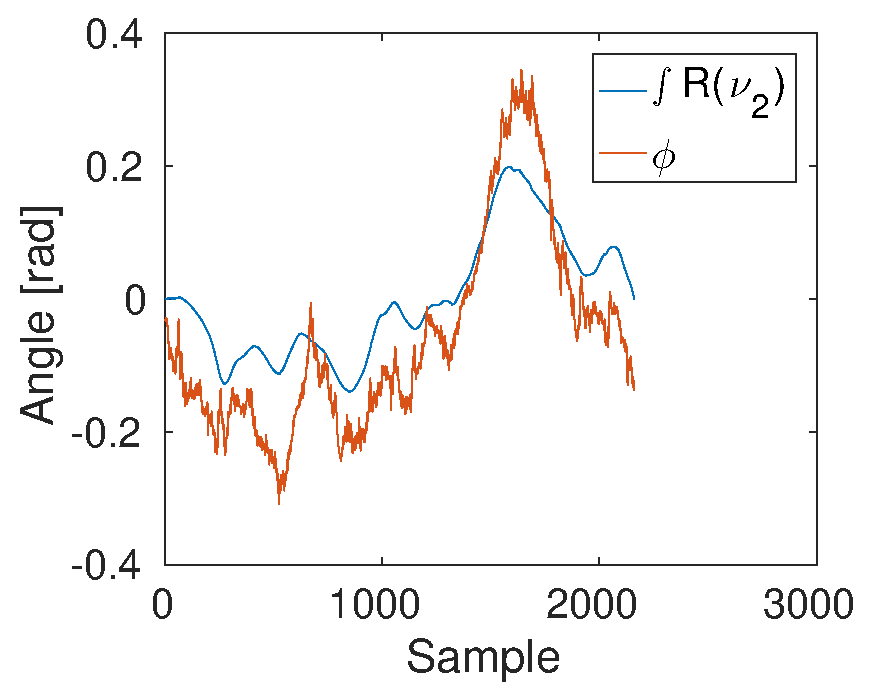
\includegraphics[width=0.5\textwidth]{velocityAnglePhi}}
  \qquad
  \subfloat[][\label{fig:velocityAngleTheta}A comparison between integrated angular velocities transformed to the global frame (blue) and the estimated angle \pitchAngle (red).]{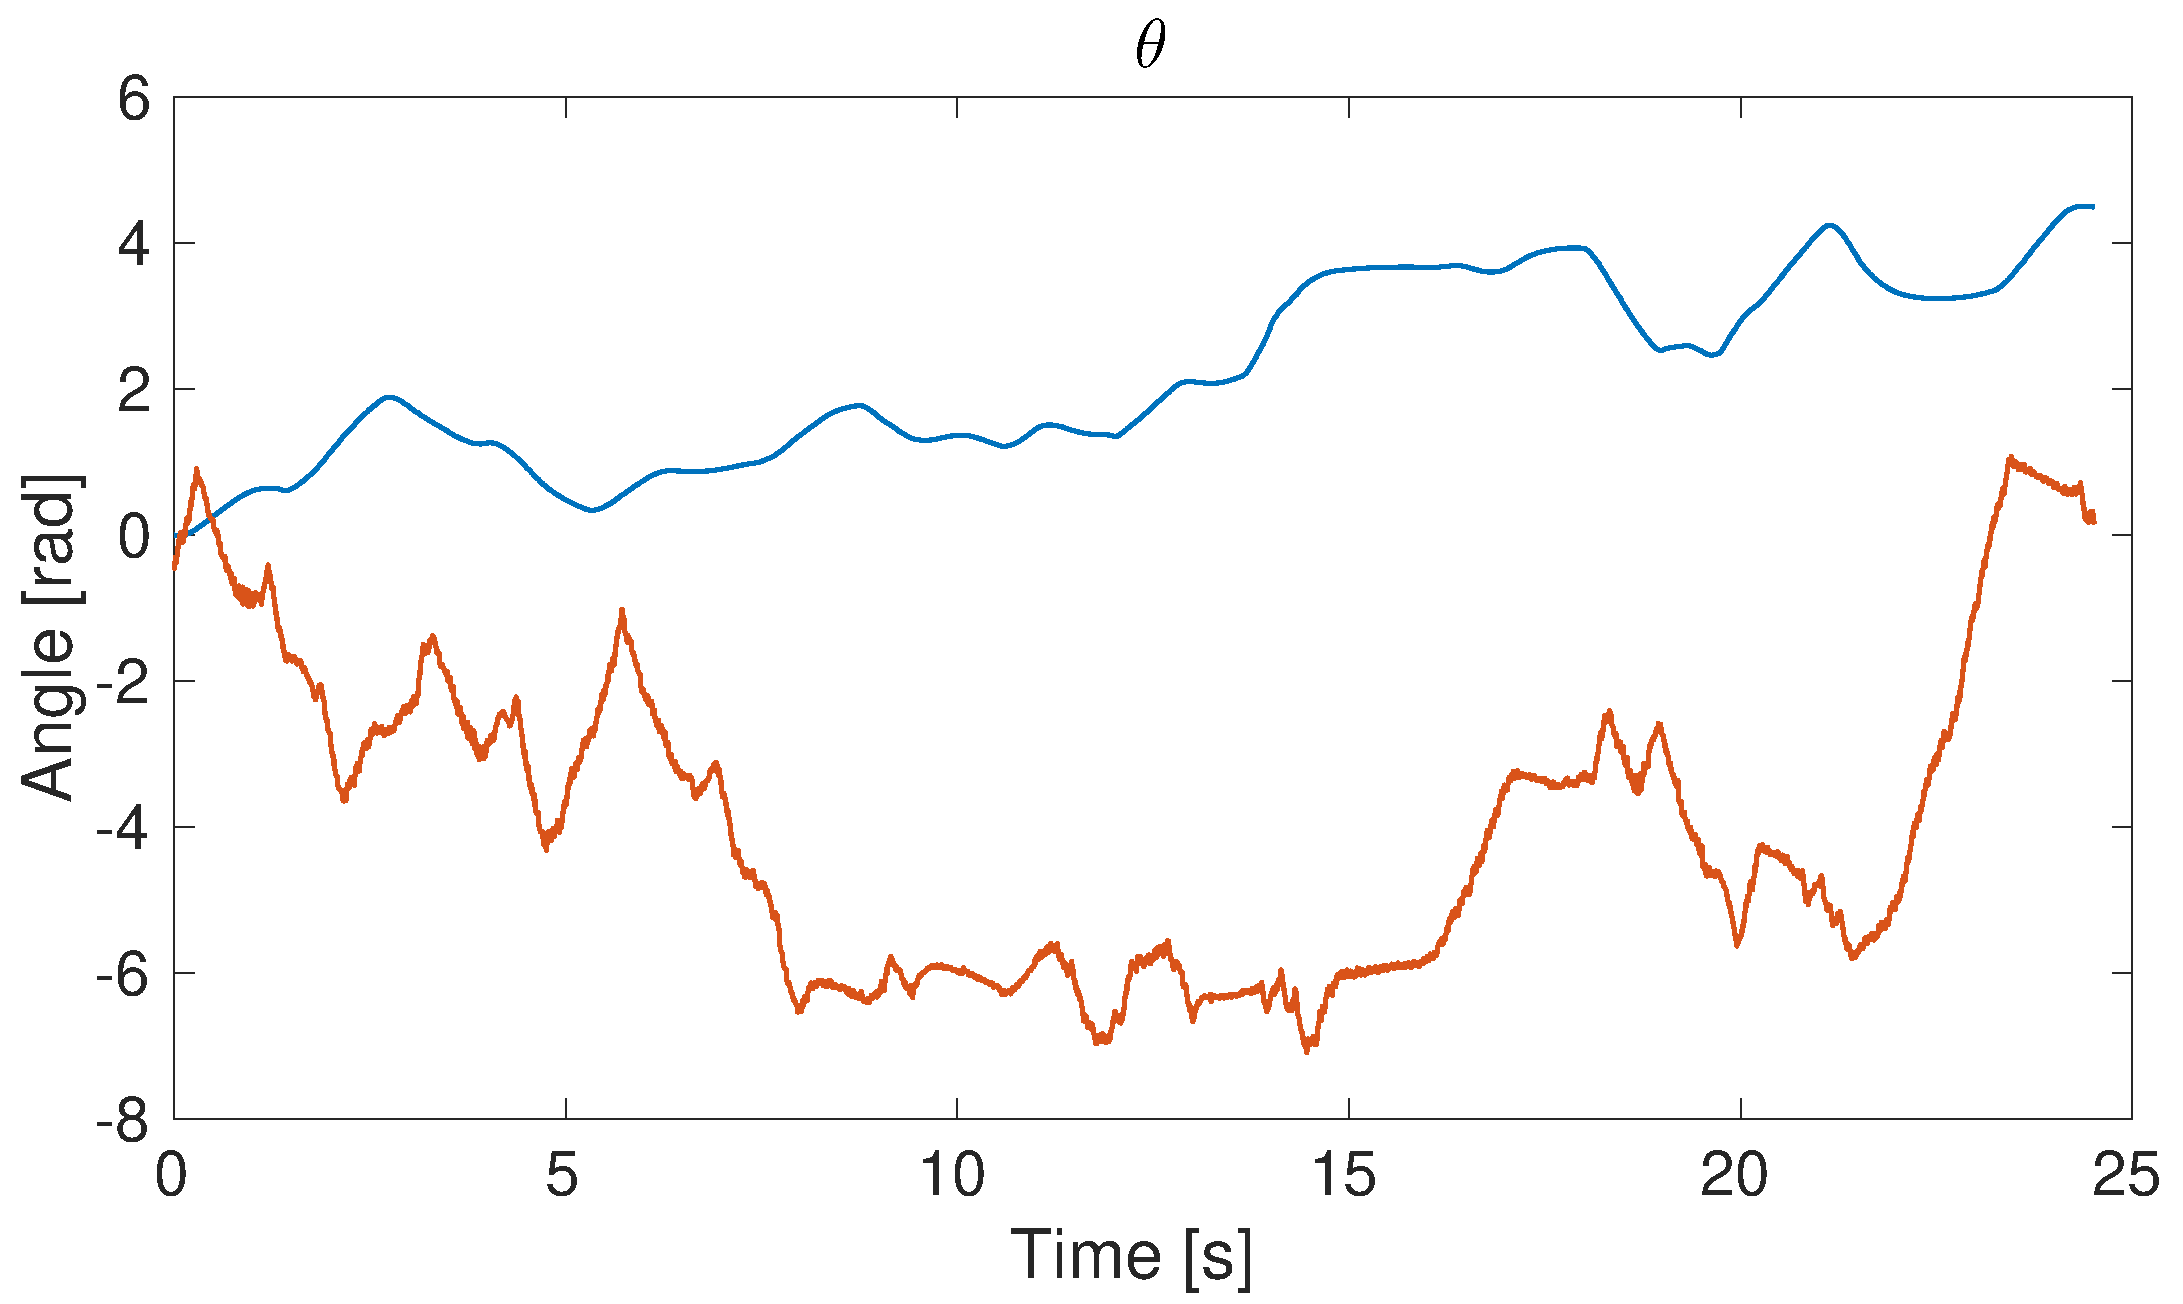
\includegraphics[width=0.5\textwidth]{velocityAngleTheta}}
  \\
  \subfloat[][\label{fig:velocityAnglePsi}A comparison between integrated angular velocities transformed to the global frame (blue) and the estimated angle \yawAngle (red).]{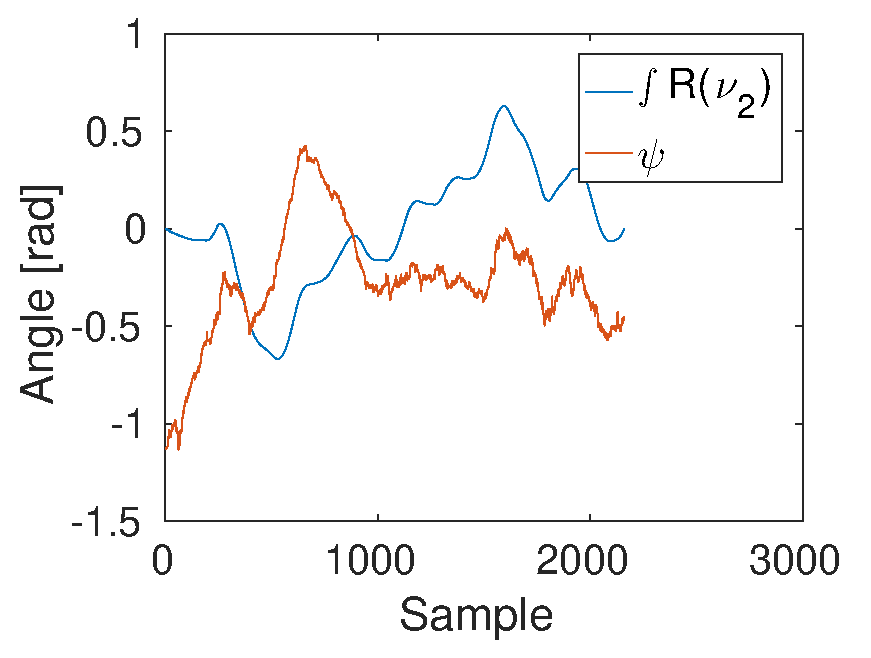
\includegraphics[width=0.5\textwidth]{velocityAnglePsi}}
  \caption{\label{fig:integratedAngleVelocities}%
    As can be seen in \protect\subref{fig:velocityAnglePhi}-\protect\subref{fig:velocityAnglePsi} the angles are poorly estimated and thus not suitable to use in parameter estimation. The angles are estimated with the method used in \Sectionref{sec:simple_model}.}
\end{figure}

To get an initial estimate on the parameters in the yaw dynamics the reduced model parameters in \eqref{eq:r_dot_simple}
were estimated. The estimation was done with data collected from a test that mainly excited the \abbrROV in $r$ and thus the cross-terms could be assumed to be zero.

The roll and pitch dynamics are coupled thus was \eqref{eq:pq_dot_simple} and \eqref{eq:pq_dot_simple2} estimated at the same time.
The cross terms could be assumed to be zero due since the \abbrROV was mainly excited in $p$ and $q$ during collection of the used estimation data.

The estimate of the parameters in \eqref{eq:r_dot_simple} and \eqref{eq:pq_dot_simple} was used as initial estimates of the parameters in \eqref{eq:q_dotWithoutTranslation}-\eqref{eq:r_dotWithoutTranslation}. Due to observational problems the reparametrisation $A_p = \Ix - \Kpdot$, $B_q = \Iy - \Mqdot$ and $C_r = \Iz - \Nrdot$ was done. In \Figureref{fig:velocityCompare} the simulated model without reparametrisation can be seen. An improvement of the fit can be seen in \Figureref{fig:velocityCompareCong} where some parameters has been reparameterised.
\index{Reduced model structure}
\begin{figure}[tbp]
  \centering
  \subfloat[][\label{fig:velocityComparep}Comparison between a simulated model without reparametrisation and validation data in $p$.]{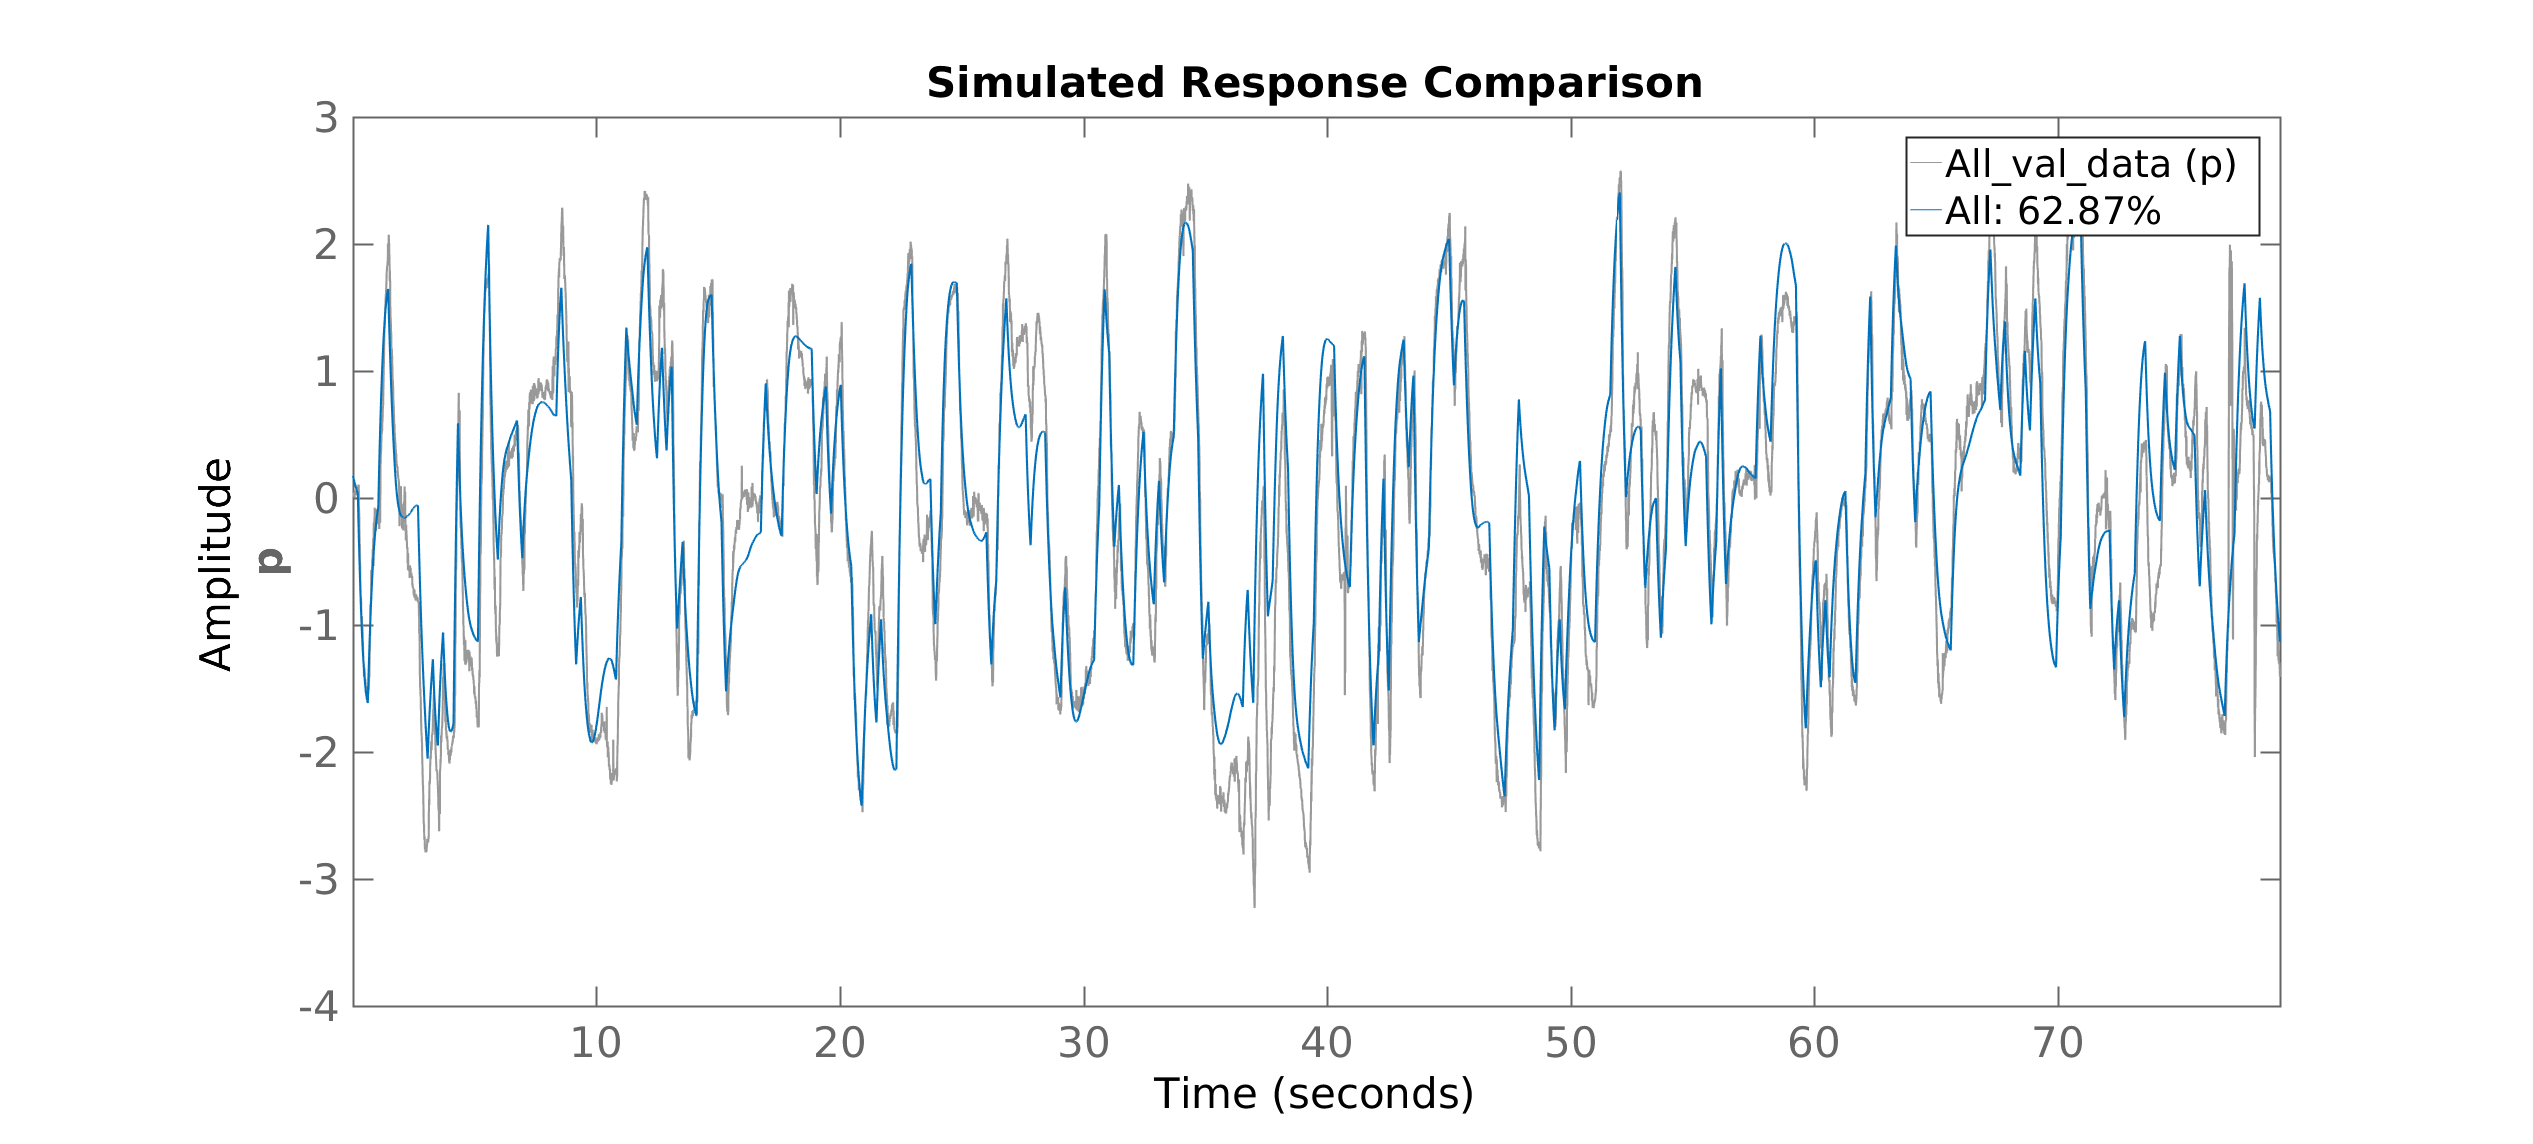
\includegraphics[width=0.8\textwidth]{velocityComparep}}
  \qquad
  \subfloat[][\label{fig:velocityCompareq}Comparison between a simulated model without reparametrisation and validation data in the $q$.]{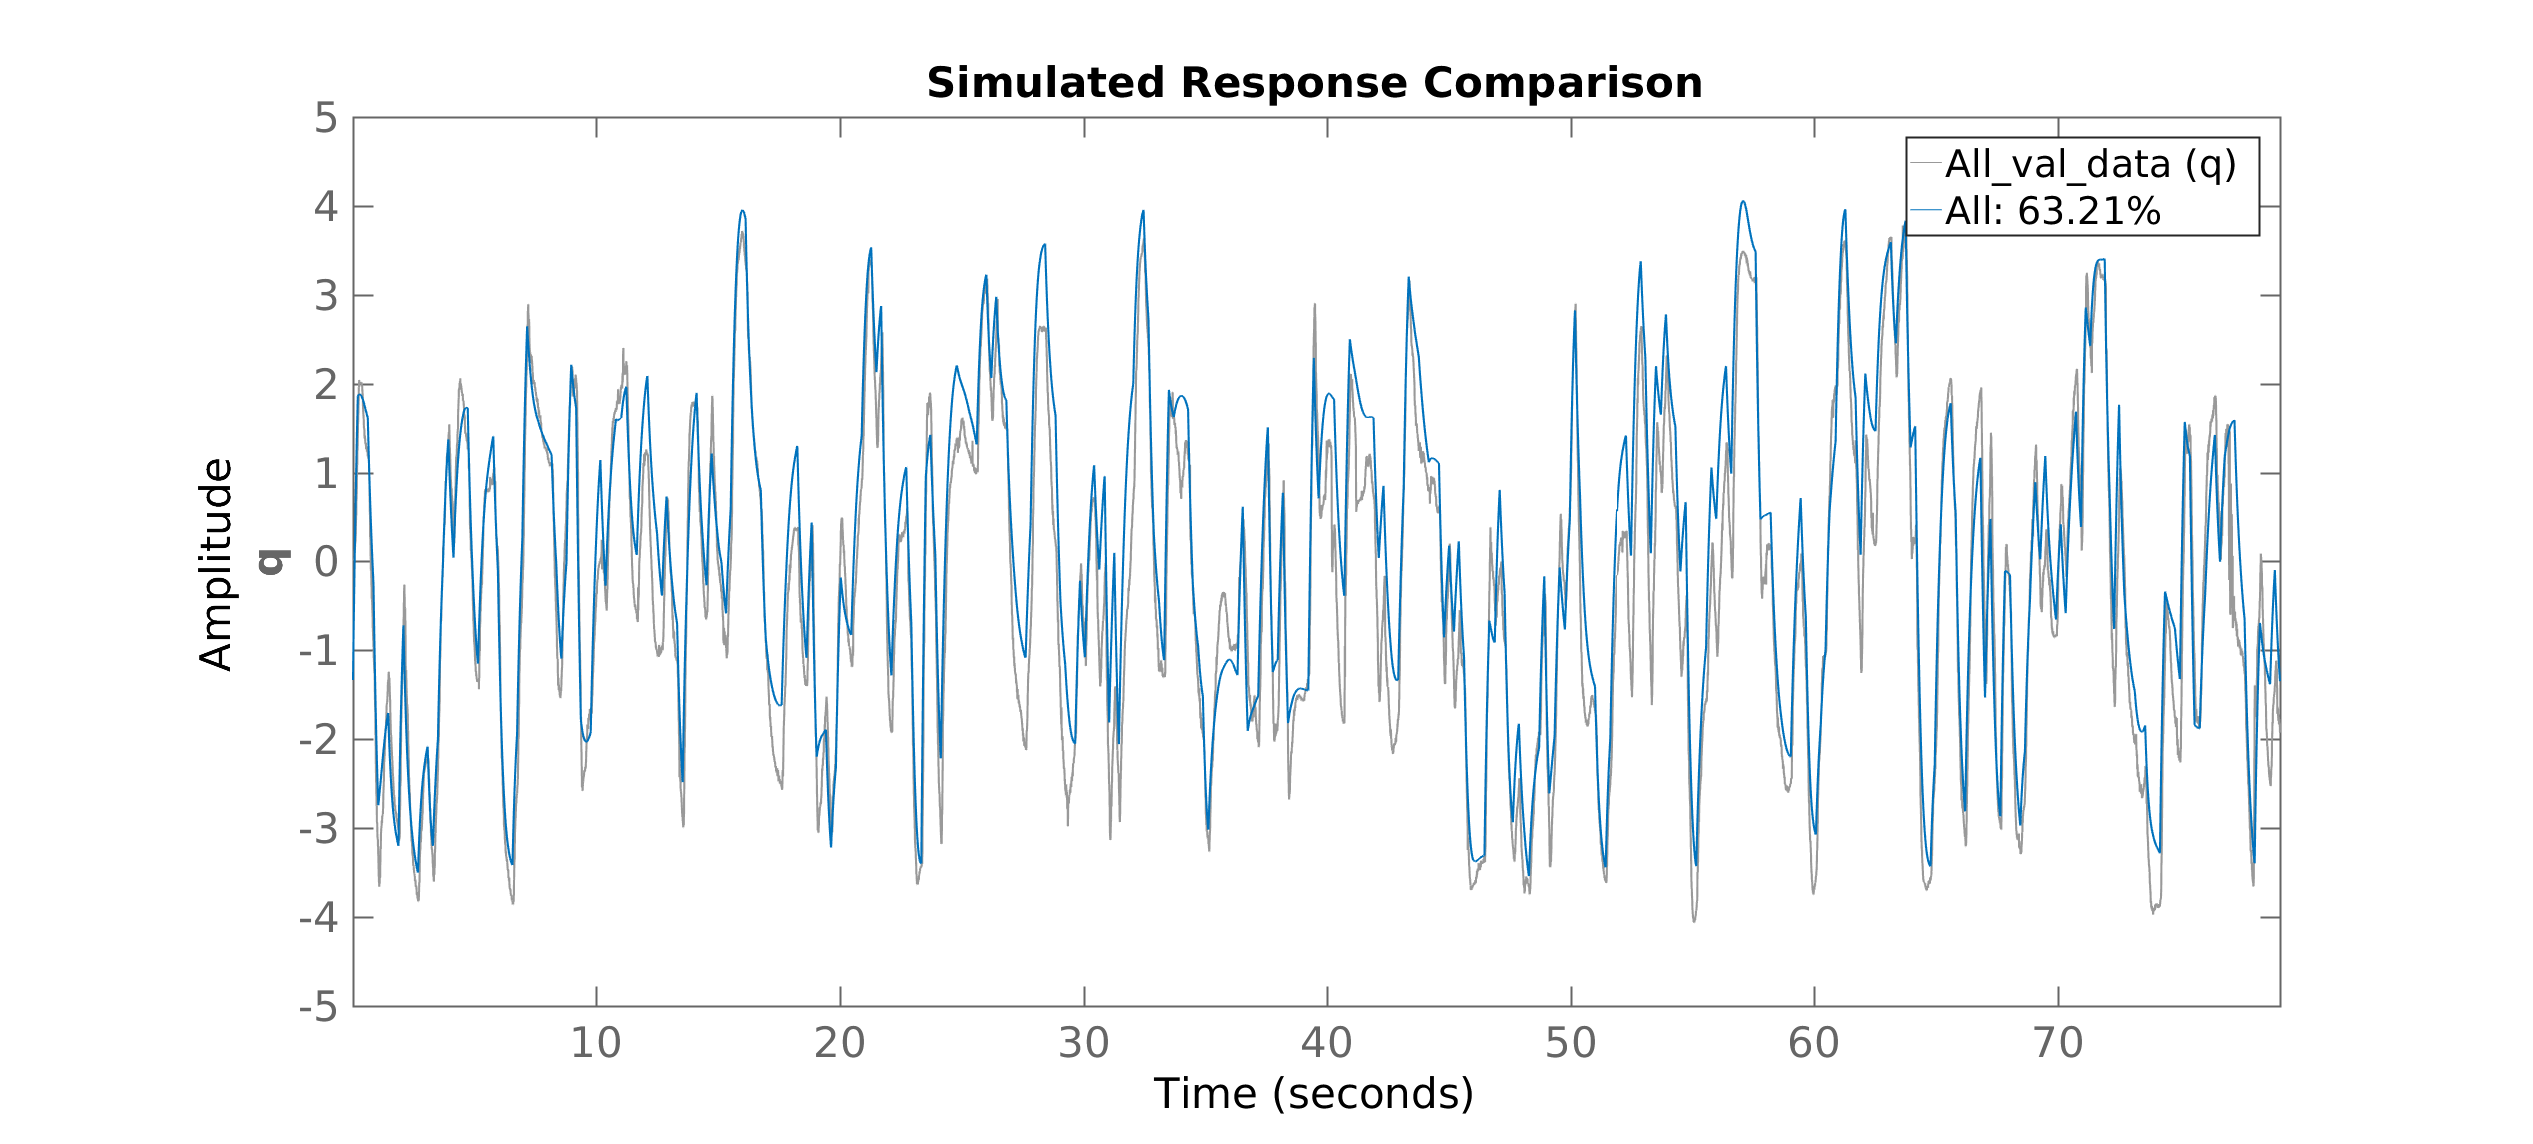
\includegraphics[width=0.8\textwidth]{velocityCompareq}}
  \\
  \subfloat[][\label{fig:velocityComparer}Comparison between a simulated model without reparametrisation and validation data in the $r$.]{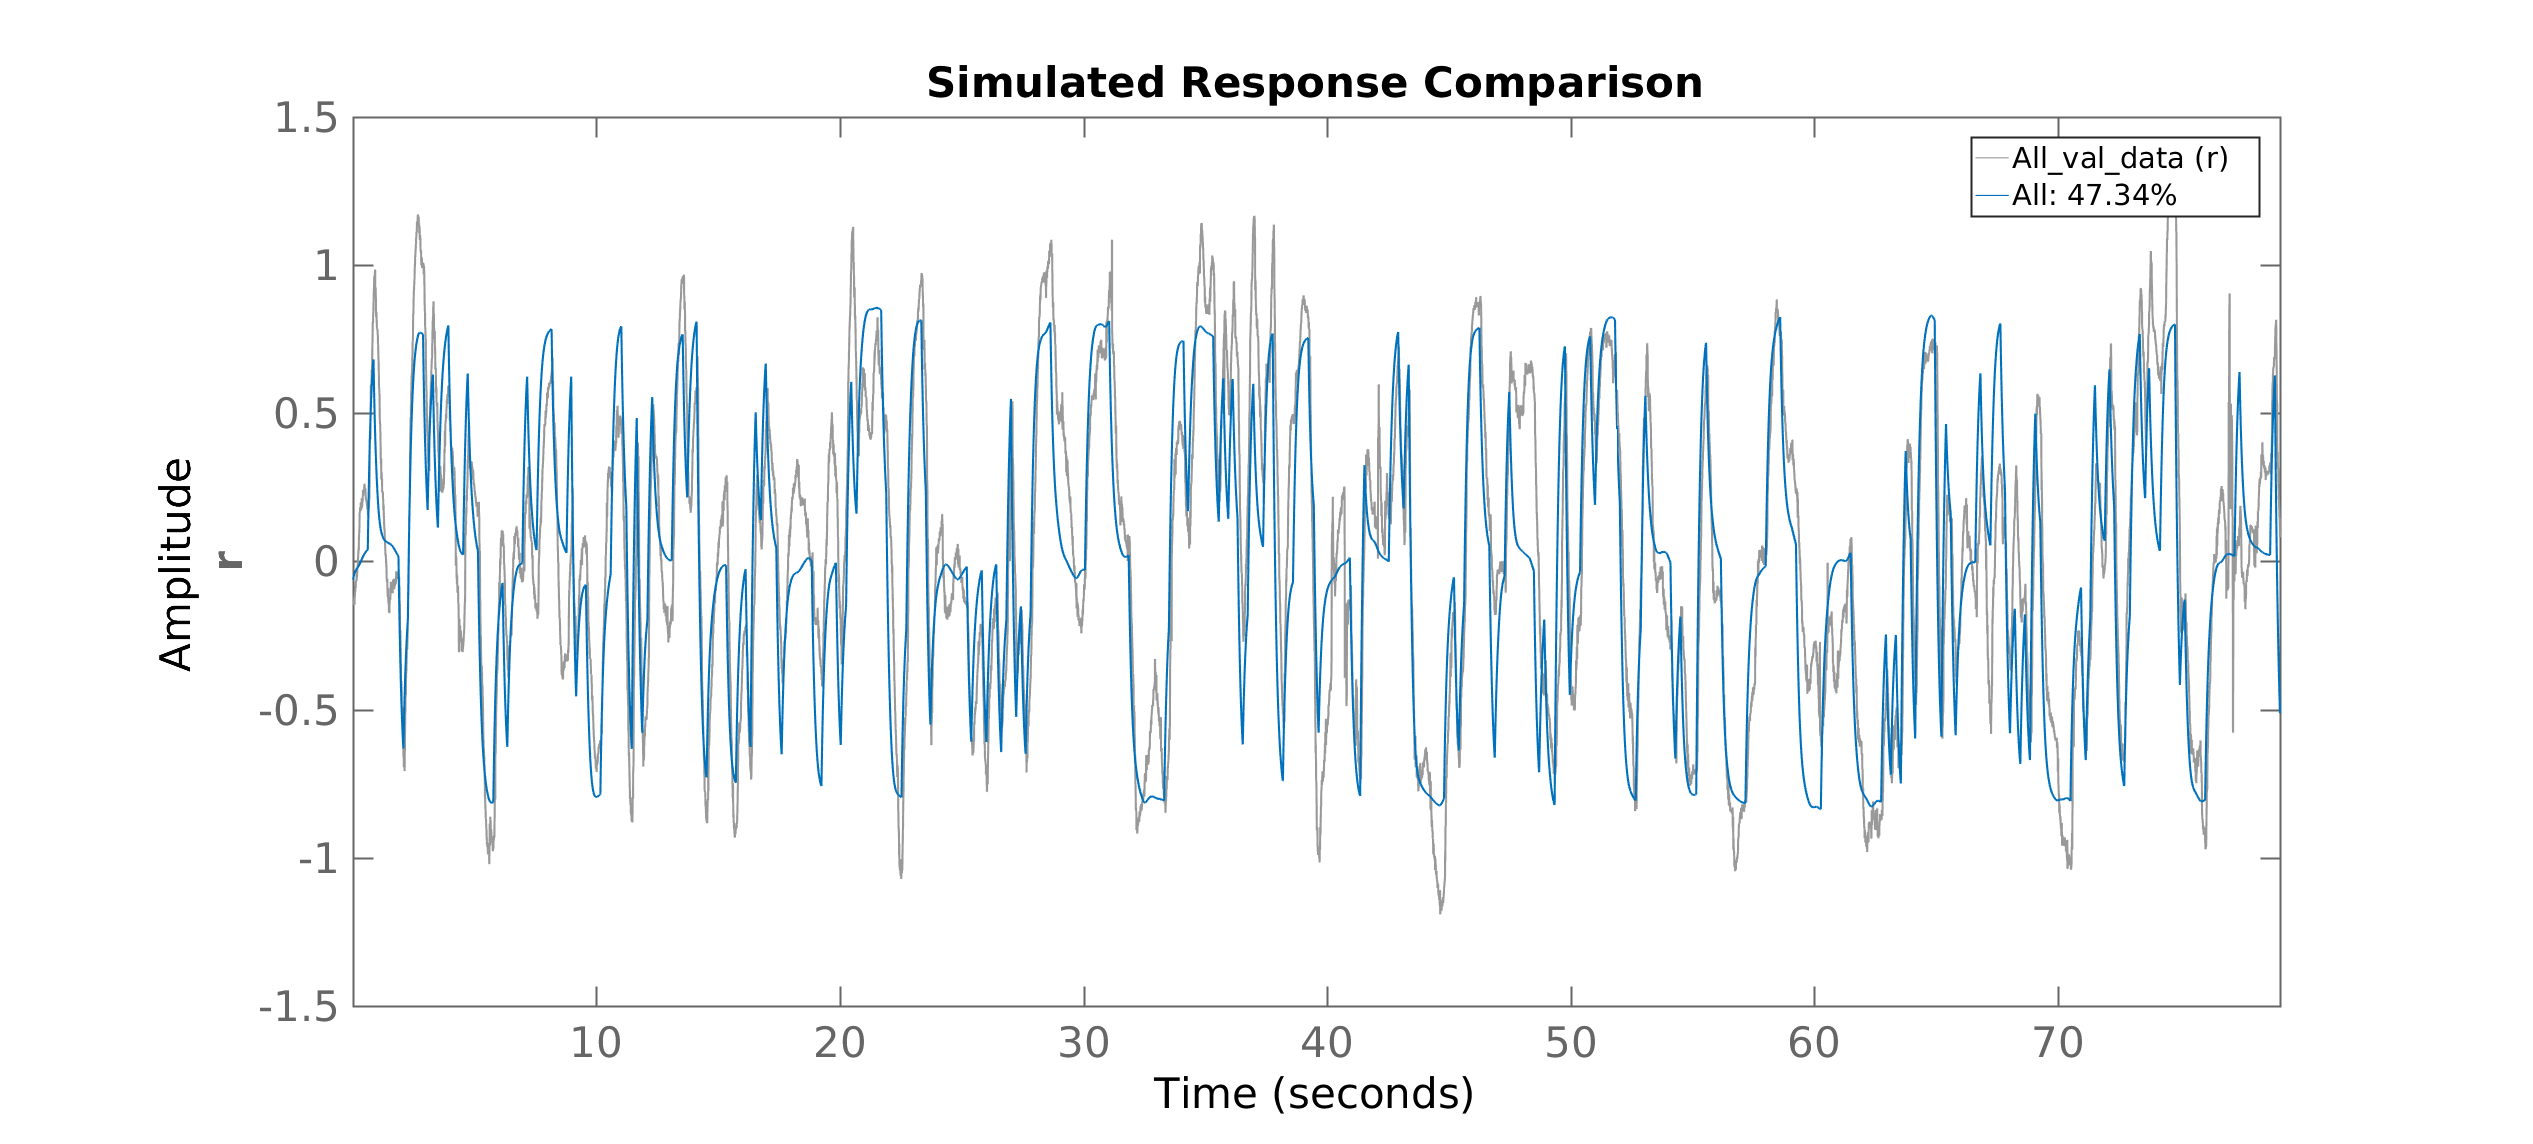
\includegraphics[width=0.8\textwidth]{velocityComparer}}
  \caption{\label{fig:velocityCompare}%
    Comparison between simulation of the attitude model and validation data.}
\end{figure}

\begin{figure}[tbp]
  \centering
  \subfloat[][\label{fig:velocityCompareCongp}Comparison between a simulated model without reparametrisation and validation data in the $p$.]{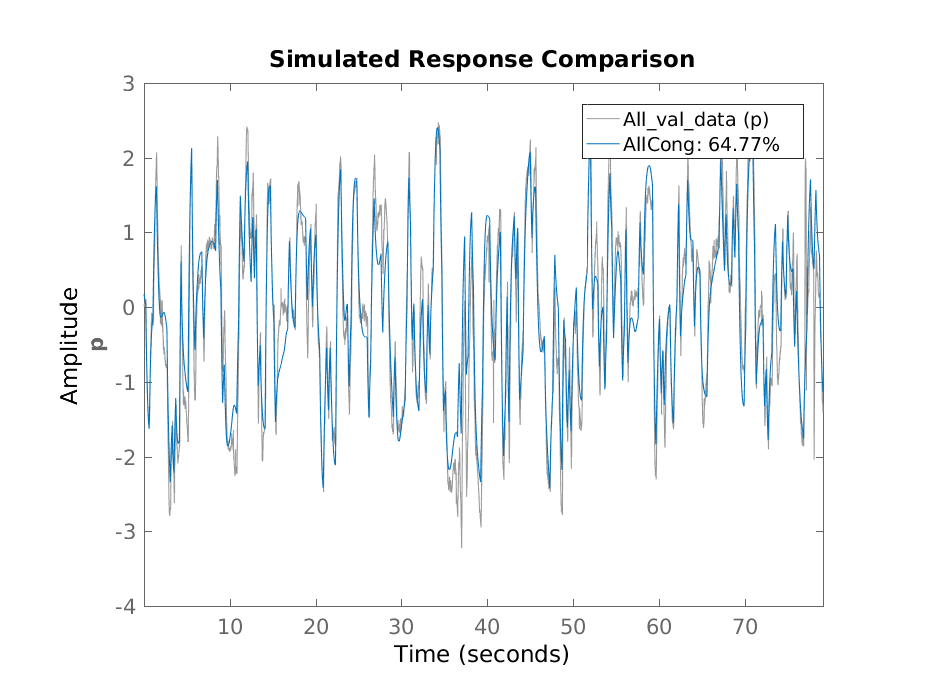
\includegraphics[width=0.5\textwidth]{velocityCompareCongp}}
  \qquad
  \subfloat[][\label{fig:velocityCompareCongq}Comparison between a simulated model without reparametrisation and validation data in the $q$.]{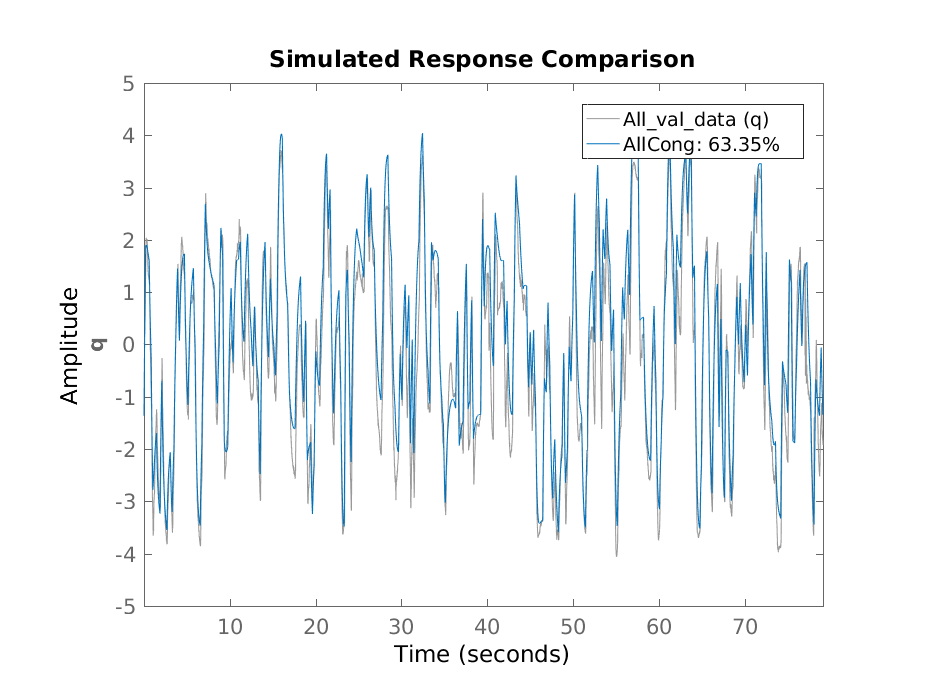
\includegraphics[width=0.5\textwidth]{velocityCompareCongq}}
  \\
  \subfloat[][\label{fig:velocityCompareCongr}Comparison between a simulated model without reparametrisation and validation data in the $r$.]{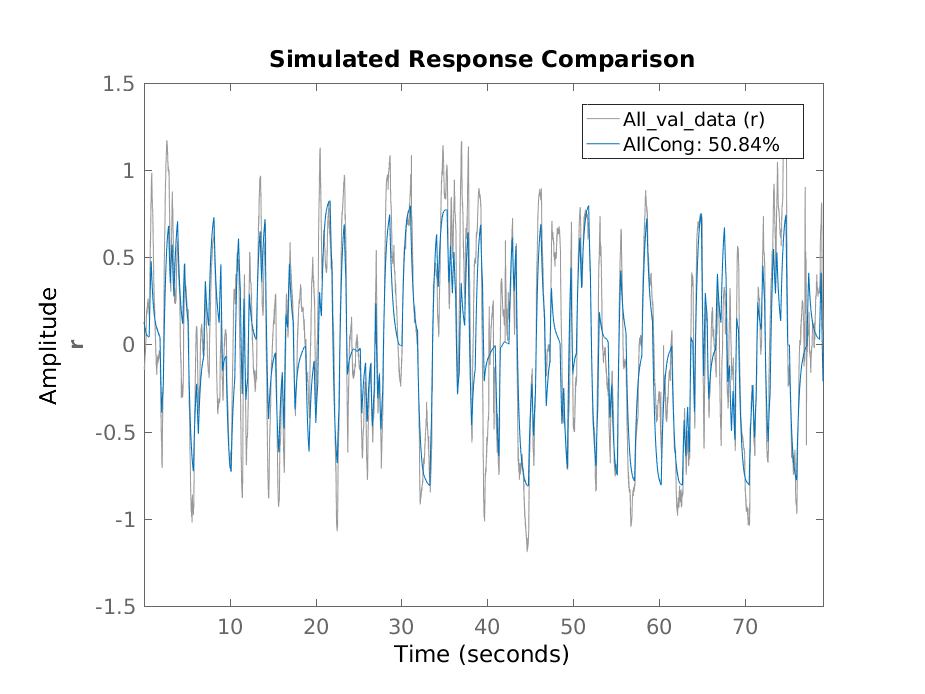
\includegraphics[width=0.5\textwidth]{velocityCompareCongr}}
  \caption{\label{fig:velocityCompareCong}%
    Comparison of simulation of the attitude model against validation data.}
\end{figure}

%%%%%%%%%%%%%%%%%%%%%%%%%%%%%%%%%%%%%%%%%%%%%%%%%%%%%%%%%%%
\section{Parameter Estimation from Angular Velocities and Linear Acceleration} \label{sec:angLinEstim}
The parameters were also estimated using the angular velocities and the linear accelerations as outputs. This was done to bypass the low-pass filtering effects from the sensor fusion described in \Chapterref{cha:sensor_fusion}. The model structure was modified to use quaternions instead of euler angles. Using quaternions in the model \eqref{eq:p_dotWithoutTranslation} - \eqref{eq:r_dotWithoutTranslation} with the reparameterision from \Sectionref{sec:estimation_angular} gave the following model structure
\begin{multline}
\pdot = \frac{\thrusterfun{1} \distance{y}{1} - \thrusterfun{2} \distance{y}{2} + \thrusterfun{6} \distance{z}{6}}{A_p} + \frac{B z_B (2 \quatII \quatIII + 2 \quatI \quatO)}{A_p} + \\ \frac{p (\Kp + \Kpabsp \abs(p))}{A_p} + \frac{q r (B_q - C_r)}{A_p},
\end{multline}
\begin{multline}
\qdot = \frac{\thrusterfun{1} \distance{x}{1} + \thrusterfun{2} \distance{x}{2} - \thrusterfun{5} \distance{x}{5}}{B_q} - \frac{B z_B (2 \quatI \quatIII - 2 \quatII \quatO)}{B_q} + \\ \frac{q (\Mq + \Mqabsq \abs(q))}{B_q} - \frac{p r (A_p - C_r)}{B_q}
\end{multline}
and
\begin{multline}
\rdot = \frac{\thrusterfun{3} \distance{y}{3} - \thrusterfun{4} \distance{y}{4}}{C_r} + \frac{r (\Nr + \Nrabsr \abs(r))}{C_r} + \frac{p q (A_p  - B_q)}{C_r}
\end{multline} was obtained.

The model structure in which the parameters was estimated became \index{model structure}
\begin{equation}
\etaVectordot = J(\etaVector) \nuVector,
\end{equation}
\begin{equation}
\dot{\nuVector} =  f(\etaVector, \nuVector, \tauVector)
\end{equation}
and
\begin{equation}
\boldsymbol{y} = \begin{pmatrix}
\etaVector \\
\boldsymbol{a}
\end{pmatrix}
\end{equation}
where $\boldsymbol{a}$ are the linear accelerations in the \abbrROV frame. 
\begin{figure}[tbp]
  \centering
  \subfloat[][\label{fig:angVelComparep}Comparison of angular velocity around the \abbrROV's x-axis between validation data and the simulated model.]{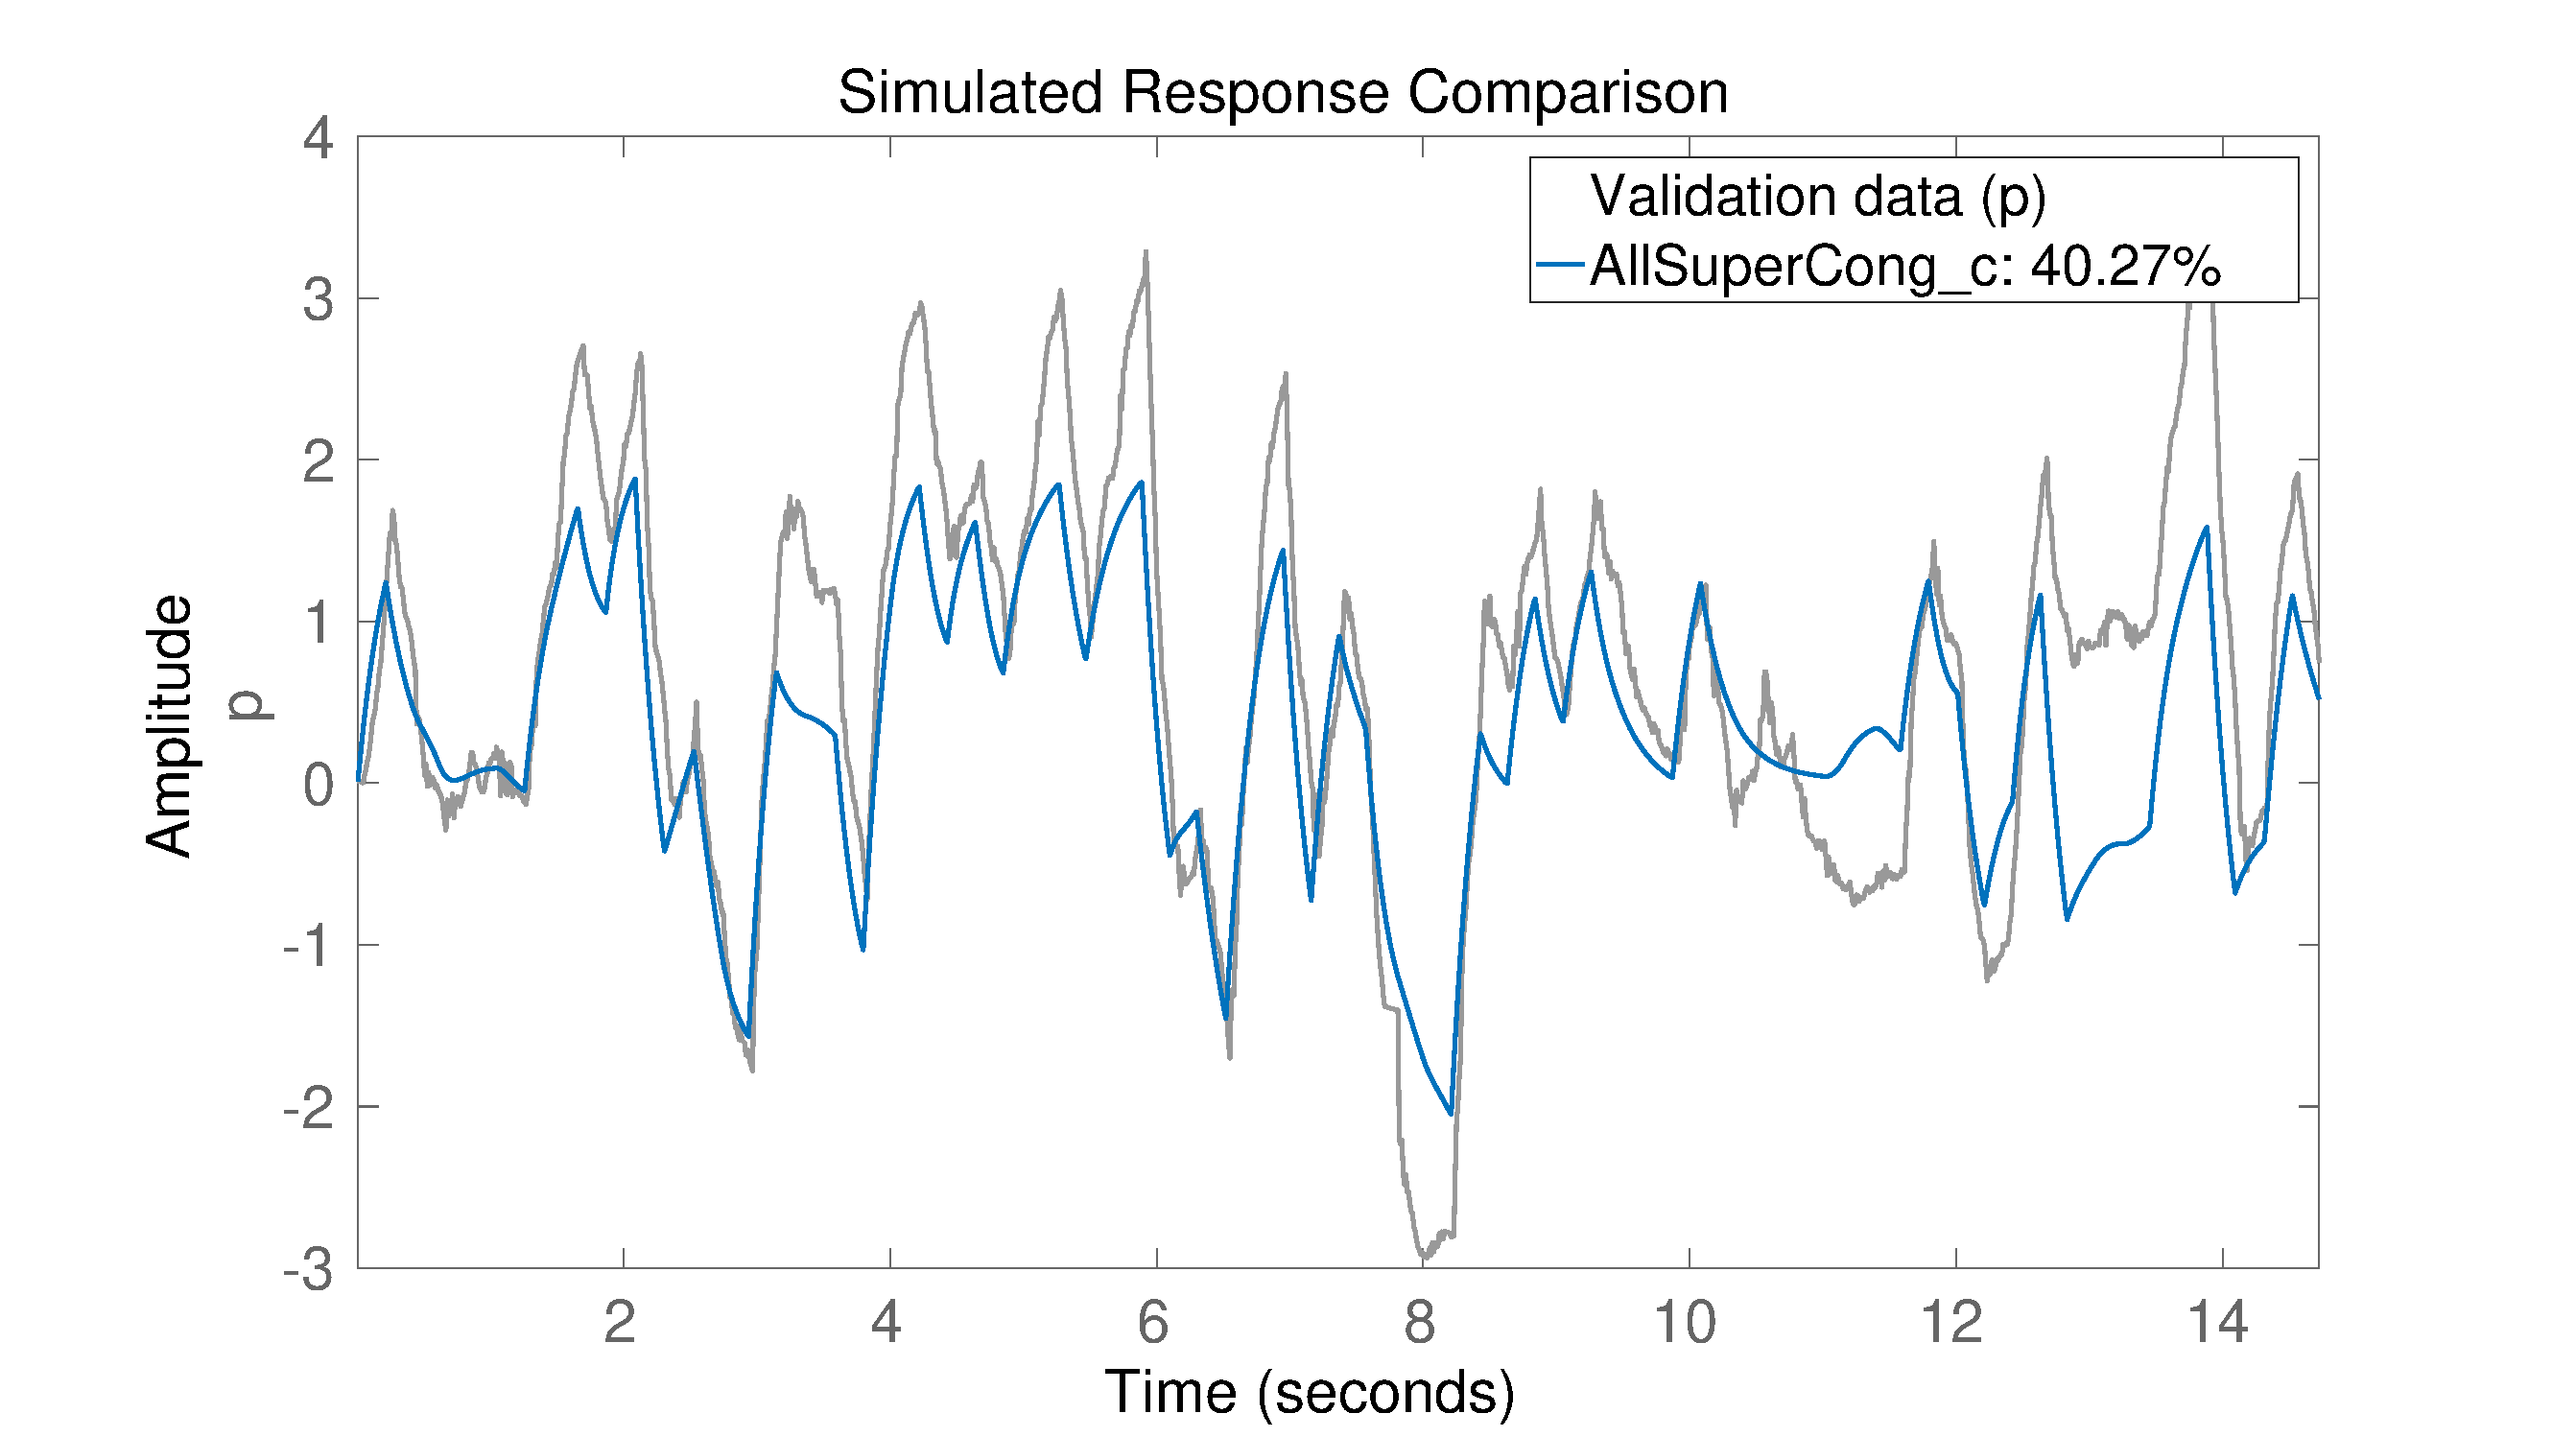
\includegraphics[width=0.4\textwidth]{angVelComparep}}
  \qquad
  \subfloat[][\label{fig:angVelCompareq}Comparison of angular velocity around the \abbrROV's y-axis between validation data and the simulated model.]{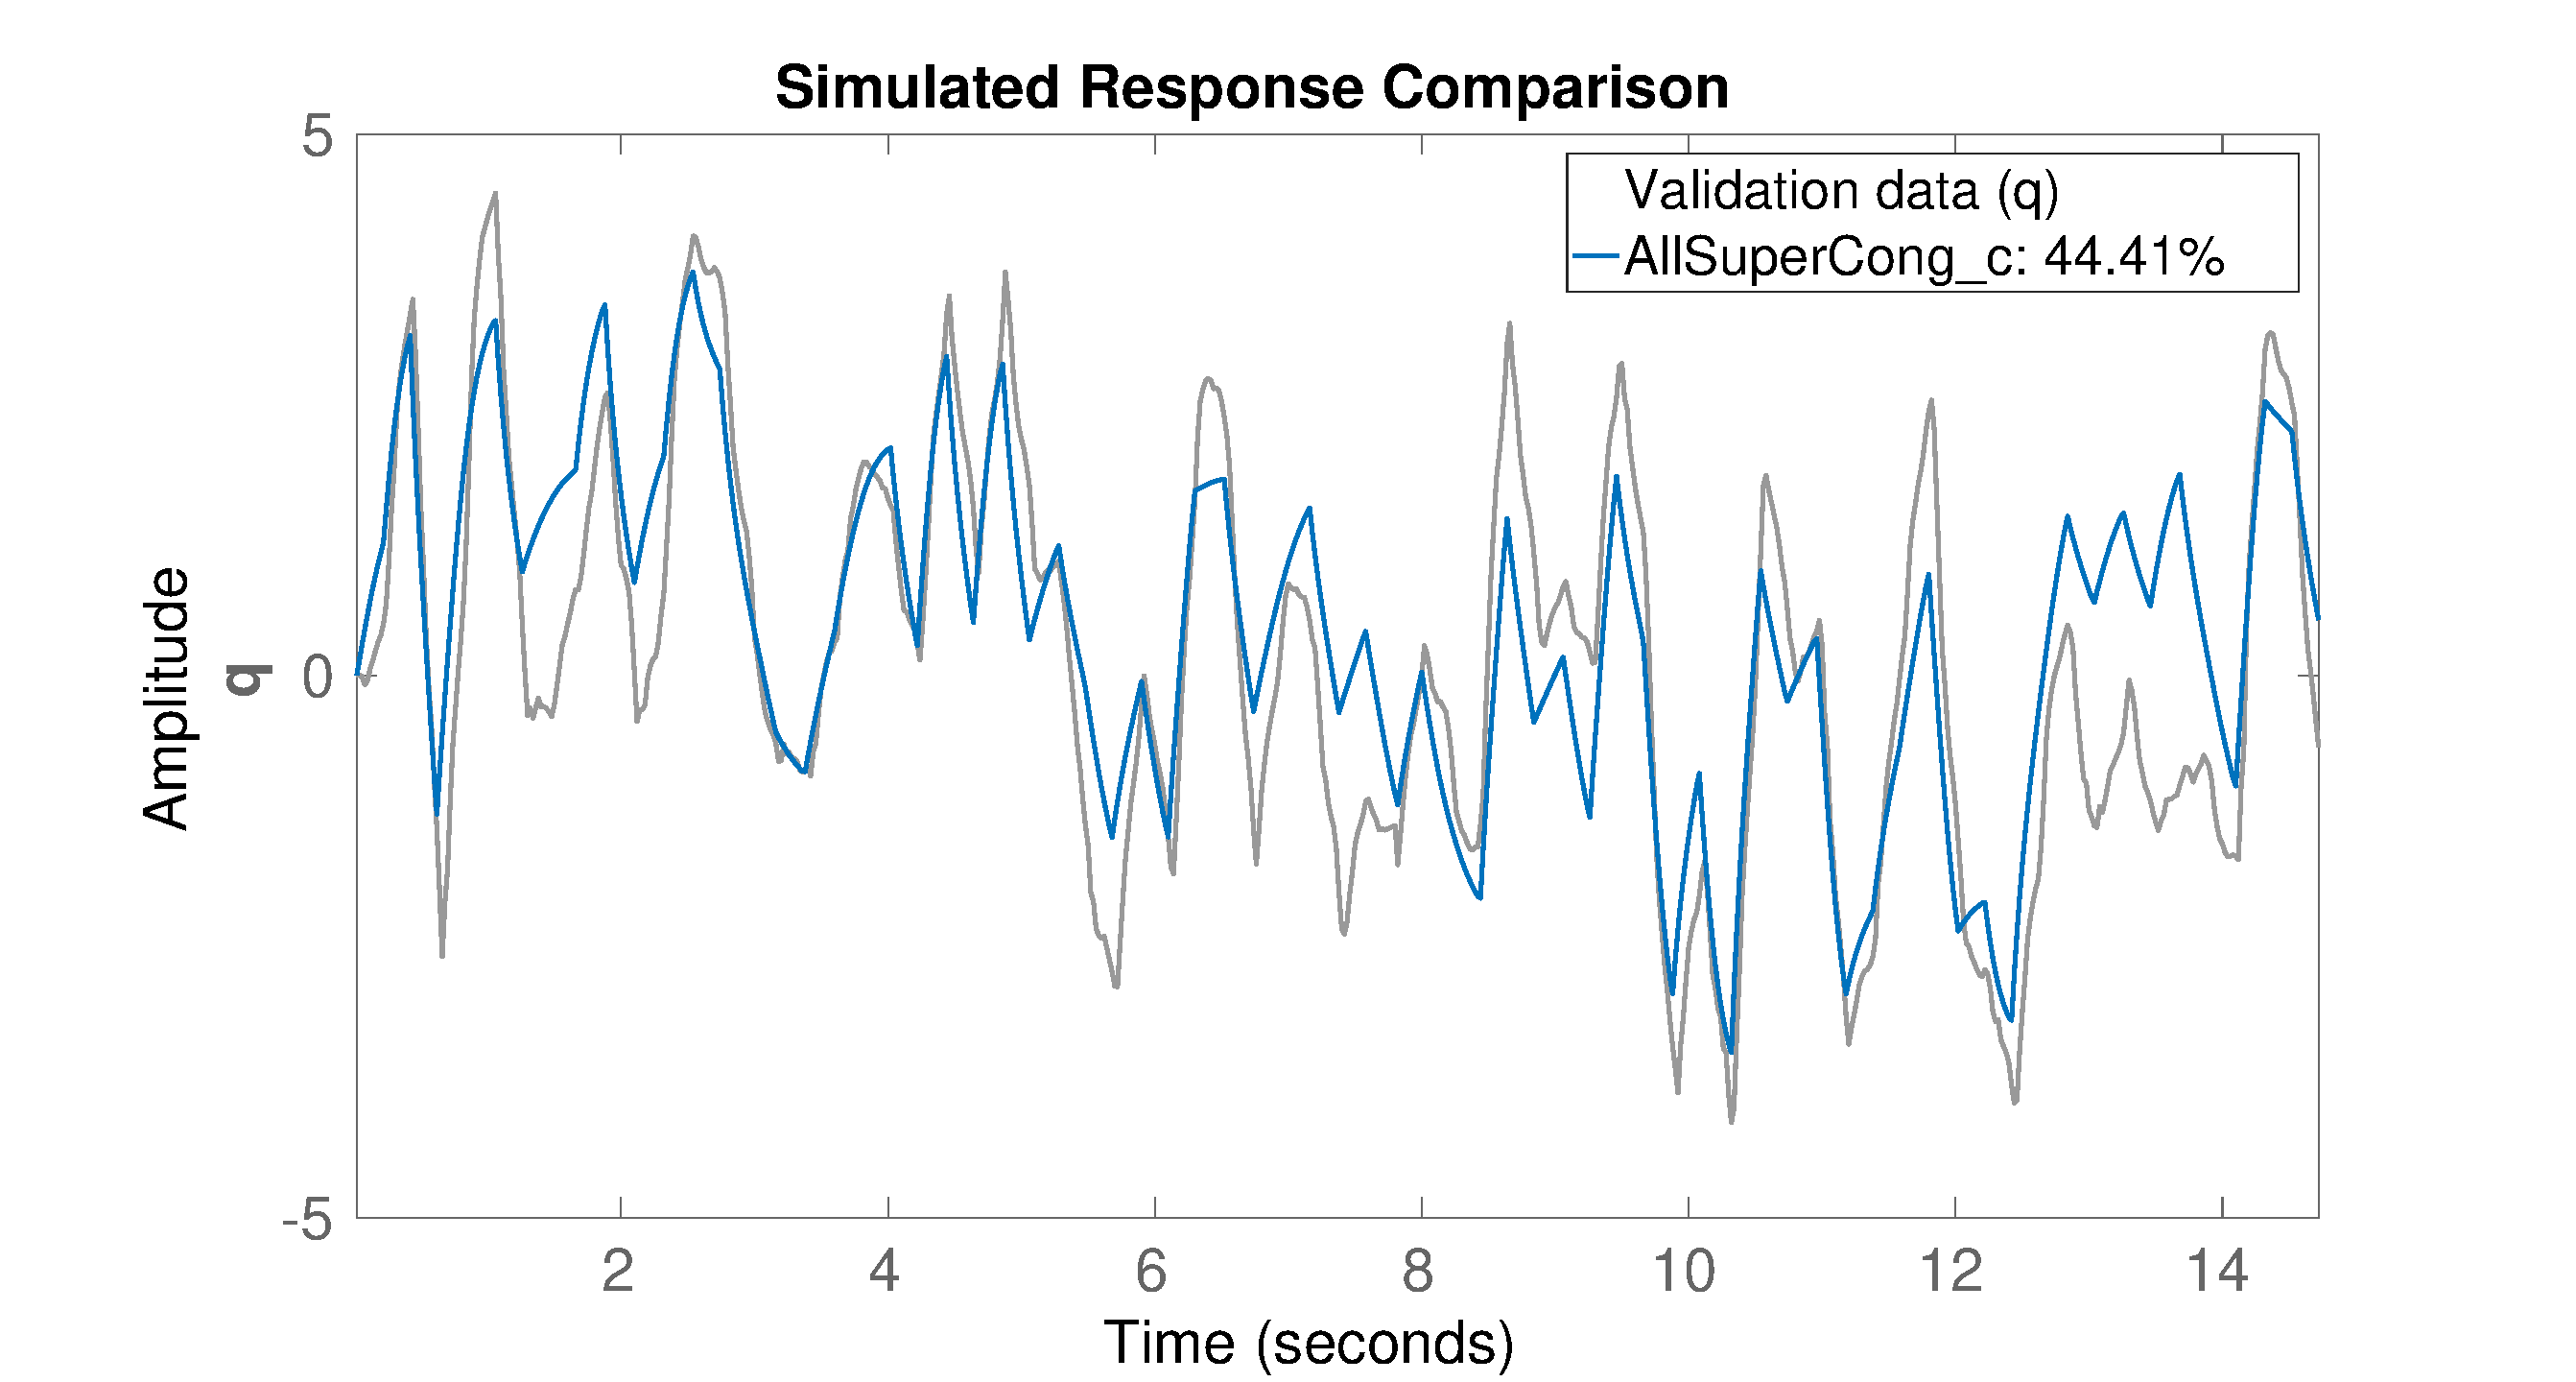
\includegraphics[width=0.4\textwidth]{angVelCompareq}}
  \qquad
  \subfloat[][\label{fig:angVelComparer}Comparison of angular velocity around the \abbrROV's z-axis between validation data and the simulated model.]{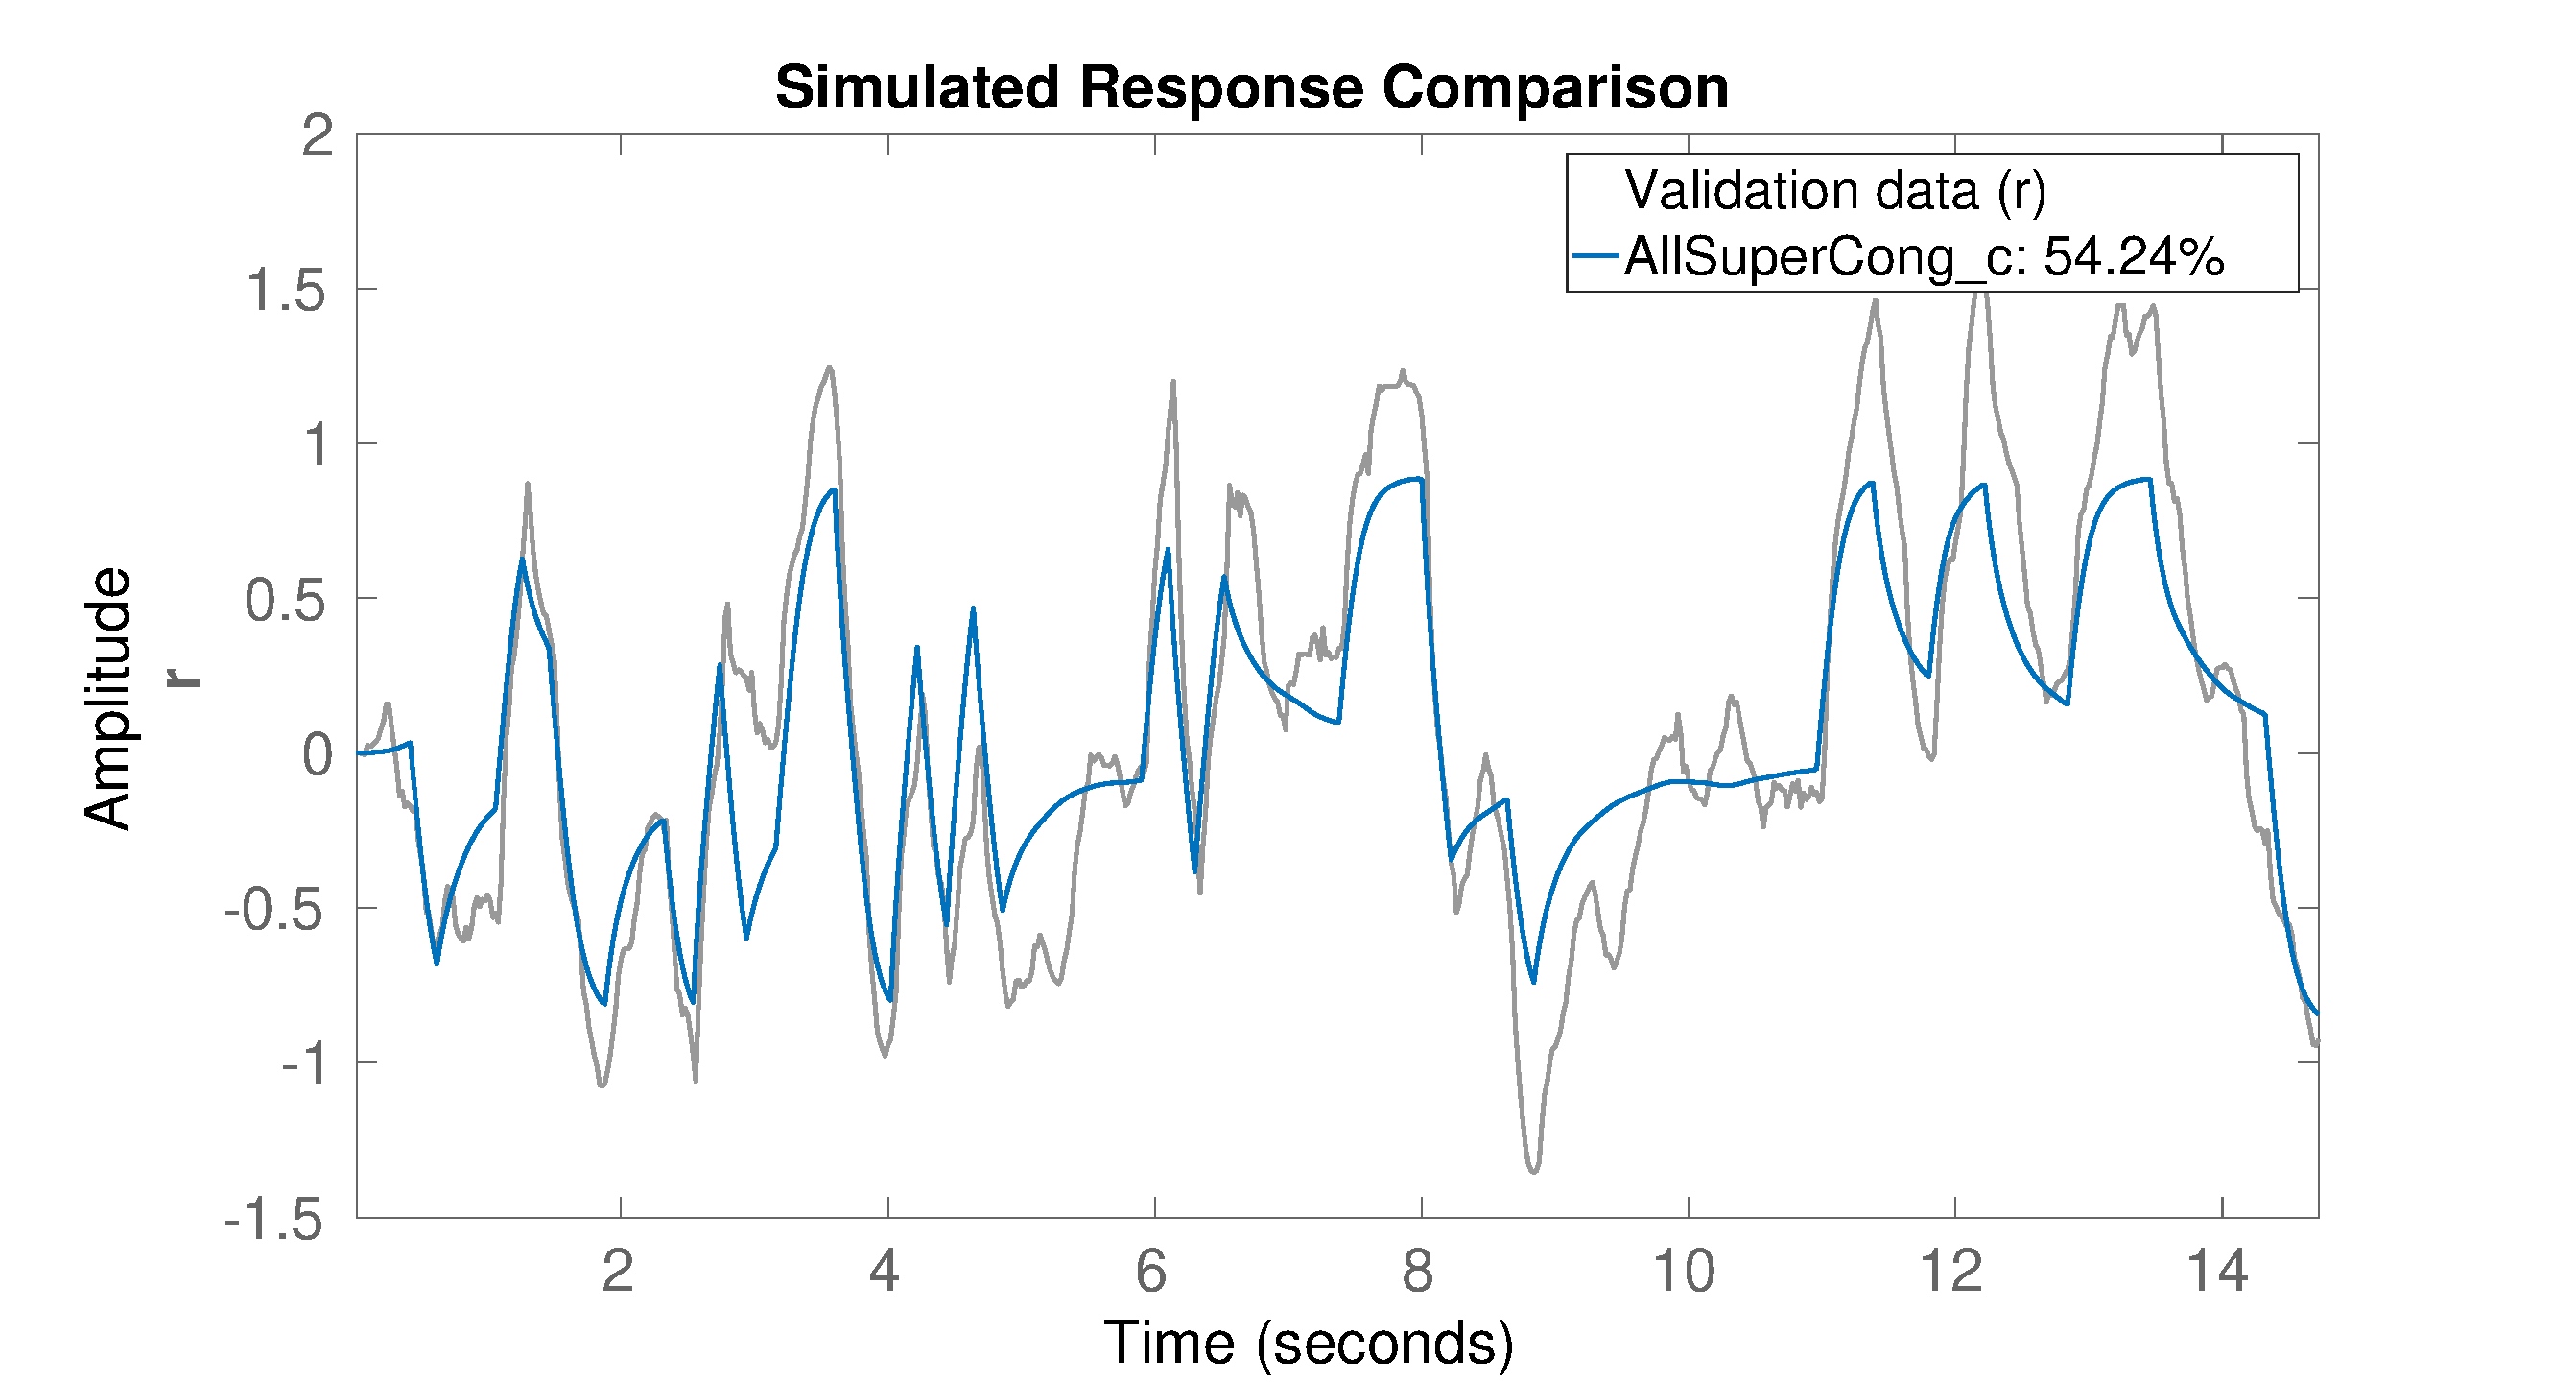
\includegraphics[width=0.4\textwidth]{angVelComparer}}
    \qquad
  \subfloat[][\label{fig:linAccComparex}Comparison of linear acceleration in the \abbrROV's x-axis between validation data and the simulated model.]{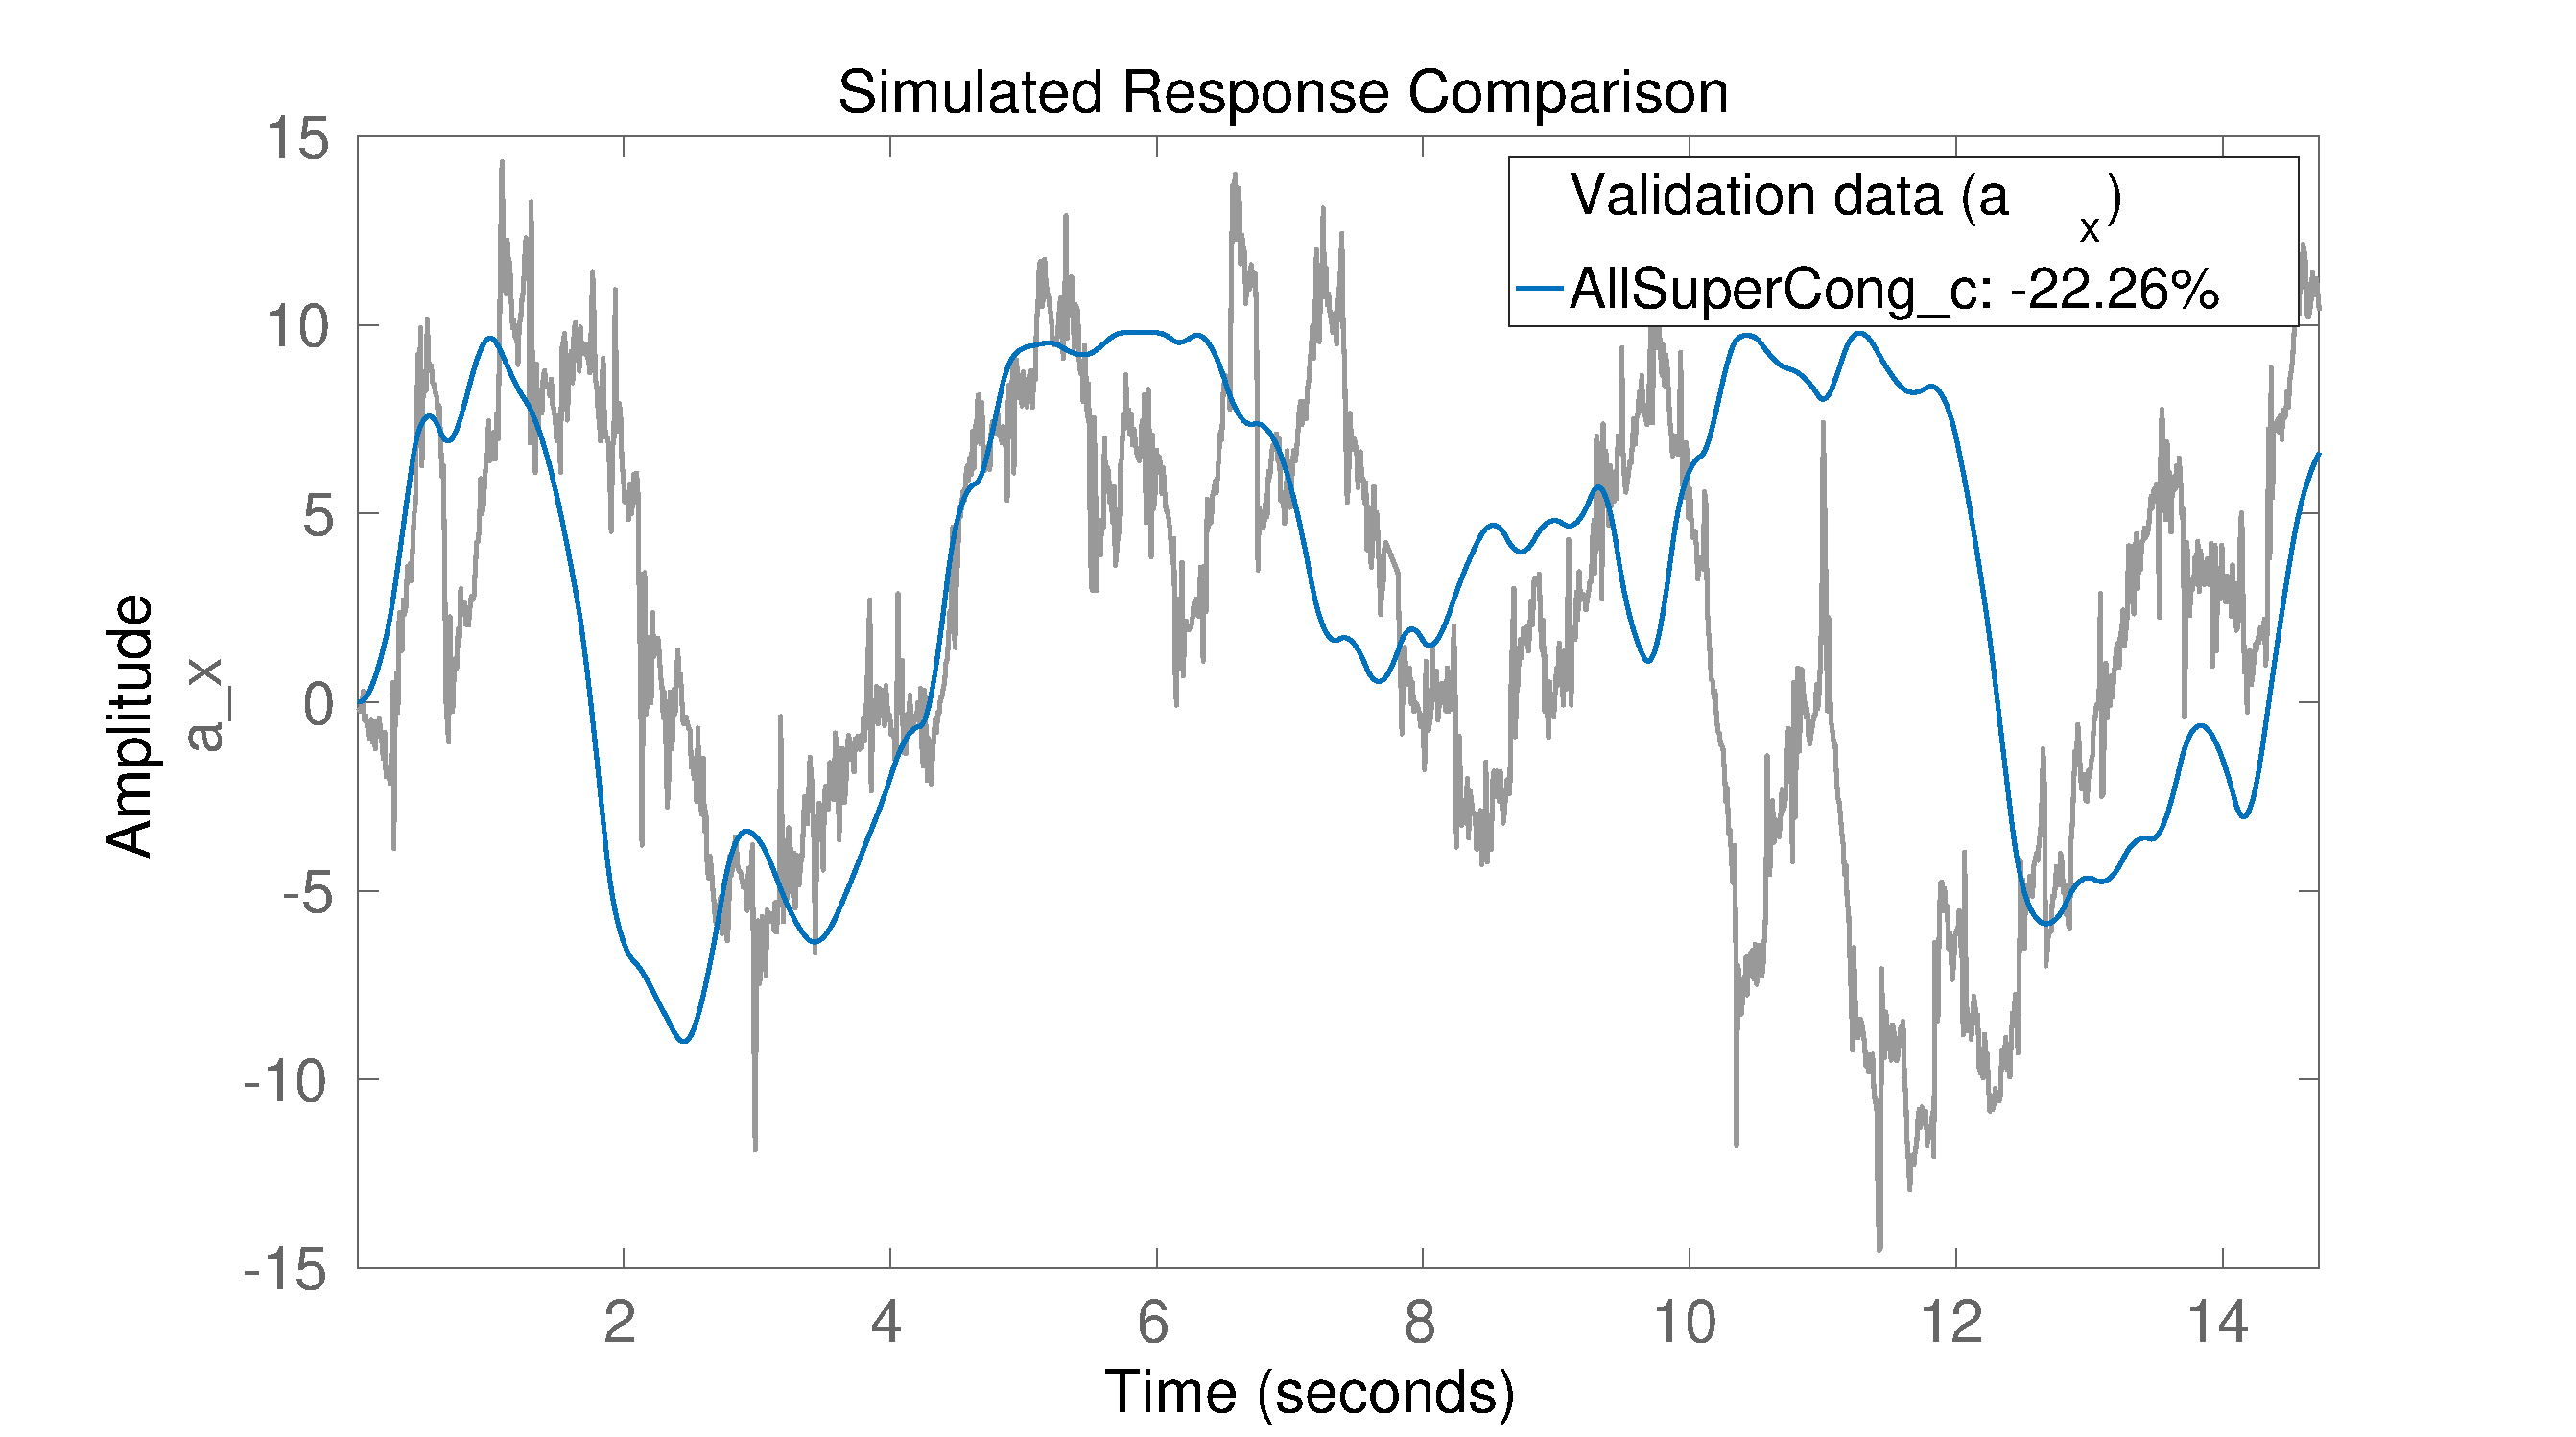
\includegraphics[width=0.4\textwidth]{linAccComparex}}
    \qquad
  \subfloat[][\label{fig:linAccComparey}Comparison of linear acceleration in the \abbrROV's y-axis between validation data and the simulated model.]{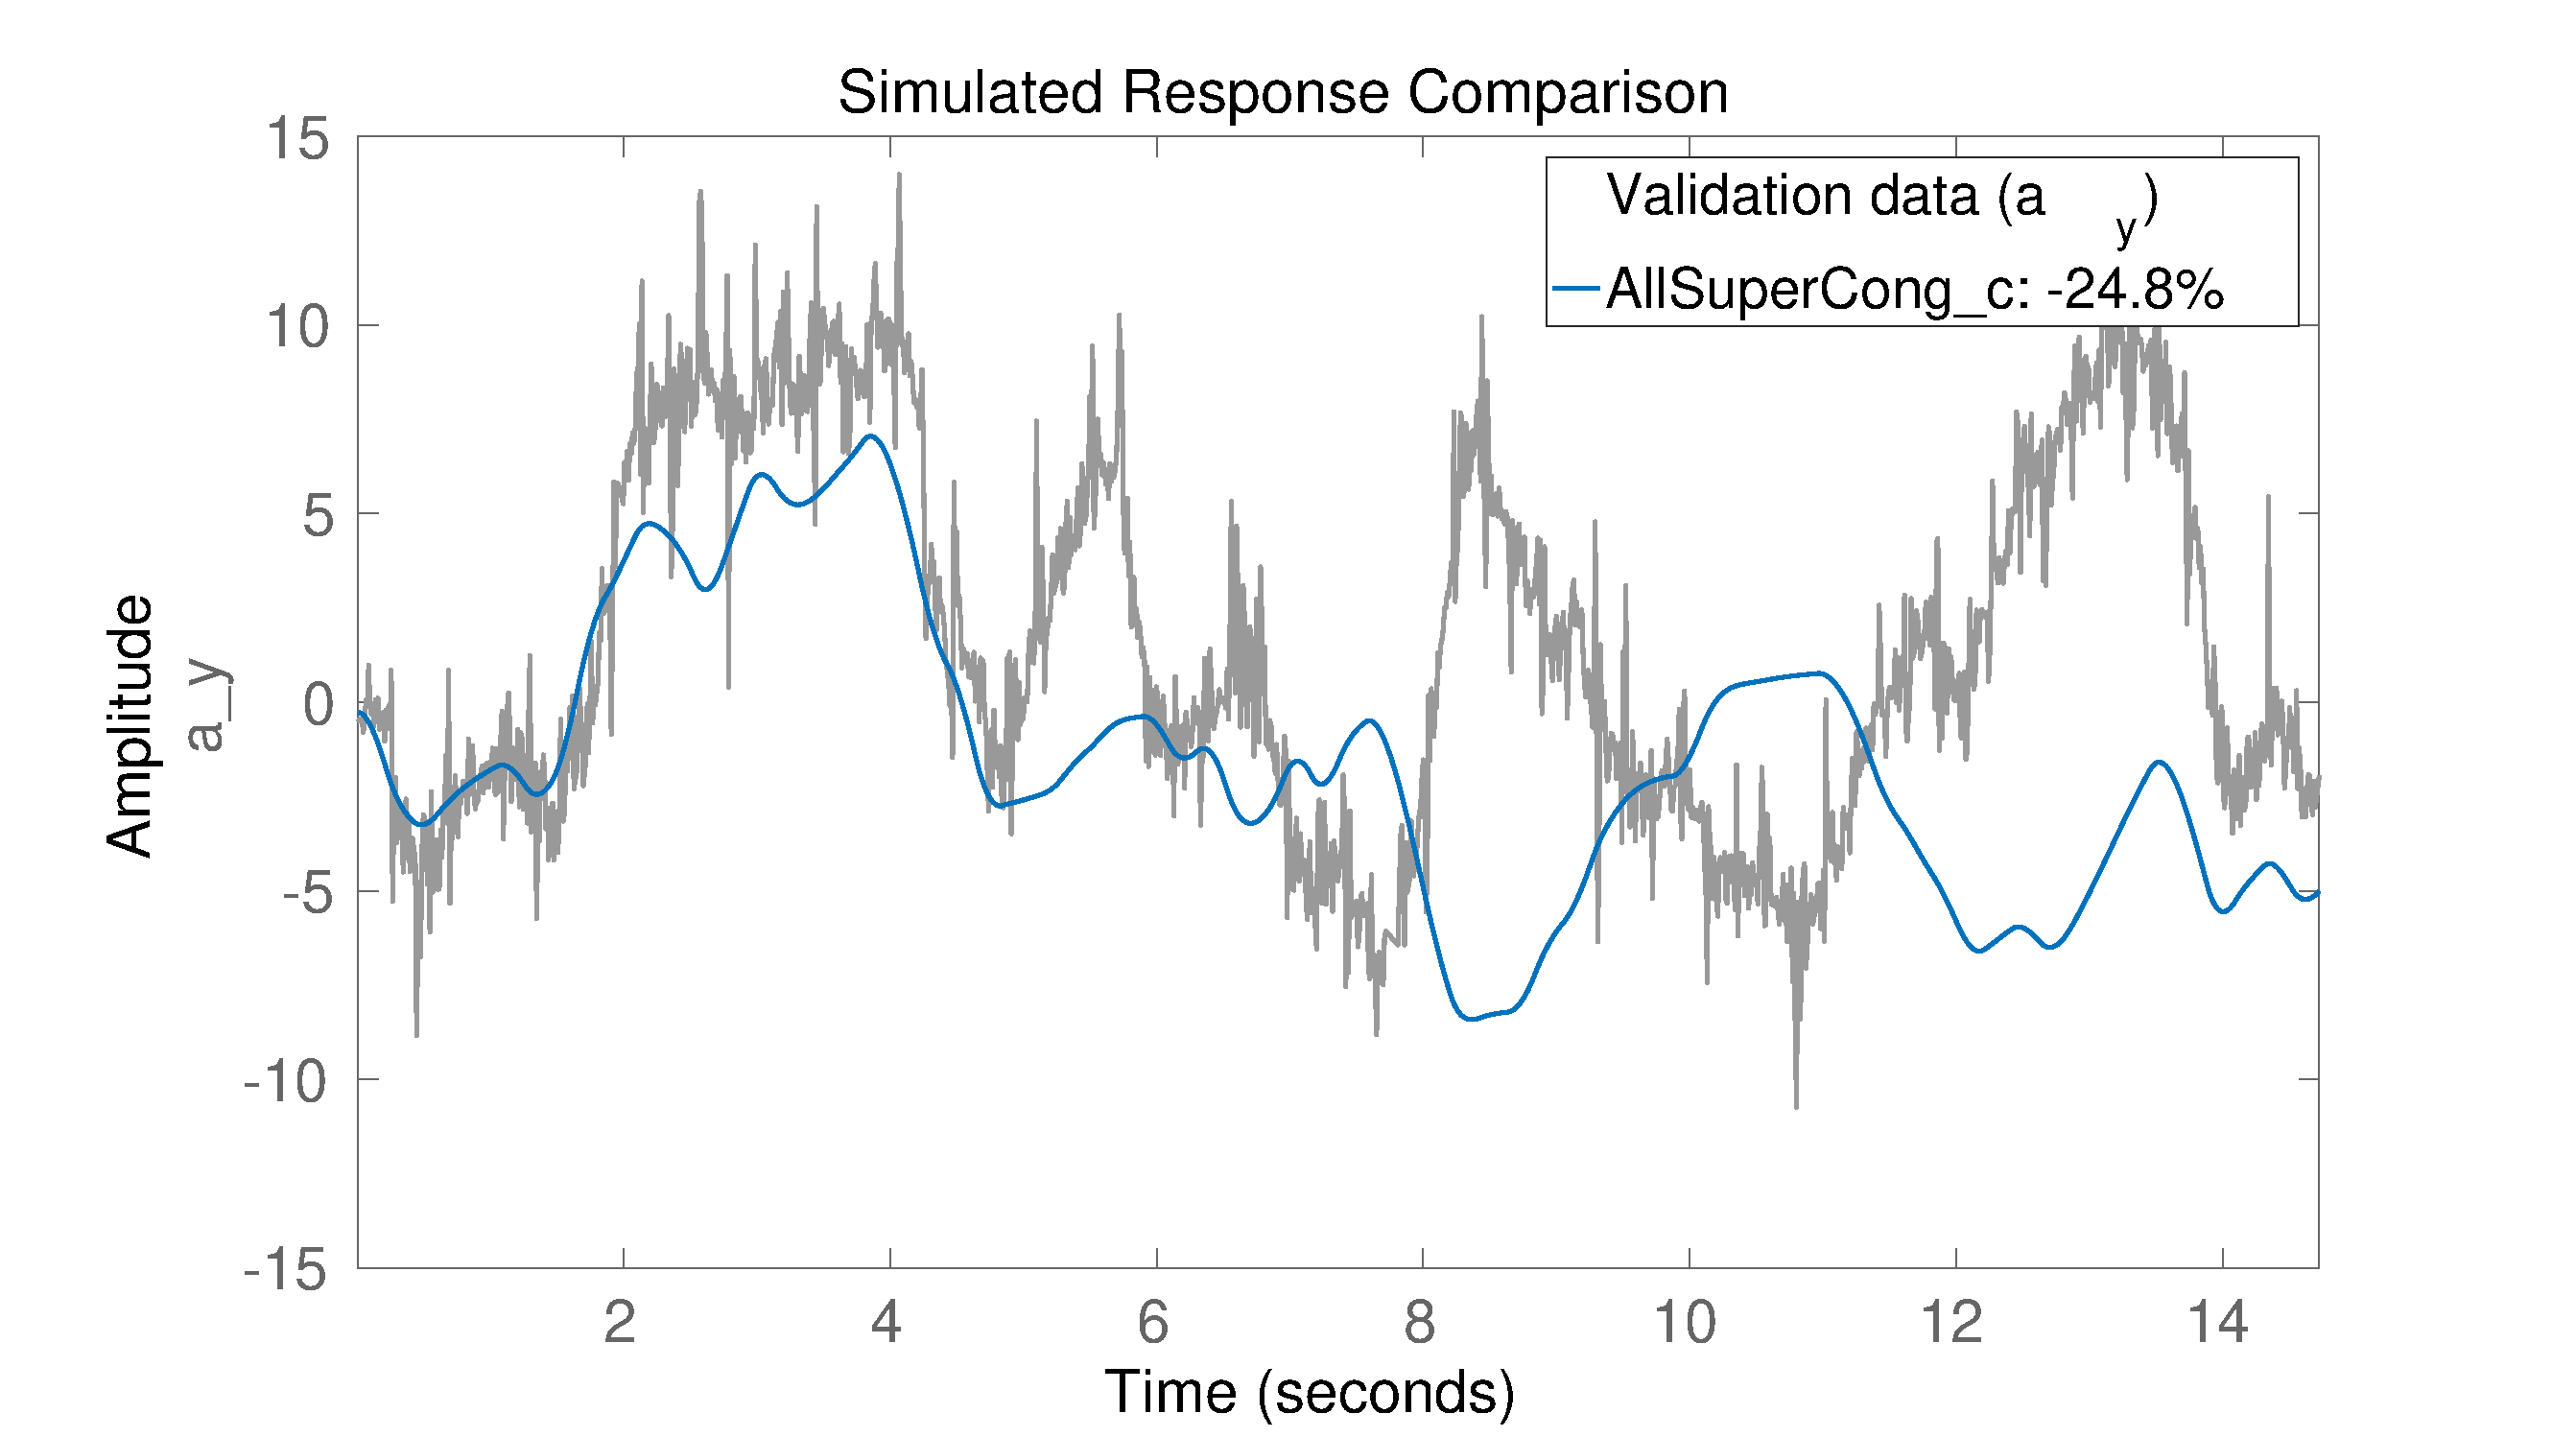
\includegraphics[width=0.4\textwidth]{linAccComparey}}
    \qquad
  \subfloat[][\label{fig:linAccComparez}Comparison of linear acceleration in the \abbrROV's z-axis between validation data and the simulated model.]{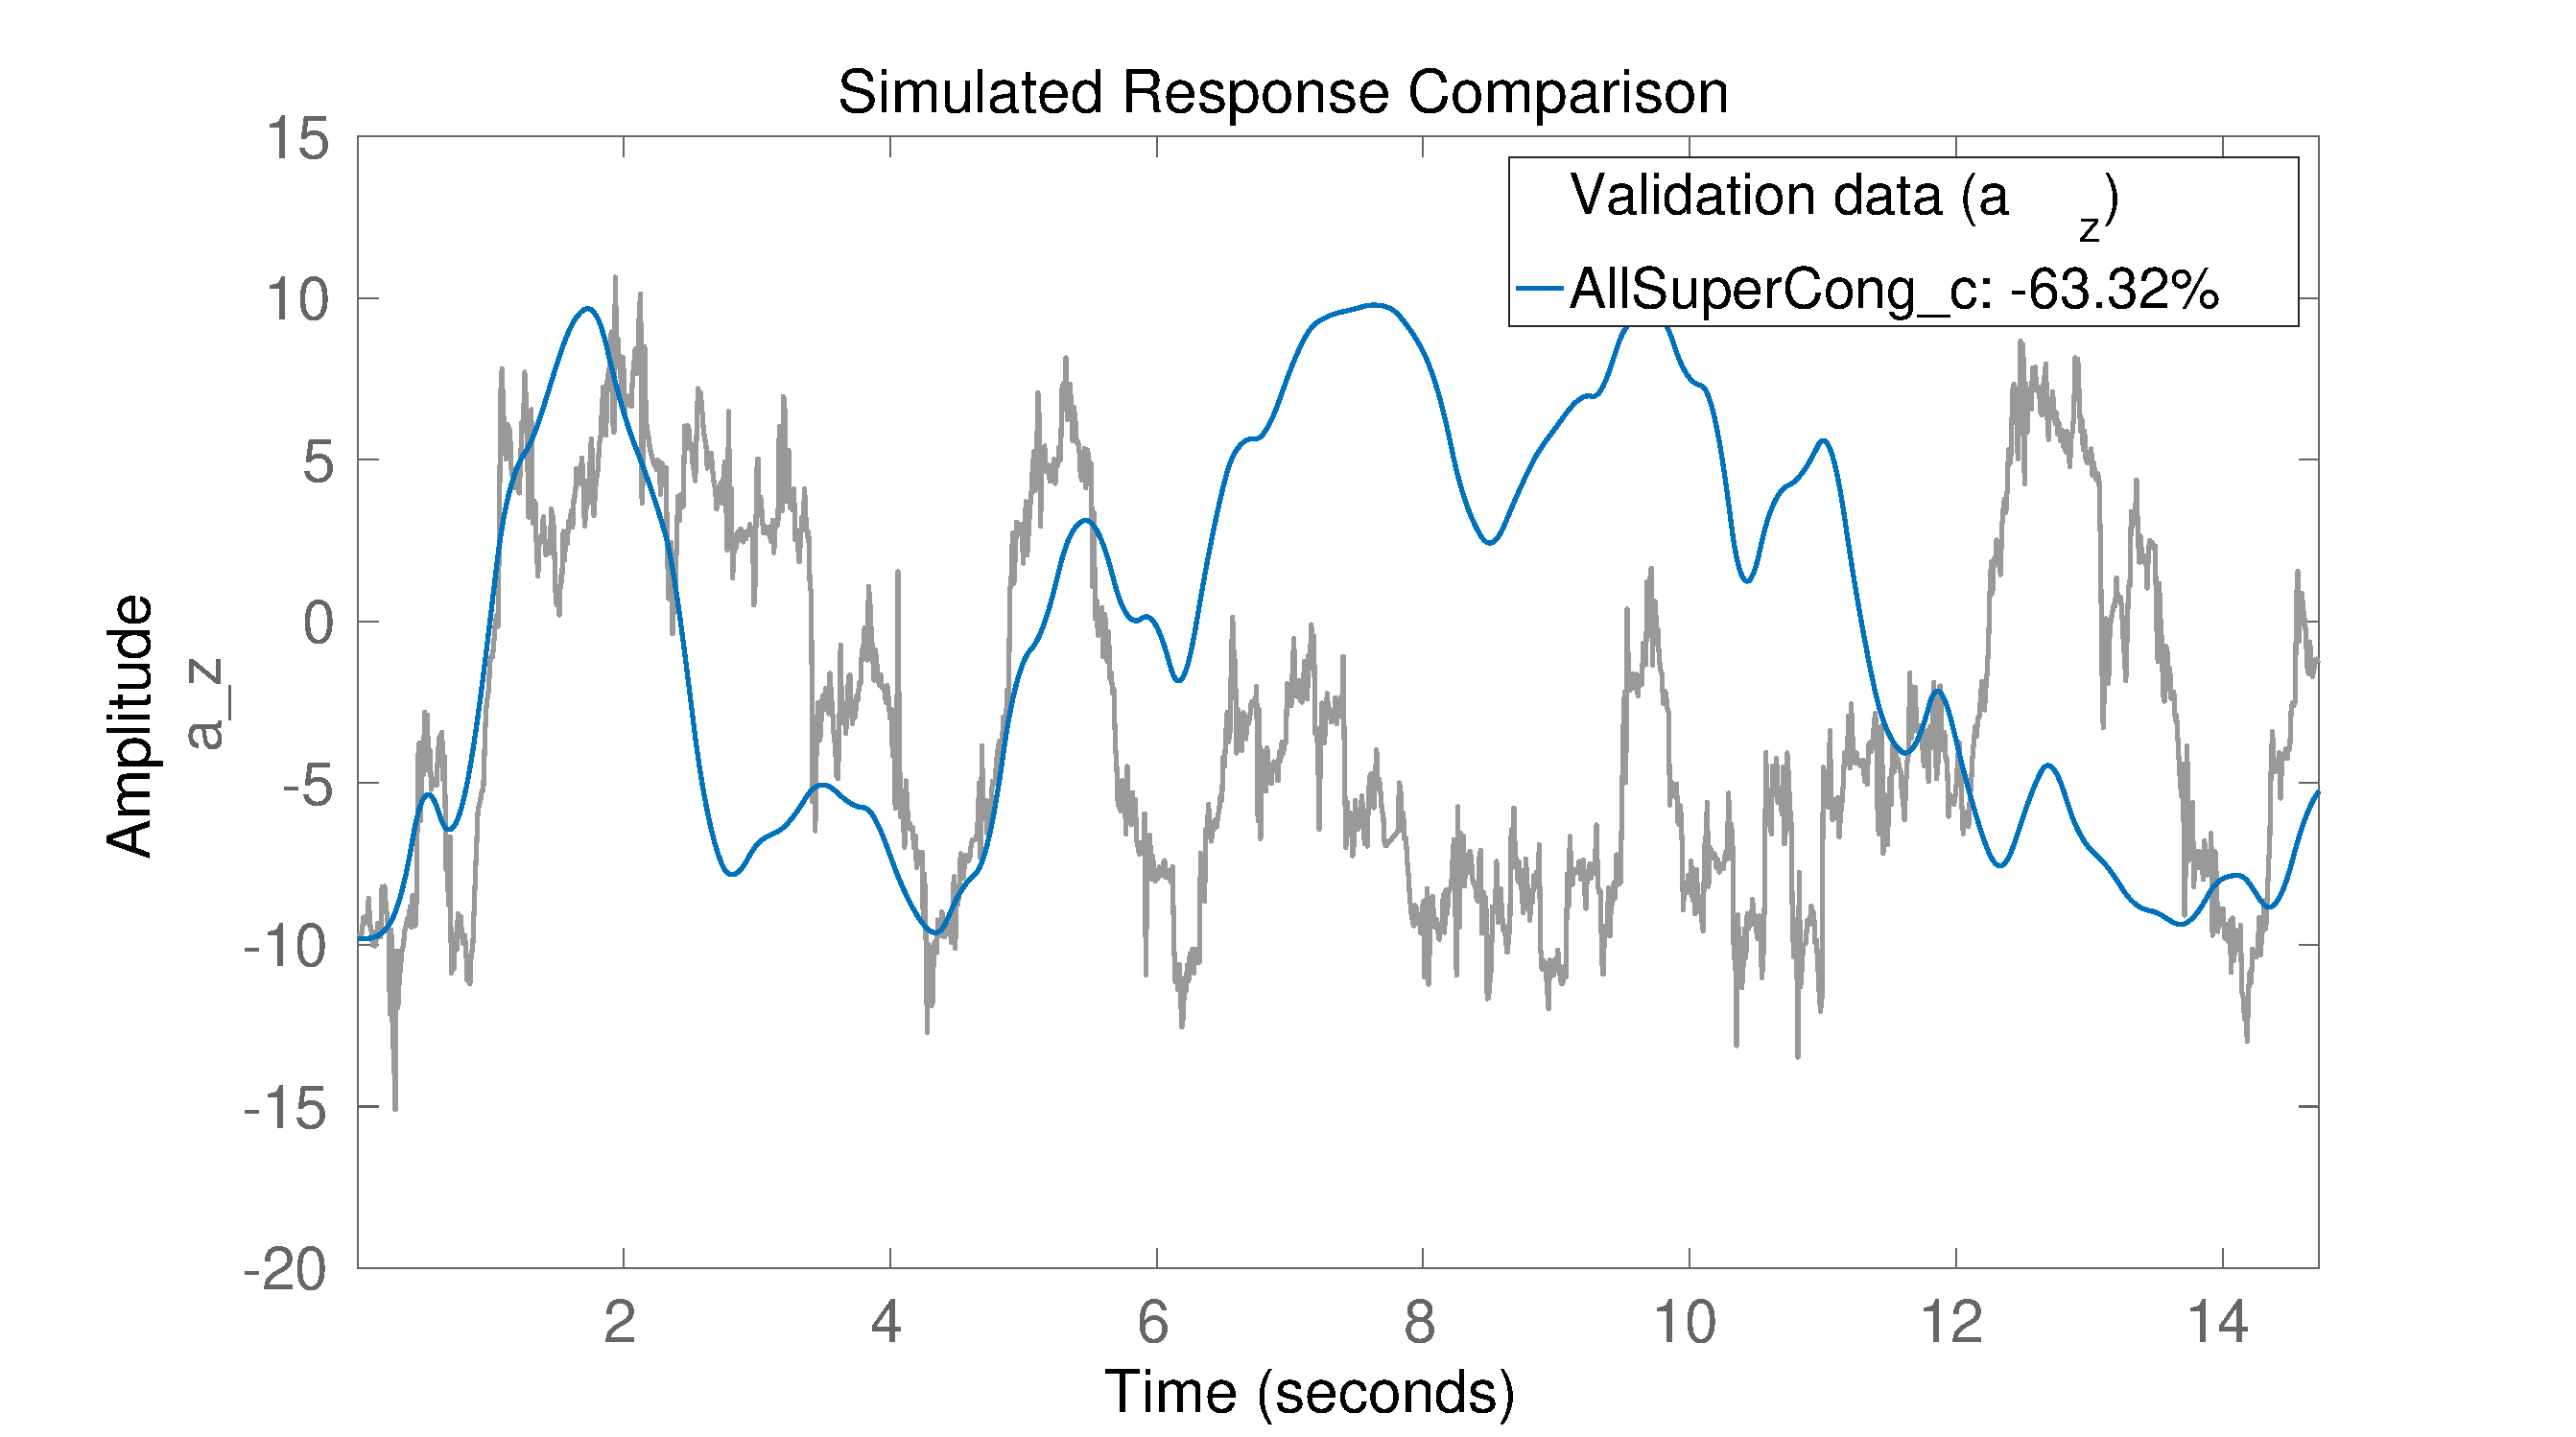
\includegraphics[width=0.4\textwidth]{linAccComparez}}
  \caption{\label{fig:angVelCompare}%
    Comparison of validation data (grey) against the simulated response from the model(blue). The fit for the model in each state is stated in each plot.}
\end{figure}
The fit of the model compared to validation data can be seen in \Figureref{fig:angVelCompare}. For estimating the parameters the initial states had to be well estimated. If the initial states of the model did not correspond well to the true initial states the parameters did not converge to the true values. This can be seen in \Figureref{fig:angVelSim} were estimation of the parameters was done on simulated data. The data was simulated with the same parameter values as the estimation was initlised with. A Kalman smoother as described in \citet{Wallin} has been used for initial state estimation. In the initial state estimation the magnetometer was used to reduce the uncertainty of the initial quaternions.
\begin{figure}[tbp]
  \centering
  \subfloat[][\label{fig:angVelSimp}Comparison of simulated angular velocity around the \abbrROV's x-axis with simulated validation data.]{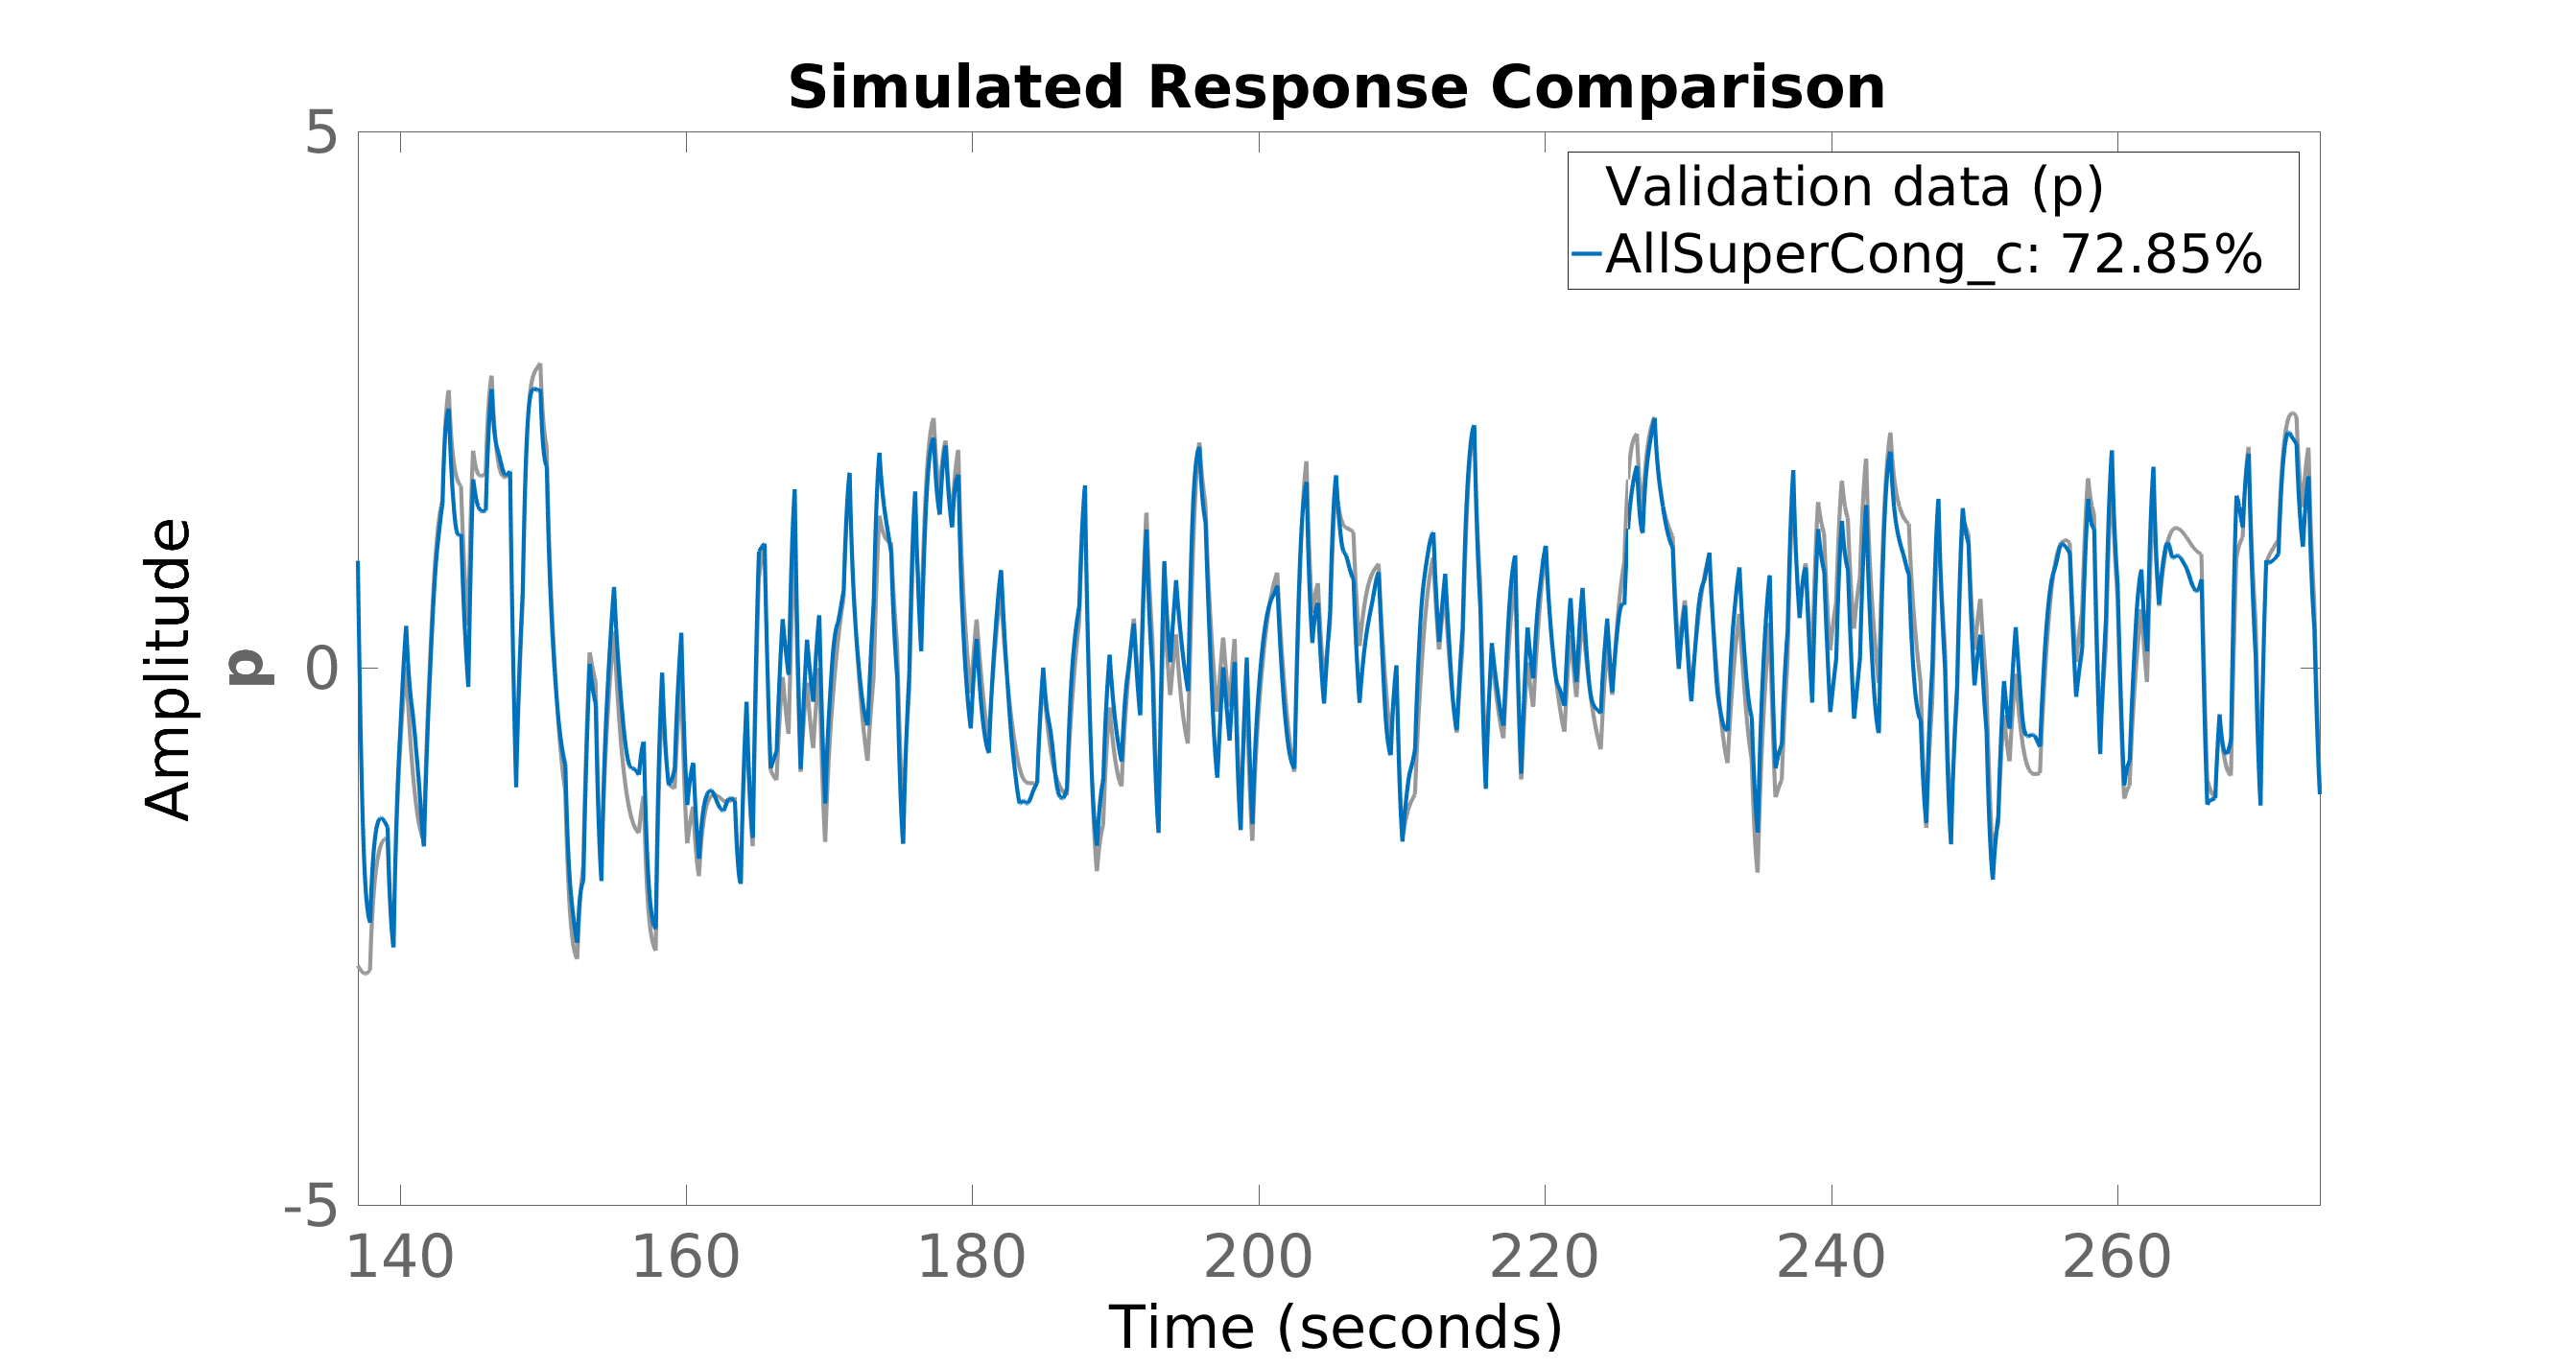
\includegraphics[width=0.4\textwidth]{angVelSimp}}
  \qquad
  \subfloat[][\label{fig:angVelSimq}Comparison of simulated angular velocity around the \abbrROV's y-axis with simulated validation data.]{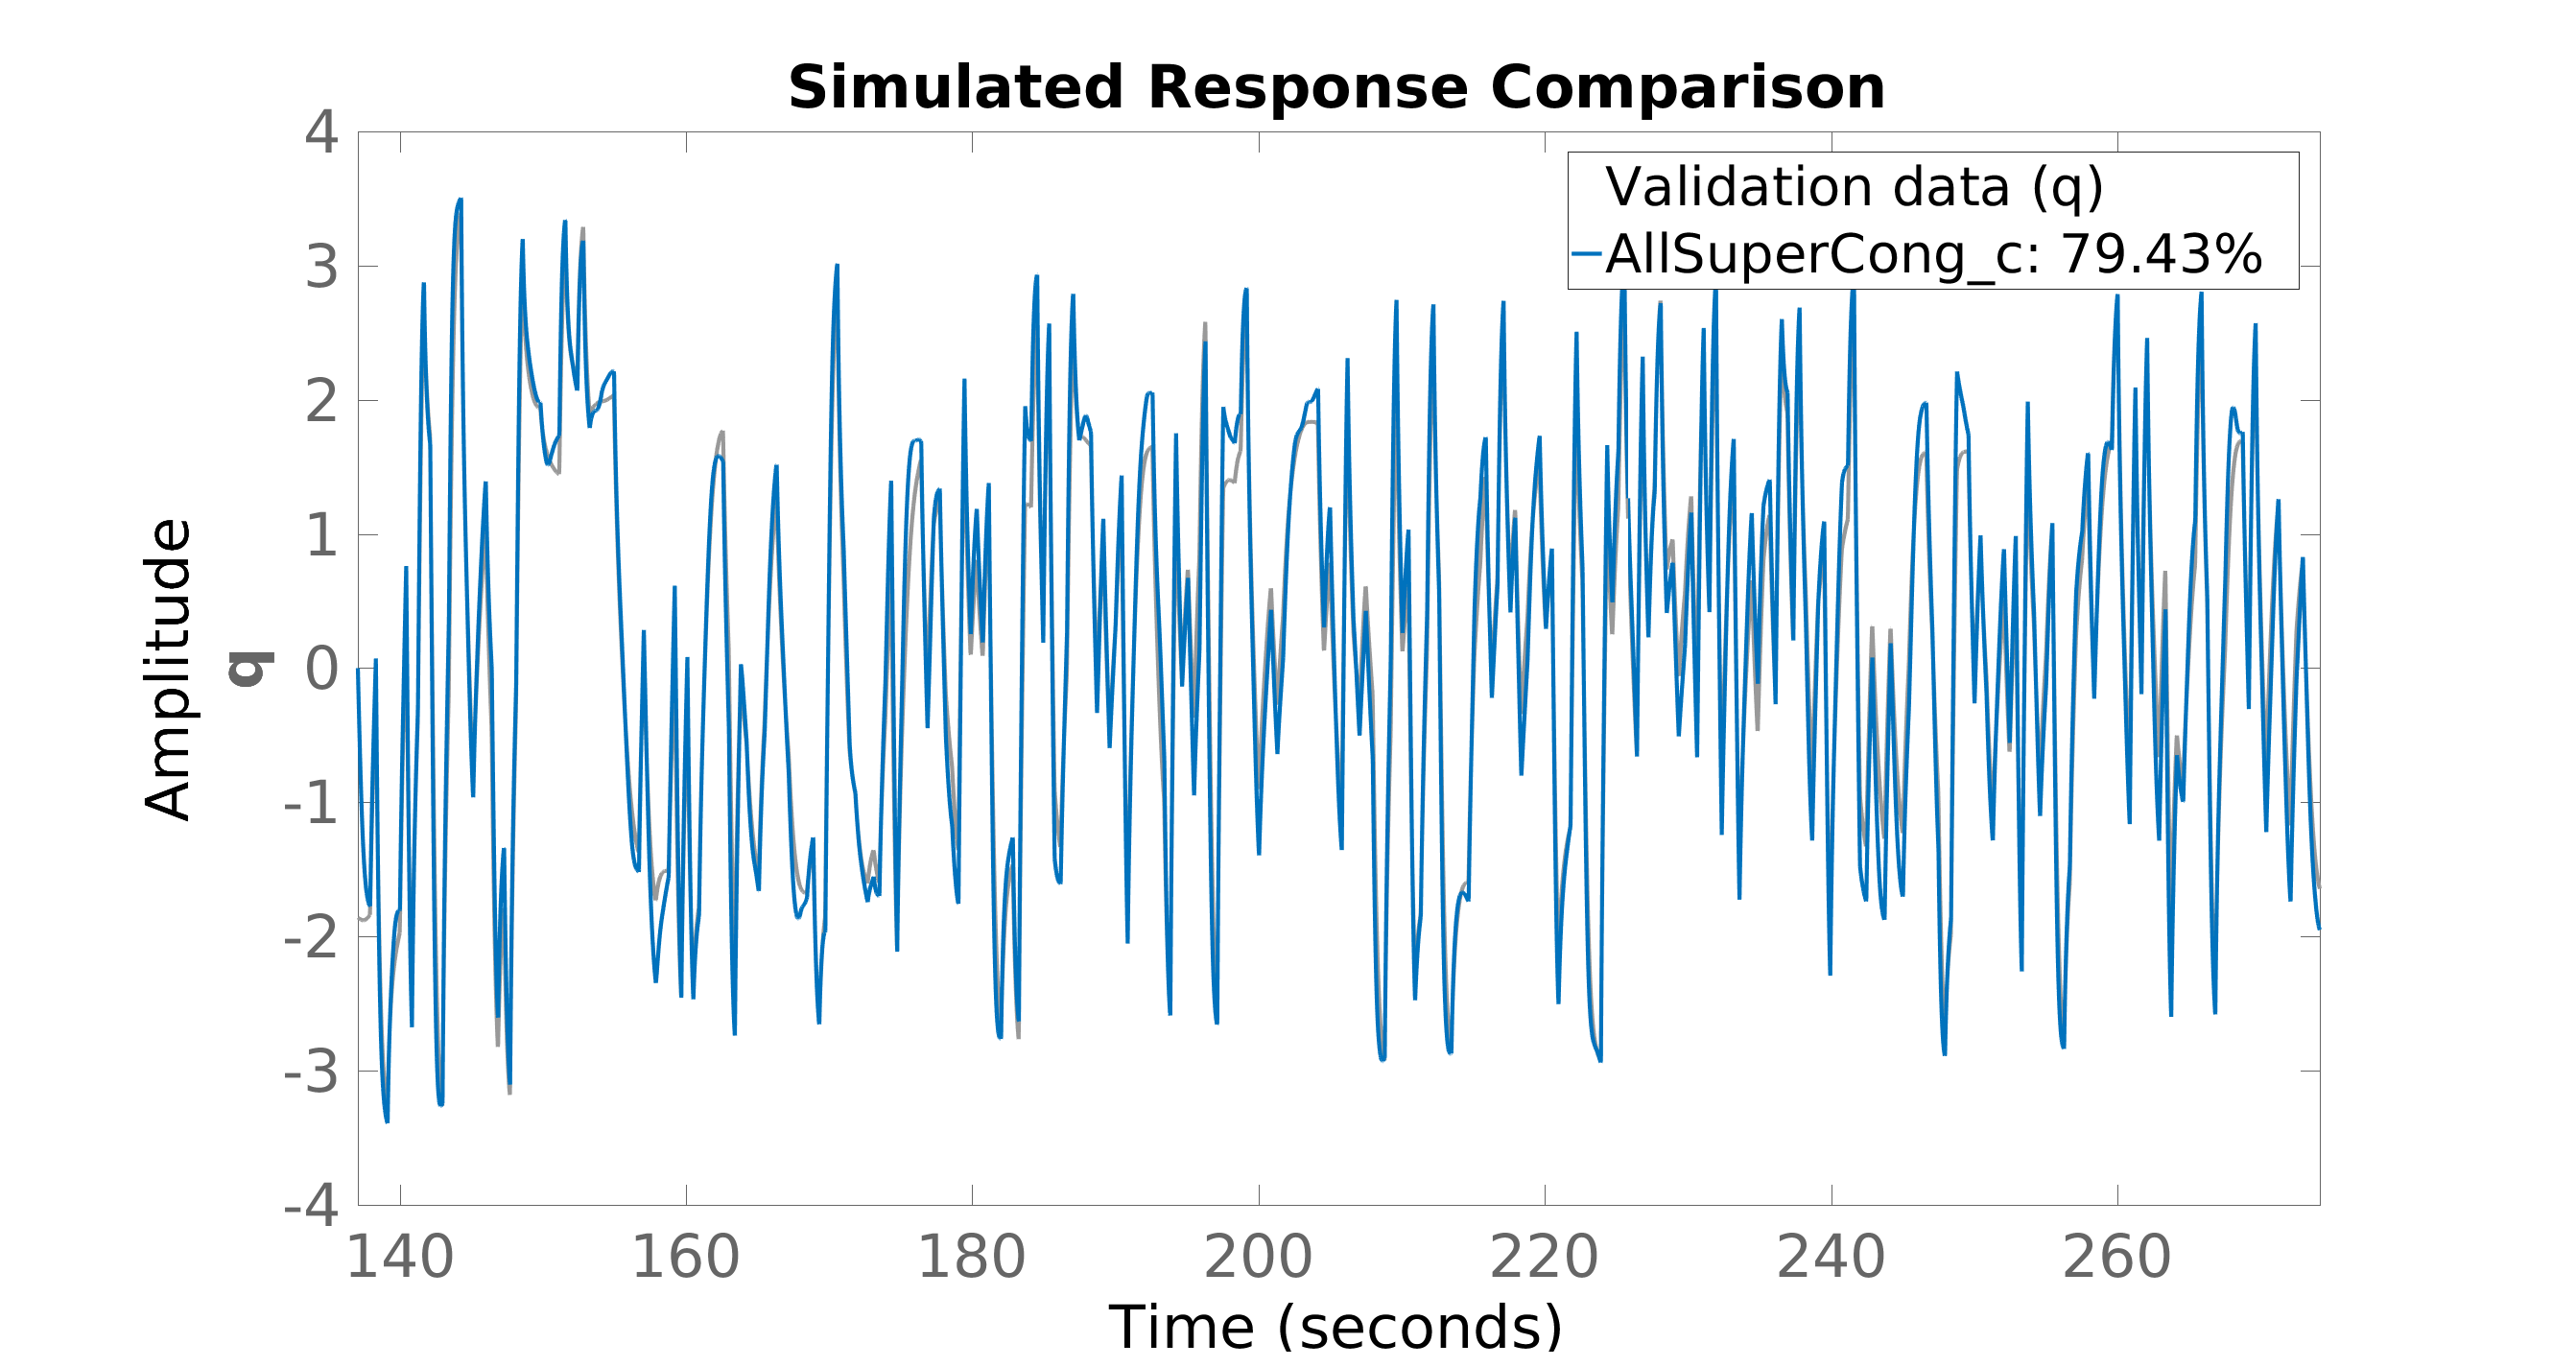
\includegraphics[width=0.4\textwidth]{angVelSimq}}
  \qquad
  \subfloat[][\label{fig:angVelSimr}Comparison of simulated angular velocity around the \abbrROV's z-axis with simulated validation data.]{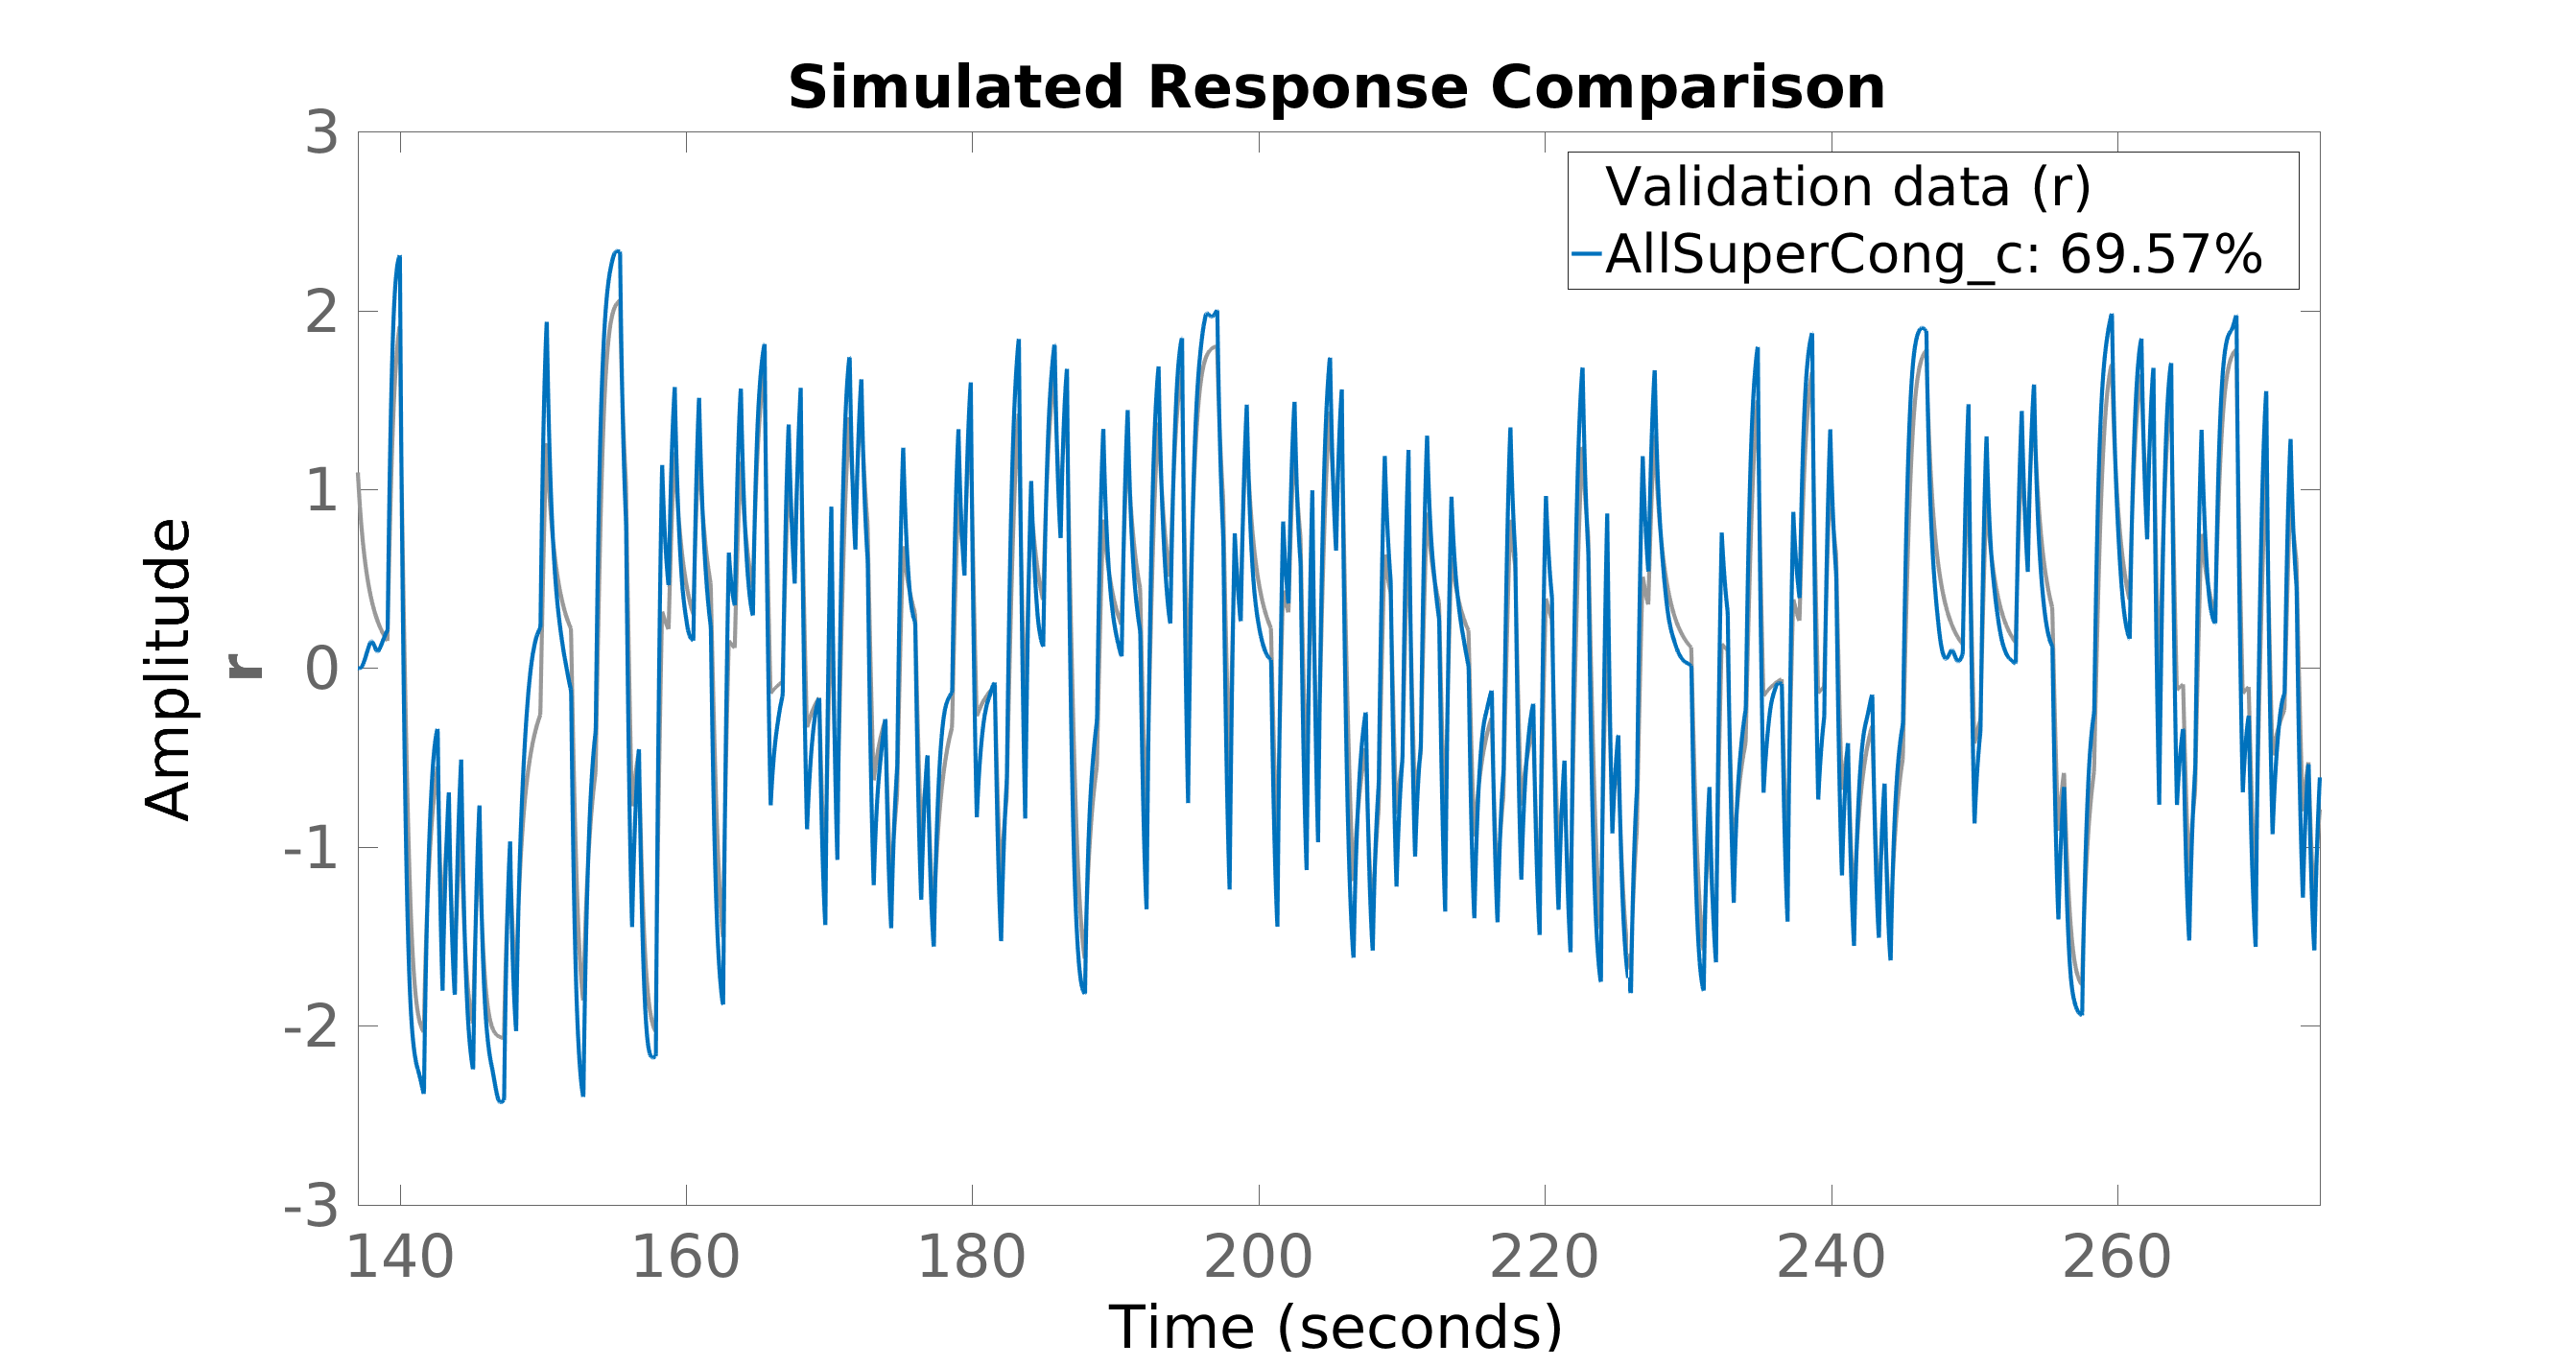
\includegraphics[width=0.4\textwidth]{angVelSimr}}
    \qquad
  \subfloat[][\label{fig:linAccSimx}Comparison of simulated linear acceleration in the \abbrROV's x-axis with simulated validation data.]{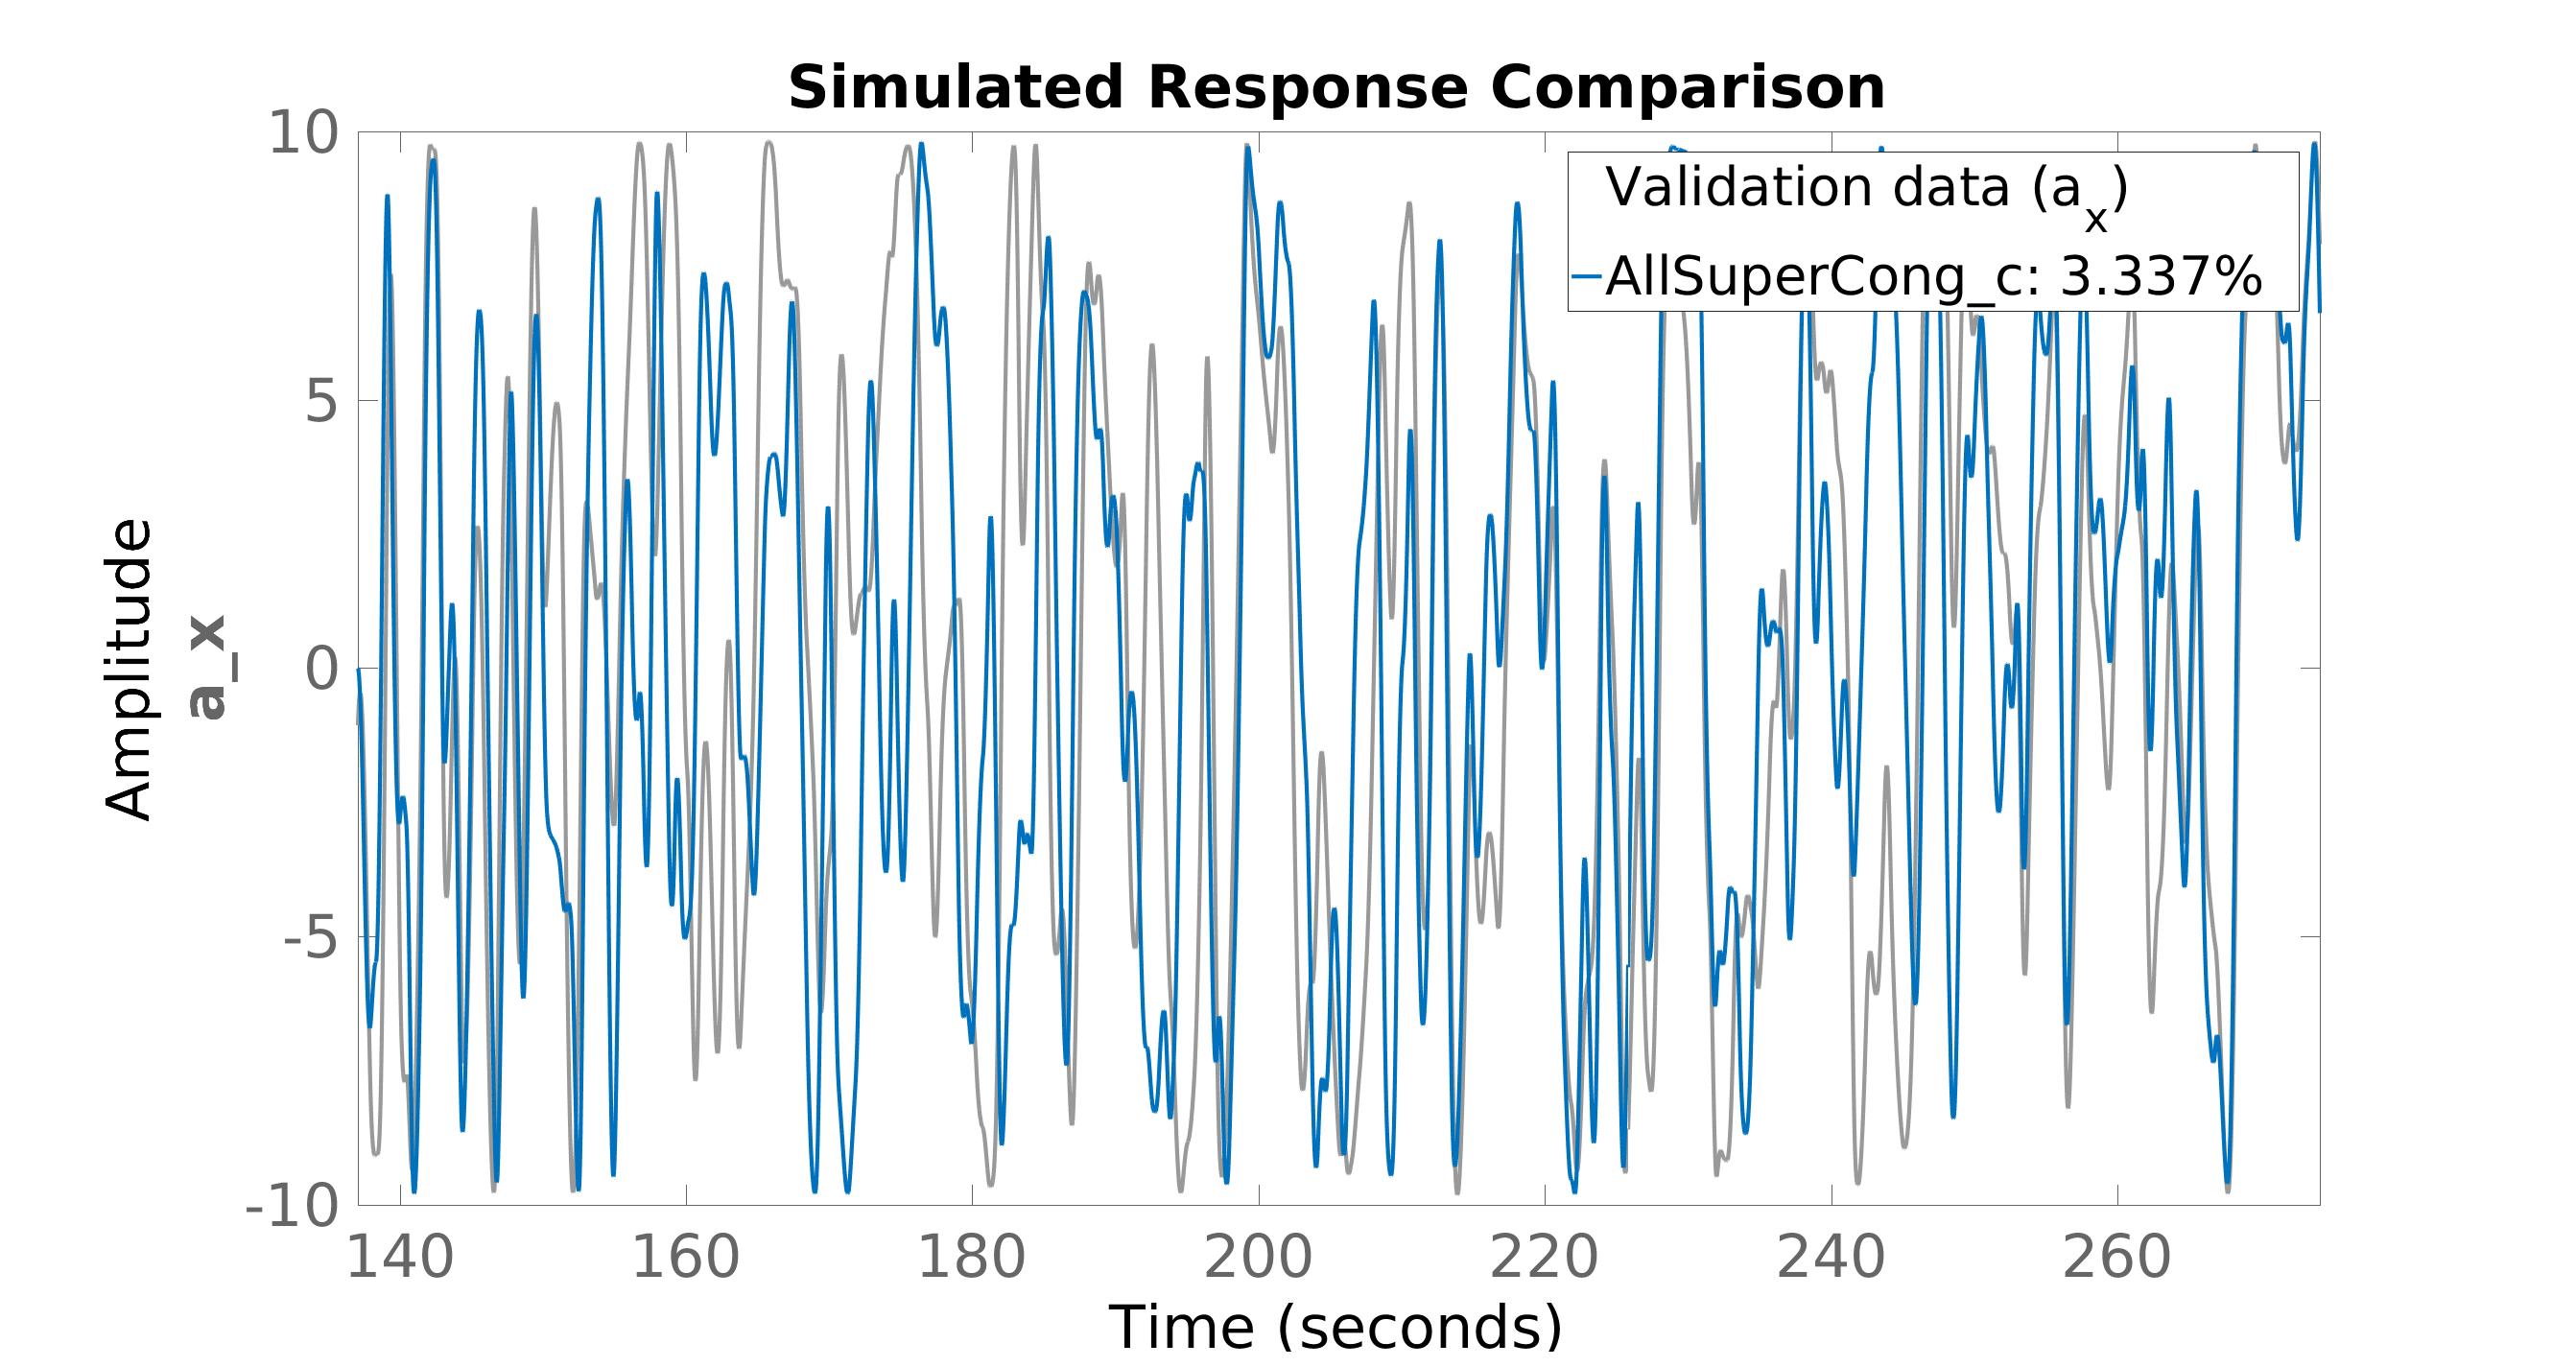
\includegraphics[width=0.4\textwidth]{linAccSimx}}
    \qquad
  \subfloat[][\label{fig:linAccSimy}Comparison of simulated linear acceleration in the \abbrROV's y-axis with simulated validation data.]{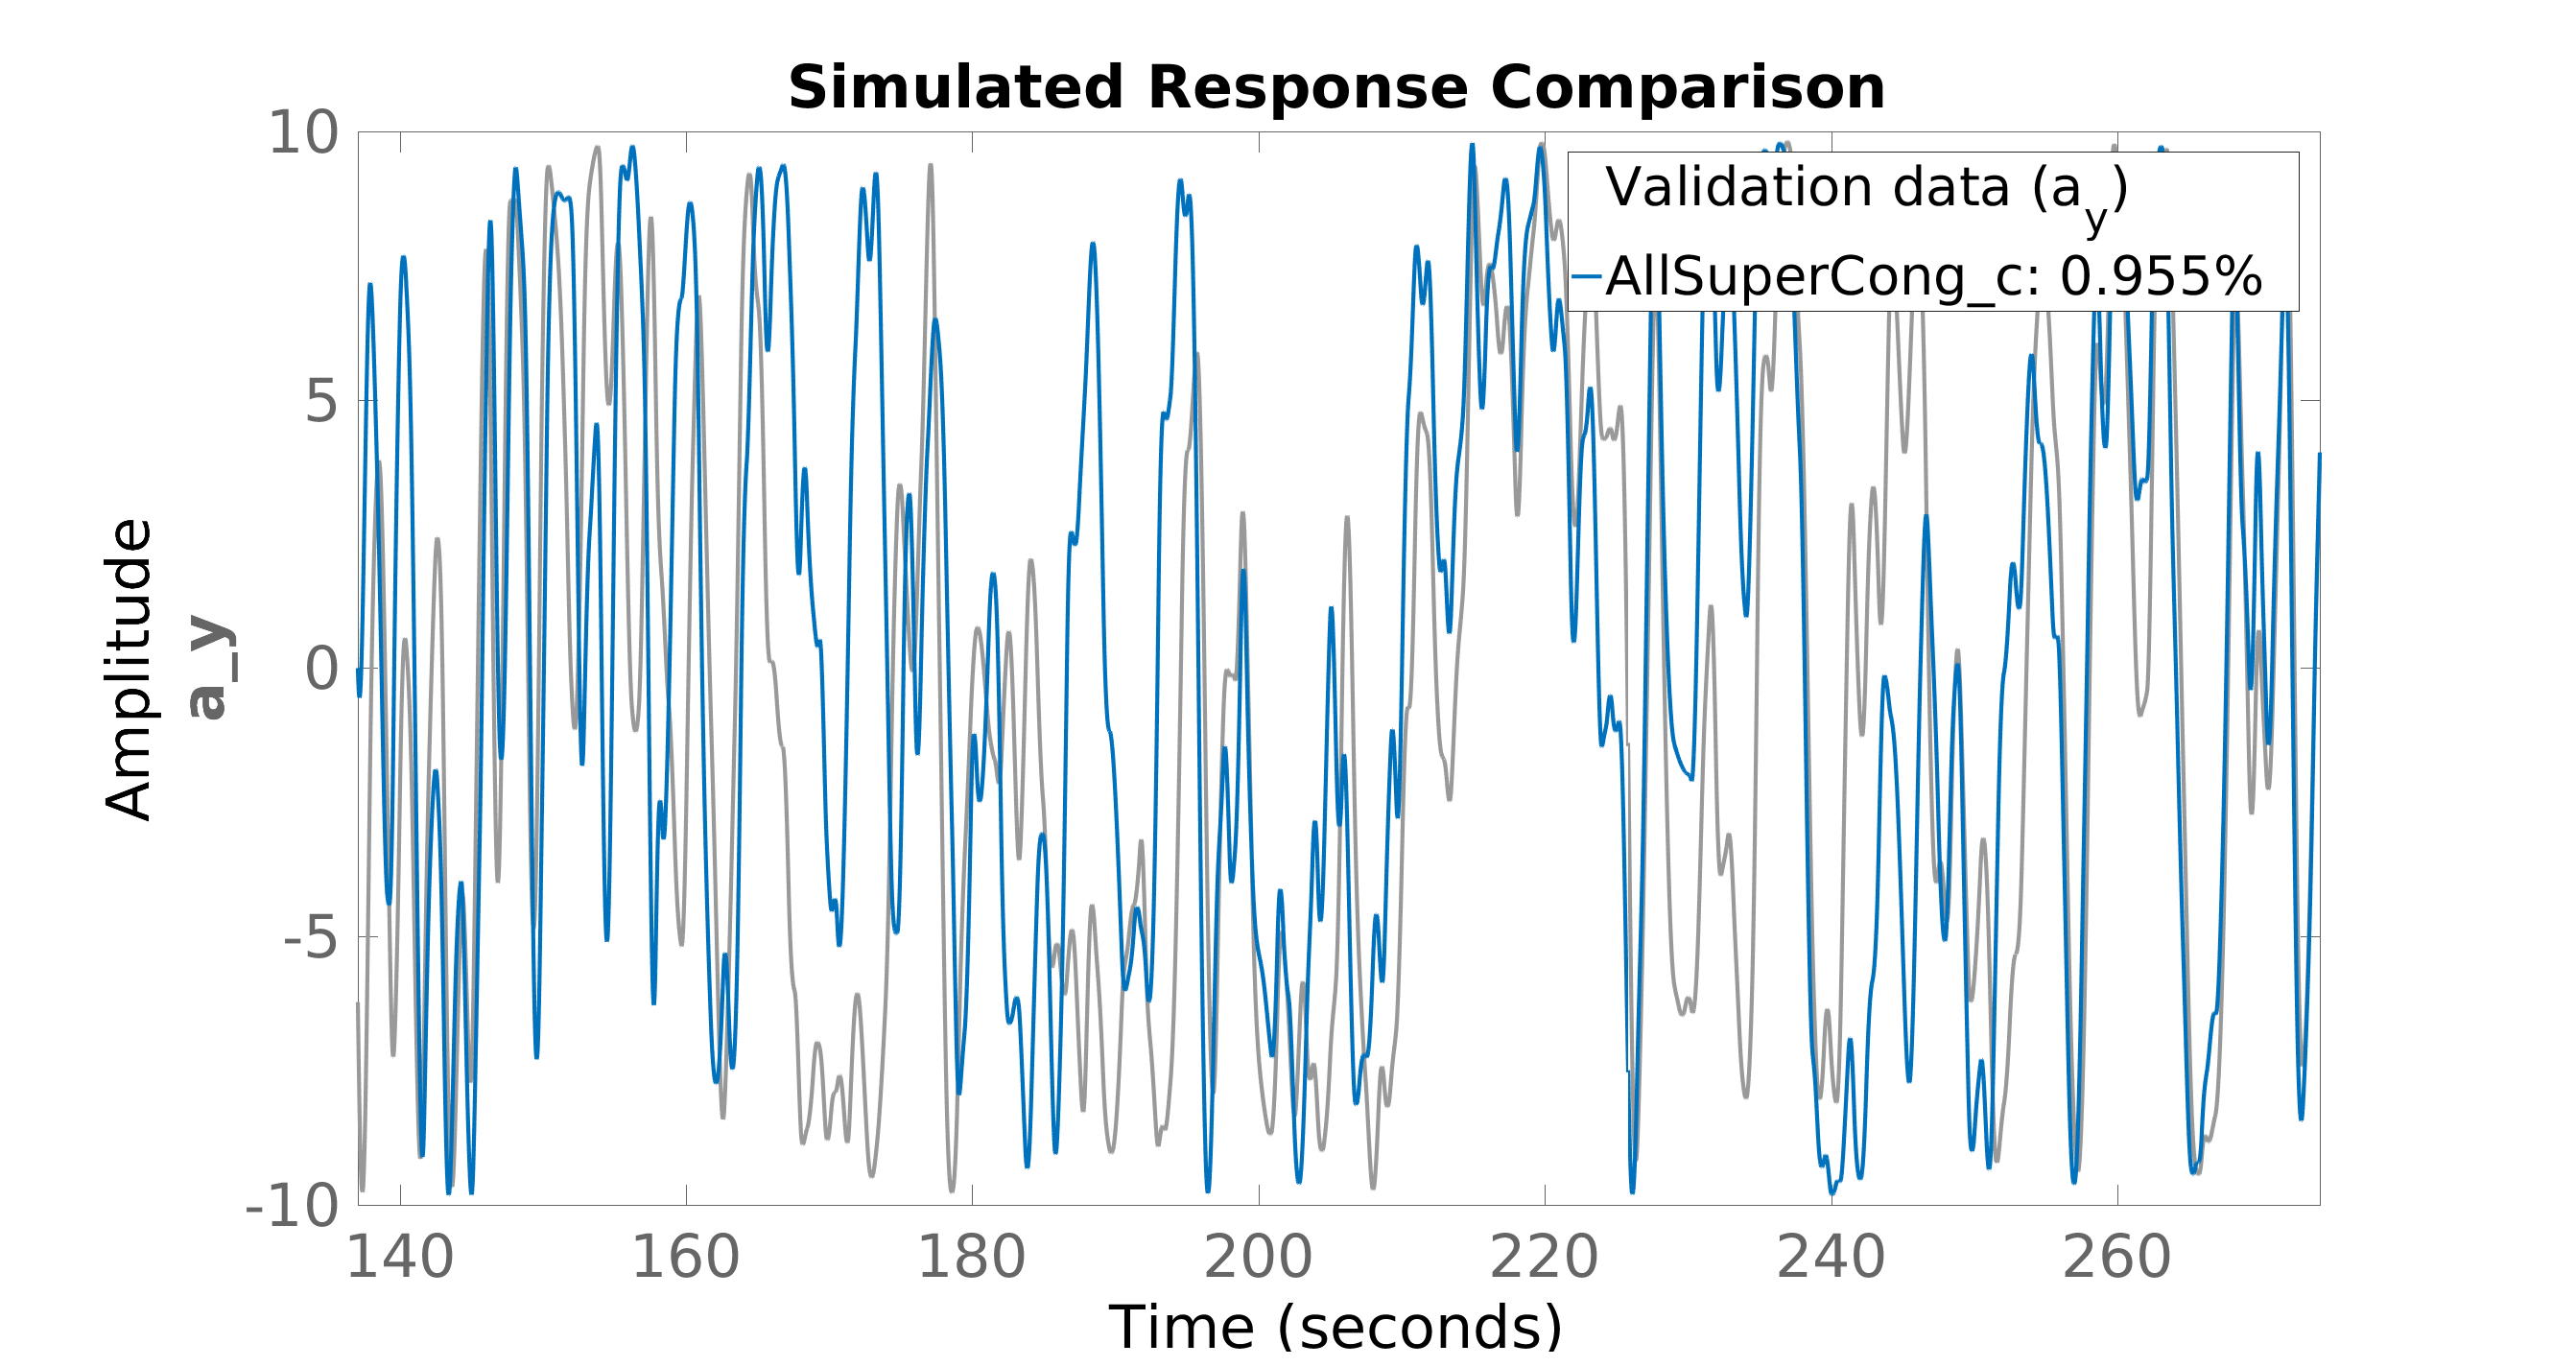
\includegraphics[width=0.4\textwidth]{linAccSimy}}
    \qquad
  \subfloat[][\label{fig:linAccSimz}Comparison of simulated linear acceleration in the \abbrROV's z-axis with simulated validation data.]{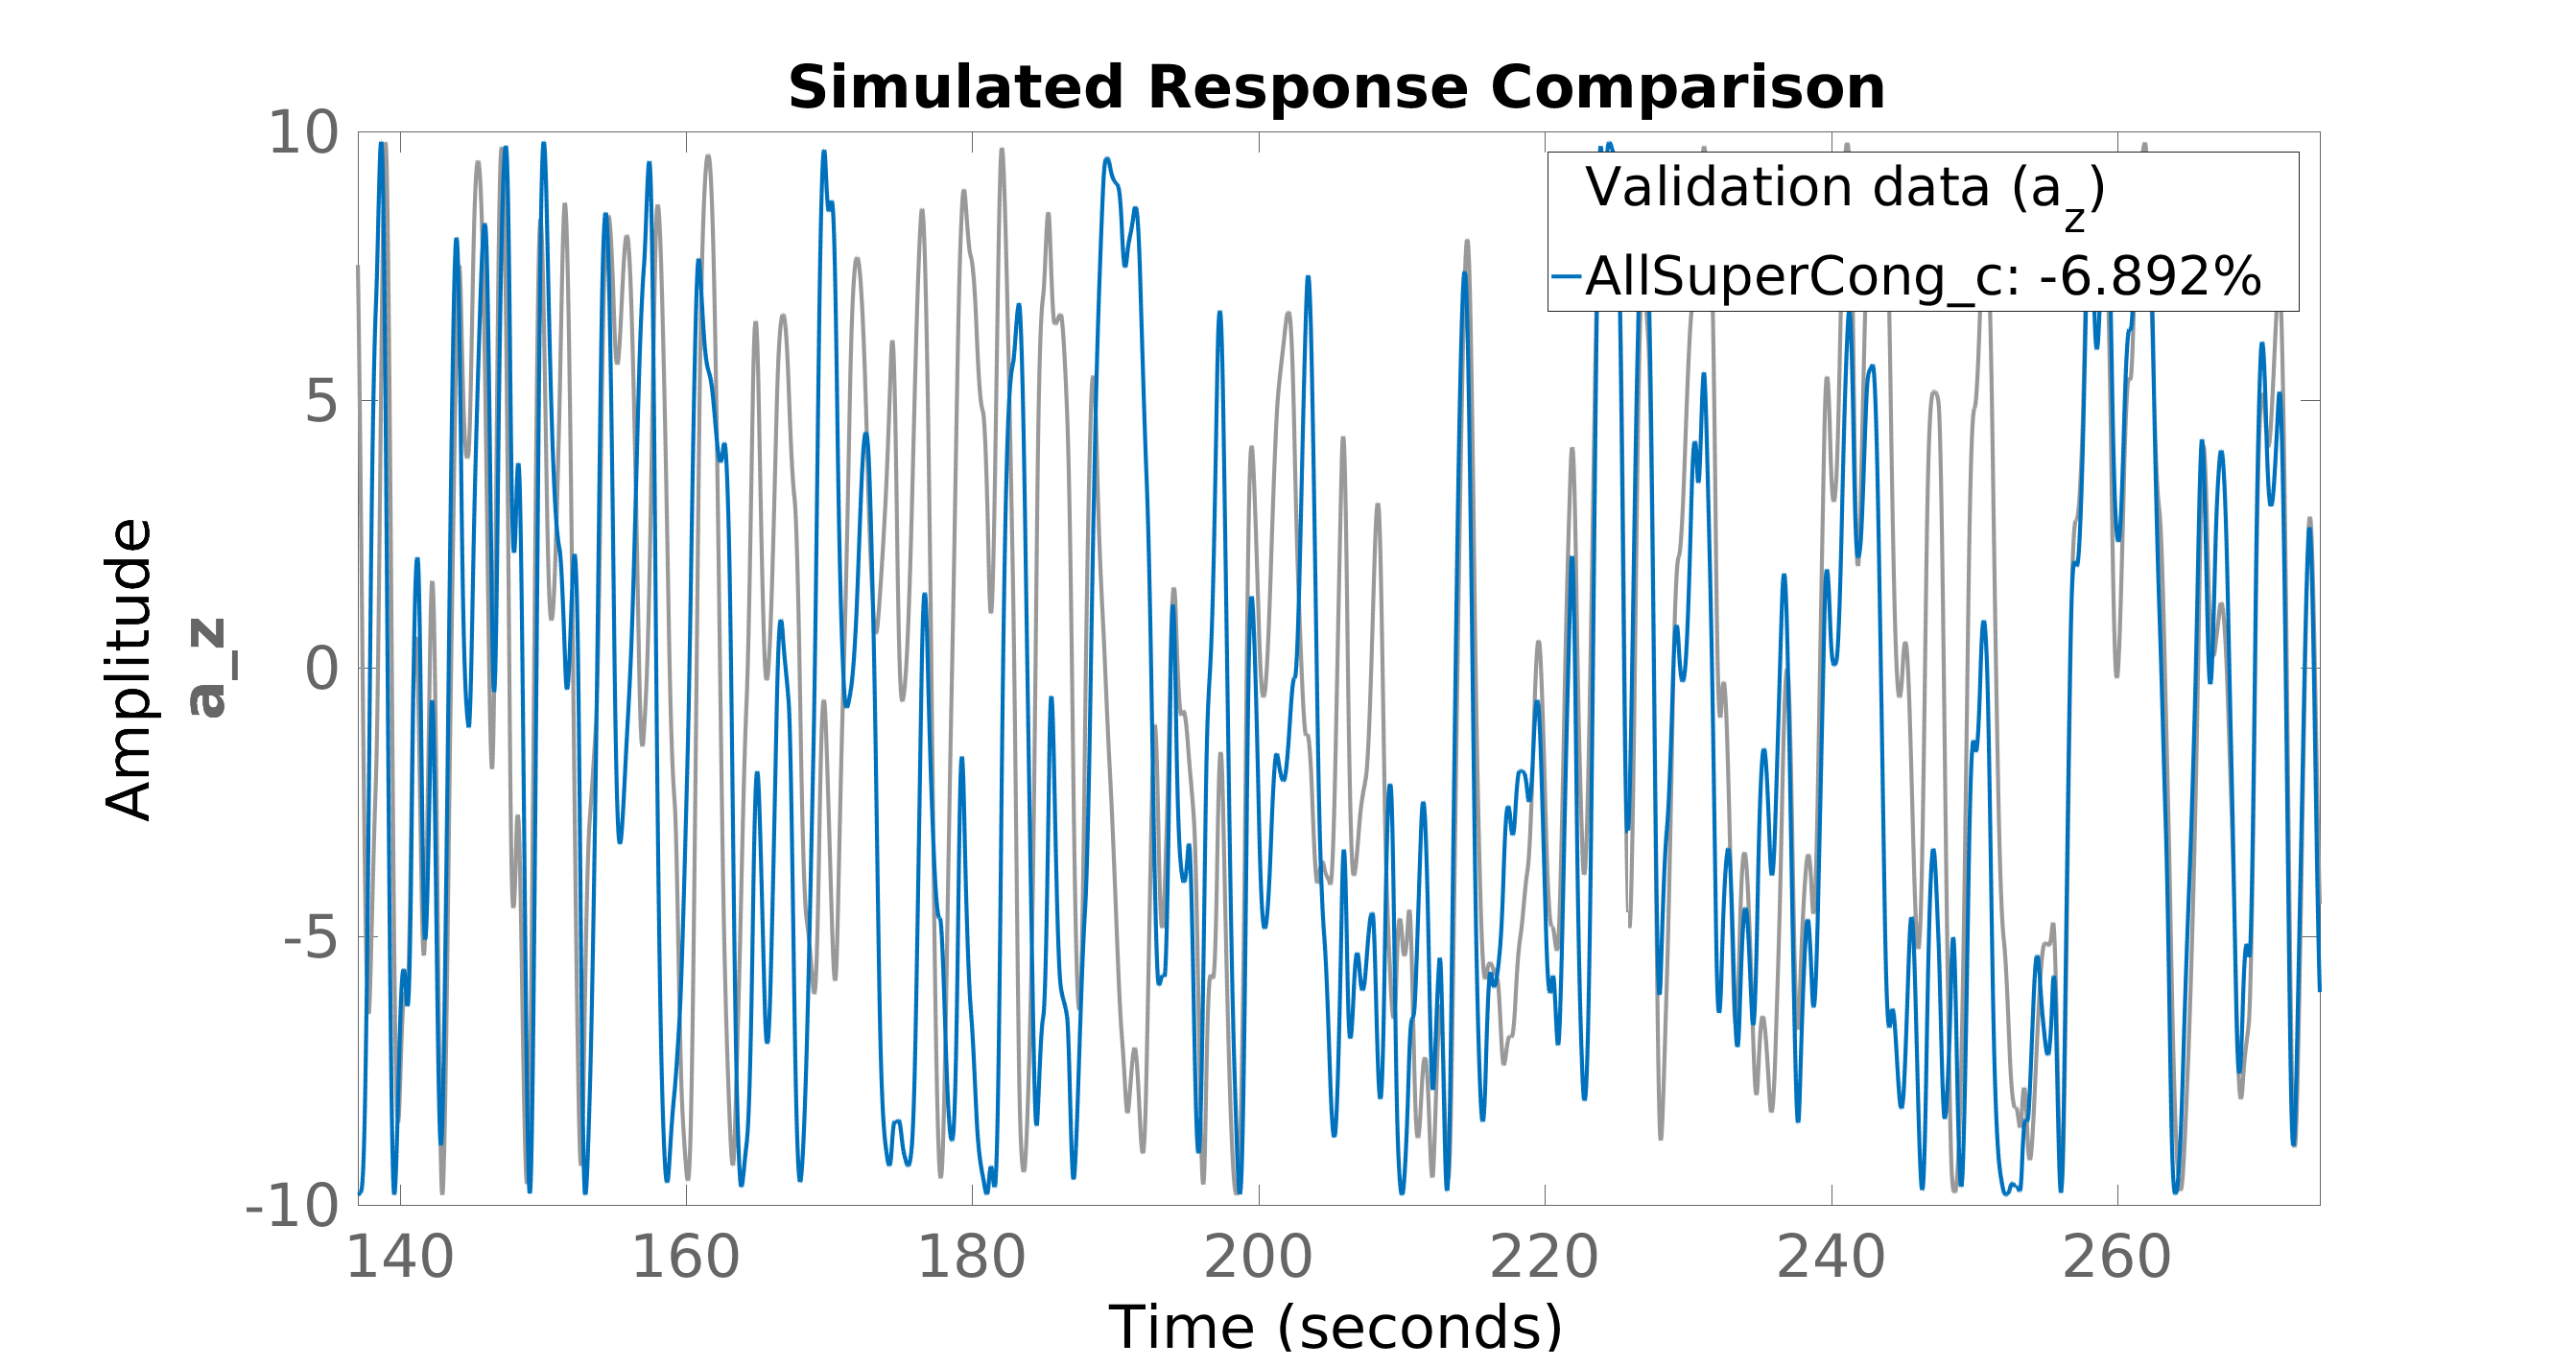
\includegraphics[width=0.4\textwidth]{linAccSimz}}
  \caption{\label{fig:angVelSim}%
    Comparison between simulated validation data (grey) and the simulated response from the model(blue). The fit for the model in each state is stated in each plot. The validation data has been generated from the initial parameters in the parameter estimation. The initial states of the model has been altered and thus the parameter estimation can not find the correct parameters.}
\end{figure}

To handle noisy signals an error threshold was introduced. An error threshold means that after a breakpoint the cost function becomes linear instead of squared. This makes the parameter estimation less sensitive to outliers. To reduce the impact of the noise even further the used weight matrix in the cost function was the inverse of the estimated noise covariance. 

%%%%%%%%%%%%%%%%%%%%%%%%%%%%%%%%%%%%%%%%%%%%%%%%%%%%%%%%%%%
\subsection{Extended Kalman filter estimation}\index{EKF@\abbrEKF!abbreviation}
A \abbrEKF was also used to estimate parameters of the \abbrROV. The reparametrised model from \Sectionref{sec:angLinEstim} was used to model $\etaVector$ and $\nuVector$. Measurement equations were taken from \Chapterref{cha:sensor_fusion}. Each model parameter was modelled as a state using a constant position motion model. The entire motion model used in the filter was discretised using the Euler forward discretisation method. The complete discrete model is
\begin{equation}
\label{eq:motionModelKalman}
\begin{pmatrix}
\etaVector_{k+1}\\ 
\nuVector_{k+1}\\
\boldsymbol{b}_{k+1}\\
\boldsymbol{\theta}_{k+1}
\end{pmatrix} = 
\begin{pmatrix}
\etaVector_k + T_s \boldsymbol{T}(\etaVector_k)\nuVector_k\\
\nuVector_k + T_s f(\etaVector_k,\nuVector_k,\boldsymbol{\theta}_k)\\
\boldsymbol{b}_k\\
\boldsymbol{\theta}_k
\end{pmatrix}
+ \begin{pmatrix}
\boldsymbol{v}_{\etaVector}\\
\boldsymbol{v}_{\nuVector}\\
\boldsymbol{v}_{\boldsymbol{b}}\\
\boldsymbol{v}_{\boldsymbol{\theta}}
\end{pmatrix}
\end{equation}
Here $\boldsymbol{\theta}$ is a vector containing the reparametrised parameters that were estimated. $f(\etaVector,\nuVector,\boldsymbol{\theta})$ is the model defined in \Chapterref{cha:modelling} using quaternions and with reparameterised parameters defined in \Sectionref{sec:estimation_angular}. $\boldsymbol{b}$ is a vector containing the biases of the gyroscope. $\boldsymbol{v}$ is model noise and is assumed to enter each term directly, this resulted in a diagonal $\boldsymbol{Q}$-matrix when implementing the model in the \abbrEKF. $\boldsymbol{T}(\etaVector)$ is a angular velocity transformation matrix using the quaternion form of $\etaVector$ and is defined in \Chapterref{cha:modelling}.

To increase the performance of the filter a method for outlier detection and rejection was implemented.
The outlier rejection method is based on the assumption that the normalised innovation $\boldsymbol{\epsilon}^T \boldsymbol{S}^{-1} \boldsymbol{\epsilon}$ should be $\chi_{n}^{2}$ distributed. Here $n$ is the number of measurements. To check the validity of a single measurement the previous asumption gives that $\epsilon_i^{2}/S_{i,i} \sim \chi_{1}^{2}$ \citep{sensorfusion}. This is used in the \abbrEKF using the following algorithm:
\begin{algorithm}[H]
\label{alg:outlier}
\caption{The outlier rejection algorithm used during the measurement update step of the parameter estimation \abbrEKF.}
\textbf{1.} Calculate $\boldsymbol{S}=\boldsymbol{H} \boldsymbol{P} \boldsymbol{H}^T + \boldsymbol{R}$ and the innovation $\epsilon$.
\\
\textbf{2.} For each row $i$ in $\boldsymbol{\epsilon}$ do the comparison
\begin{equation}
\epsilon_{i}^{2} > \sigma_i S_{i,i}
\end{equation}
If the expression holds true remove the $i$:th row from $\boldsymbol{\epsilon}$ and the $i$:th row and column from $\boldsymbol{S}$ and $\boldsymbol{H}$.\\
\textbf{3.} Proceed with the Kalman algorithm using the cropped $\boldsymbol{H}$, $\boldsymbol{S}$ and $\boldsymbol{\epsilon}$.
\end{algorithm}
Here $\boldsymbol{\sigma}$ is a $n\times1$ dimensional design variable and $n$ is the number of measurements that are used in the \abbrEKF. A higher value of $\sigma_i$ decreases the sensitivity of the outlier rejection on the $i$:th measurement.

The filter was run on each collected dataset. The final values of $\hat{\boldsymbol{\theta}}$ from a dataset were used as initial values for $\hat{\boldsymbol{\theta}}$ when the filter was applied on the next dataset. The same was done for the covariance matrix $\boldsymbol{P}$. The final covariance from an earlier run was set as the initial covariance when the filter was applied on subsequent dataset. At completion the parameters were entered in a simulator which was feed with the control signals from the corresponding dataset. The simulated  output was then compared with the original data. The result from a typical estimation can be viewed in \Figureref{fig:KalmanCompare}.
\begin{figure}[tbp]
  \centering
  \subfloat[][\label{fig:KalmanCompareP}Comparison between a simulated model response and validation data in $p$.]{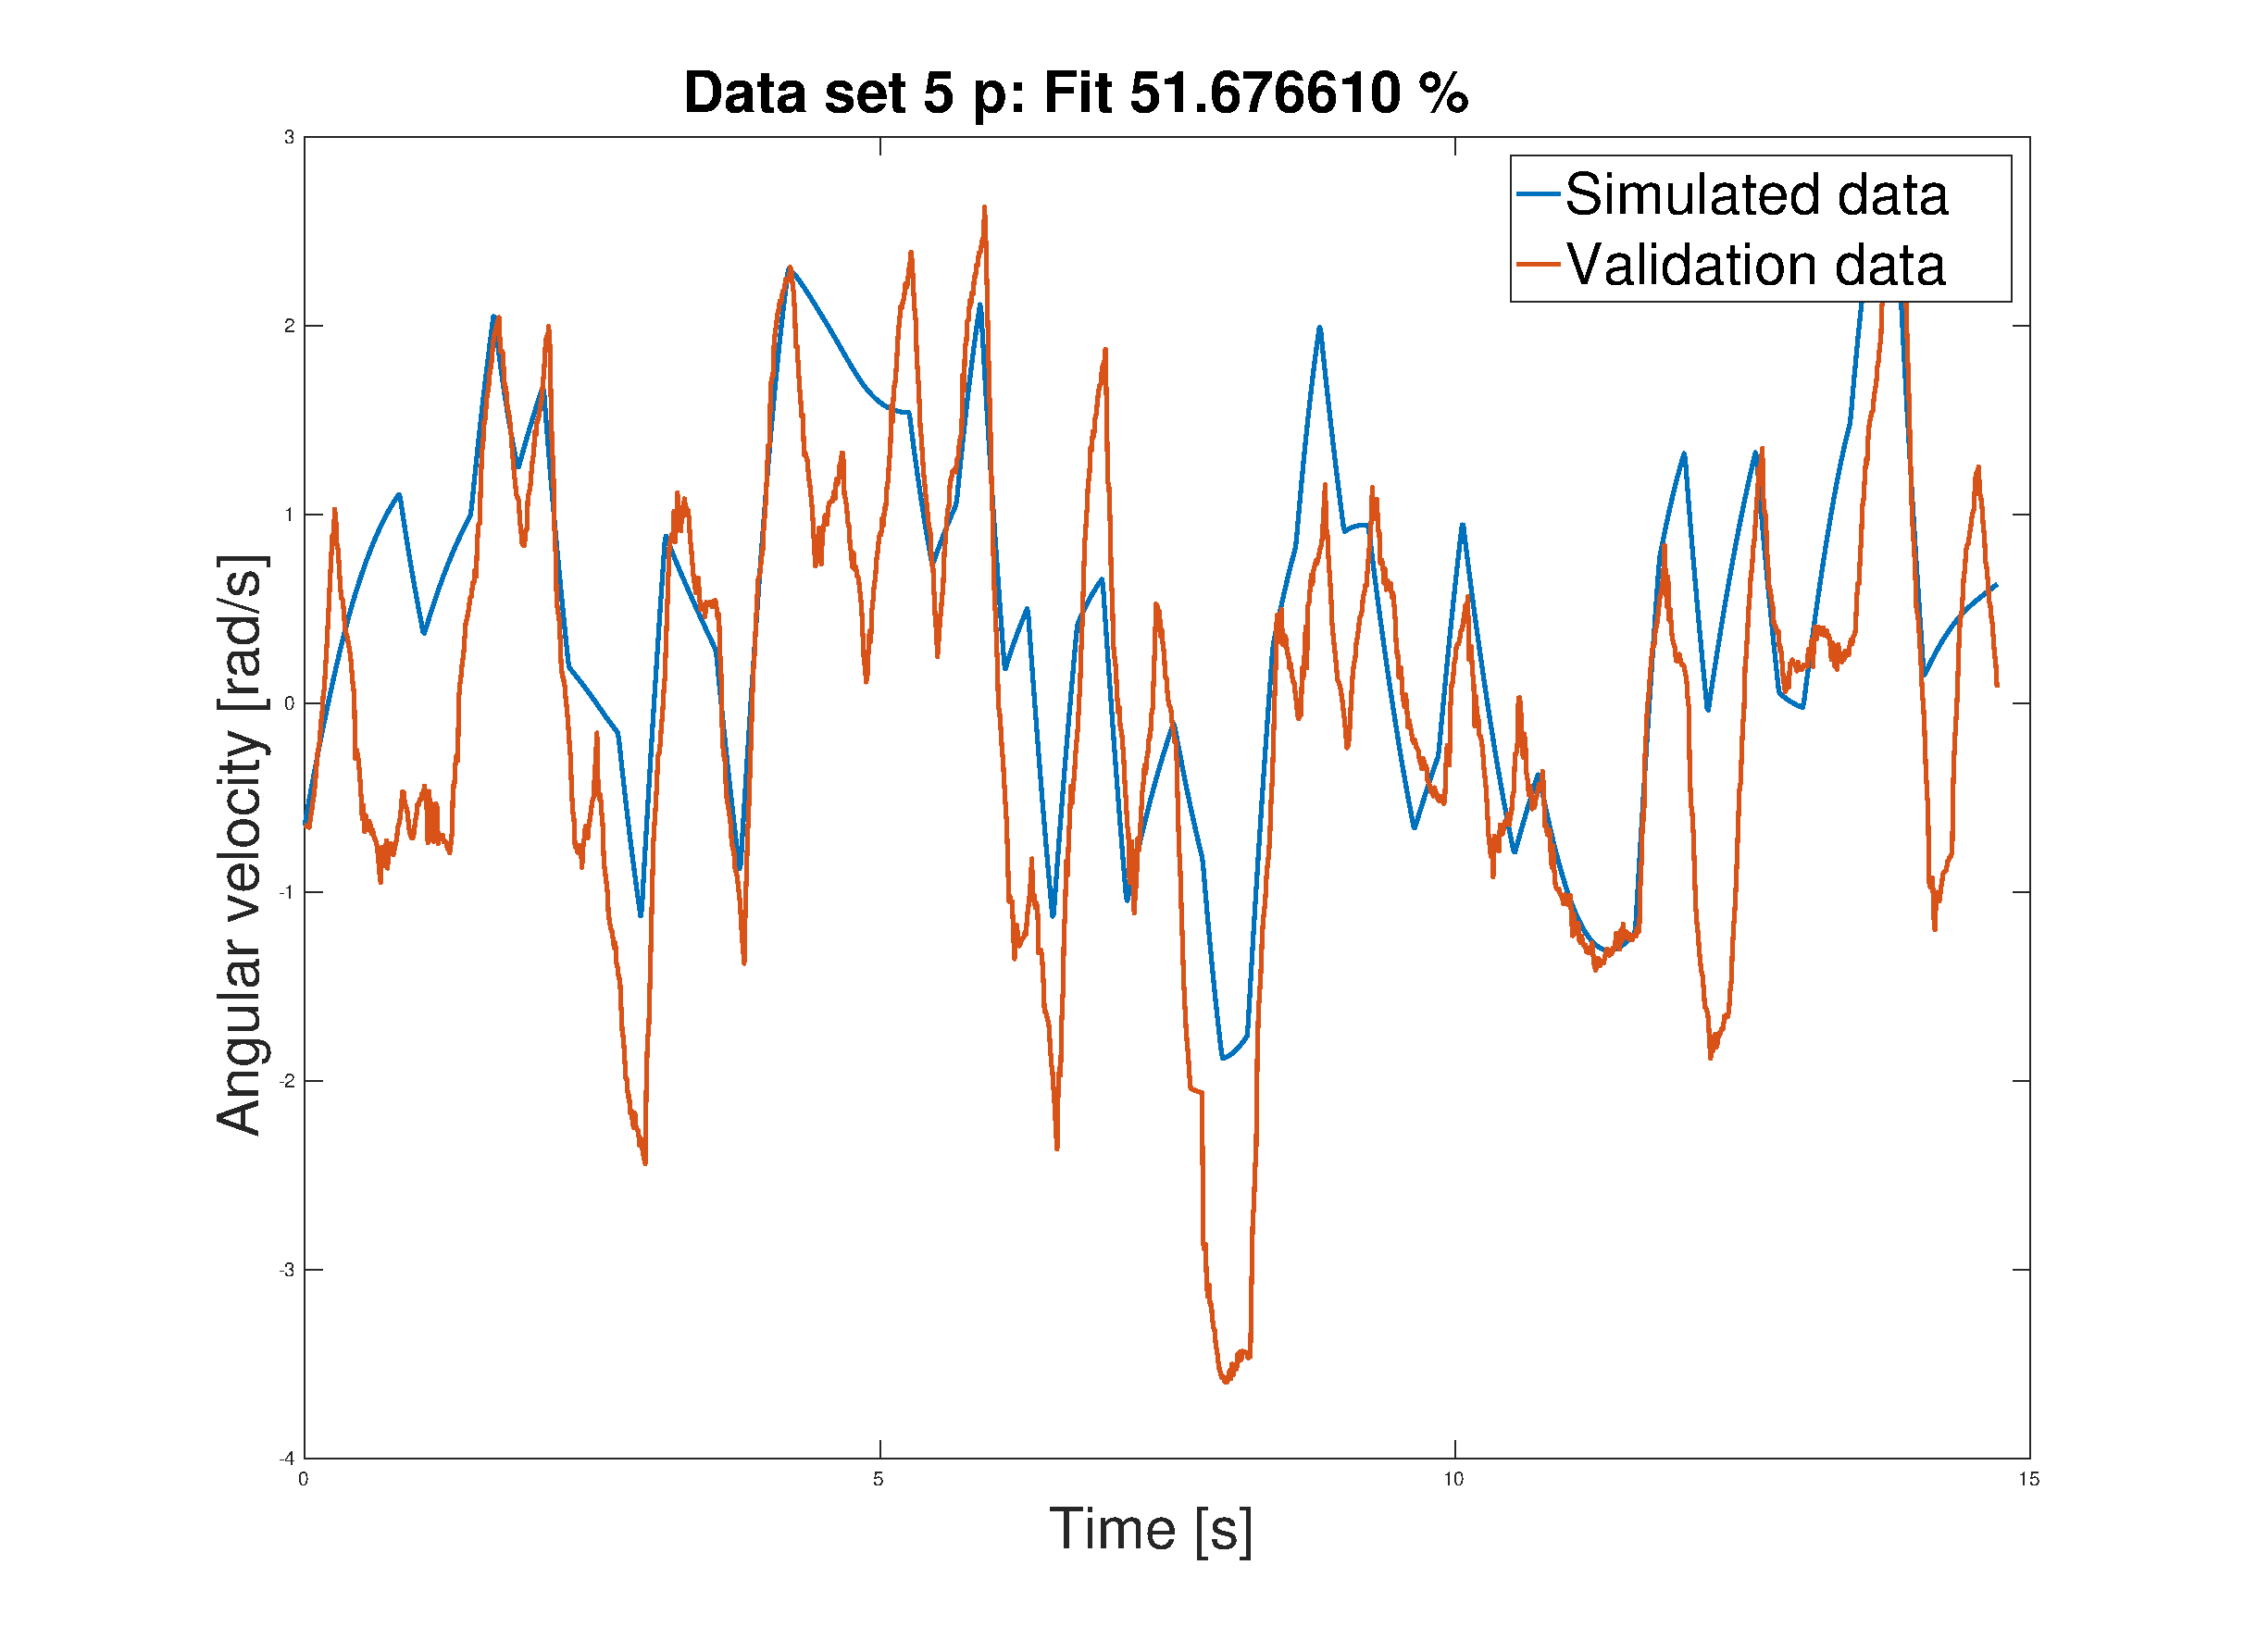
\includegraphics[width=0.5\textwidth]{kalmanEstimatorP}}
  \qquad
  \subfloat[][\label{fig:KalmanCompareQ}Comparison between a simulated model response and validation data in $q$.]{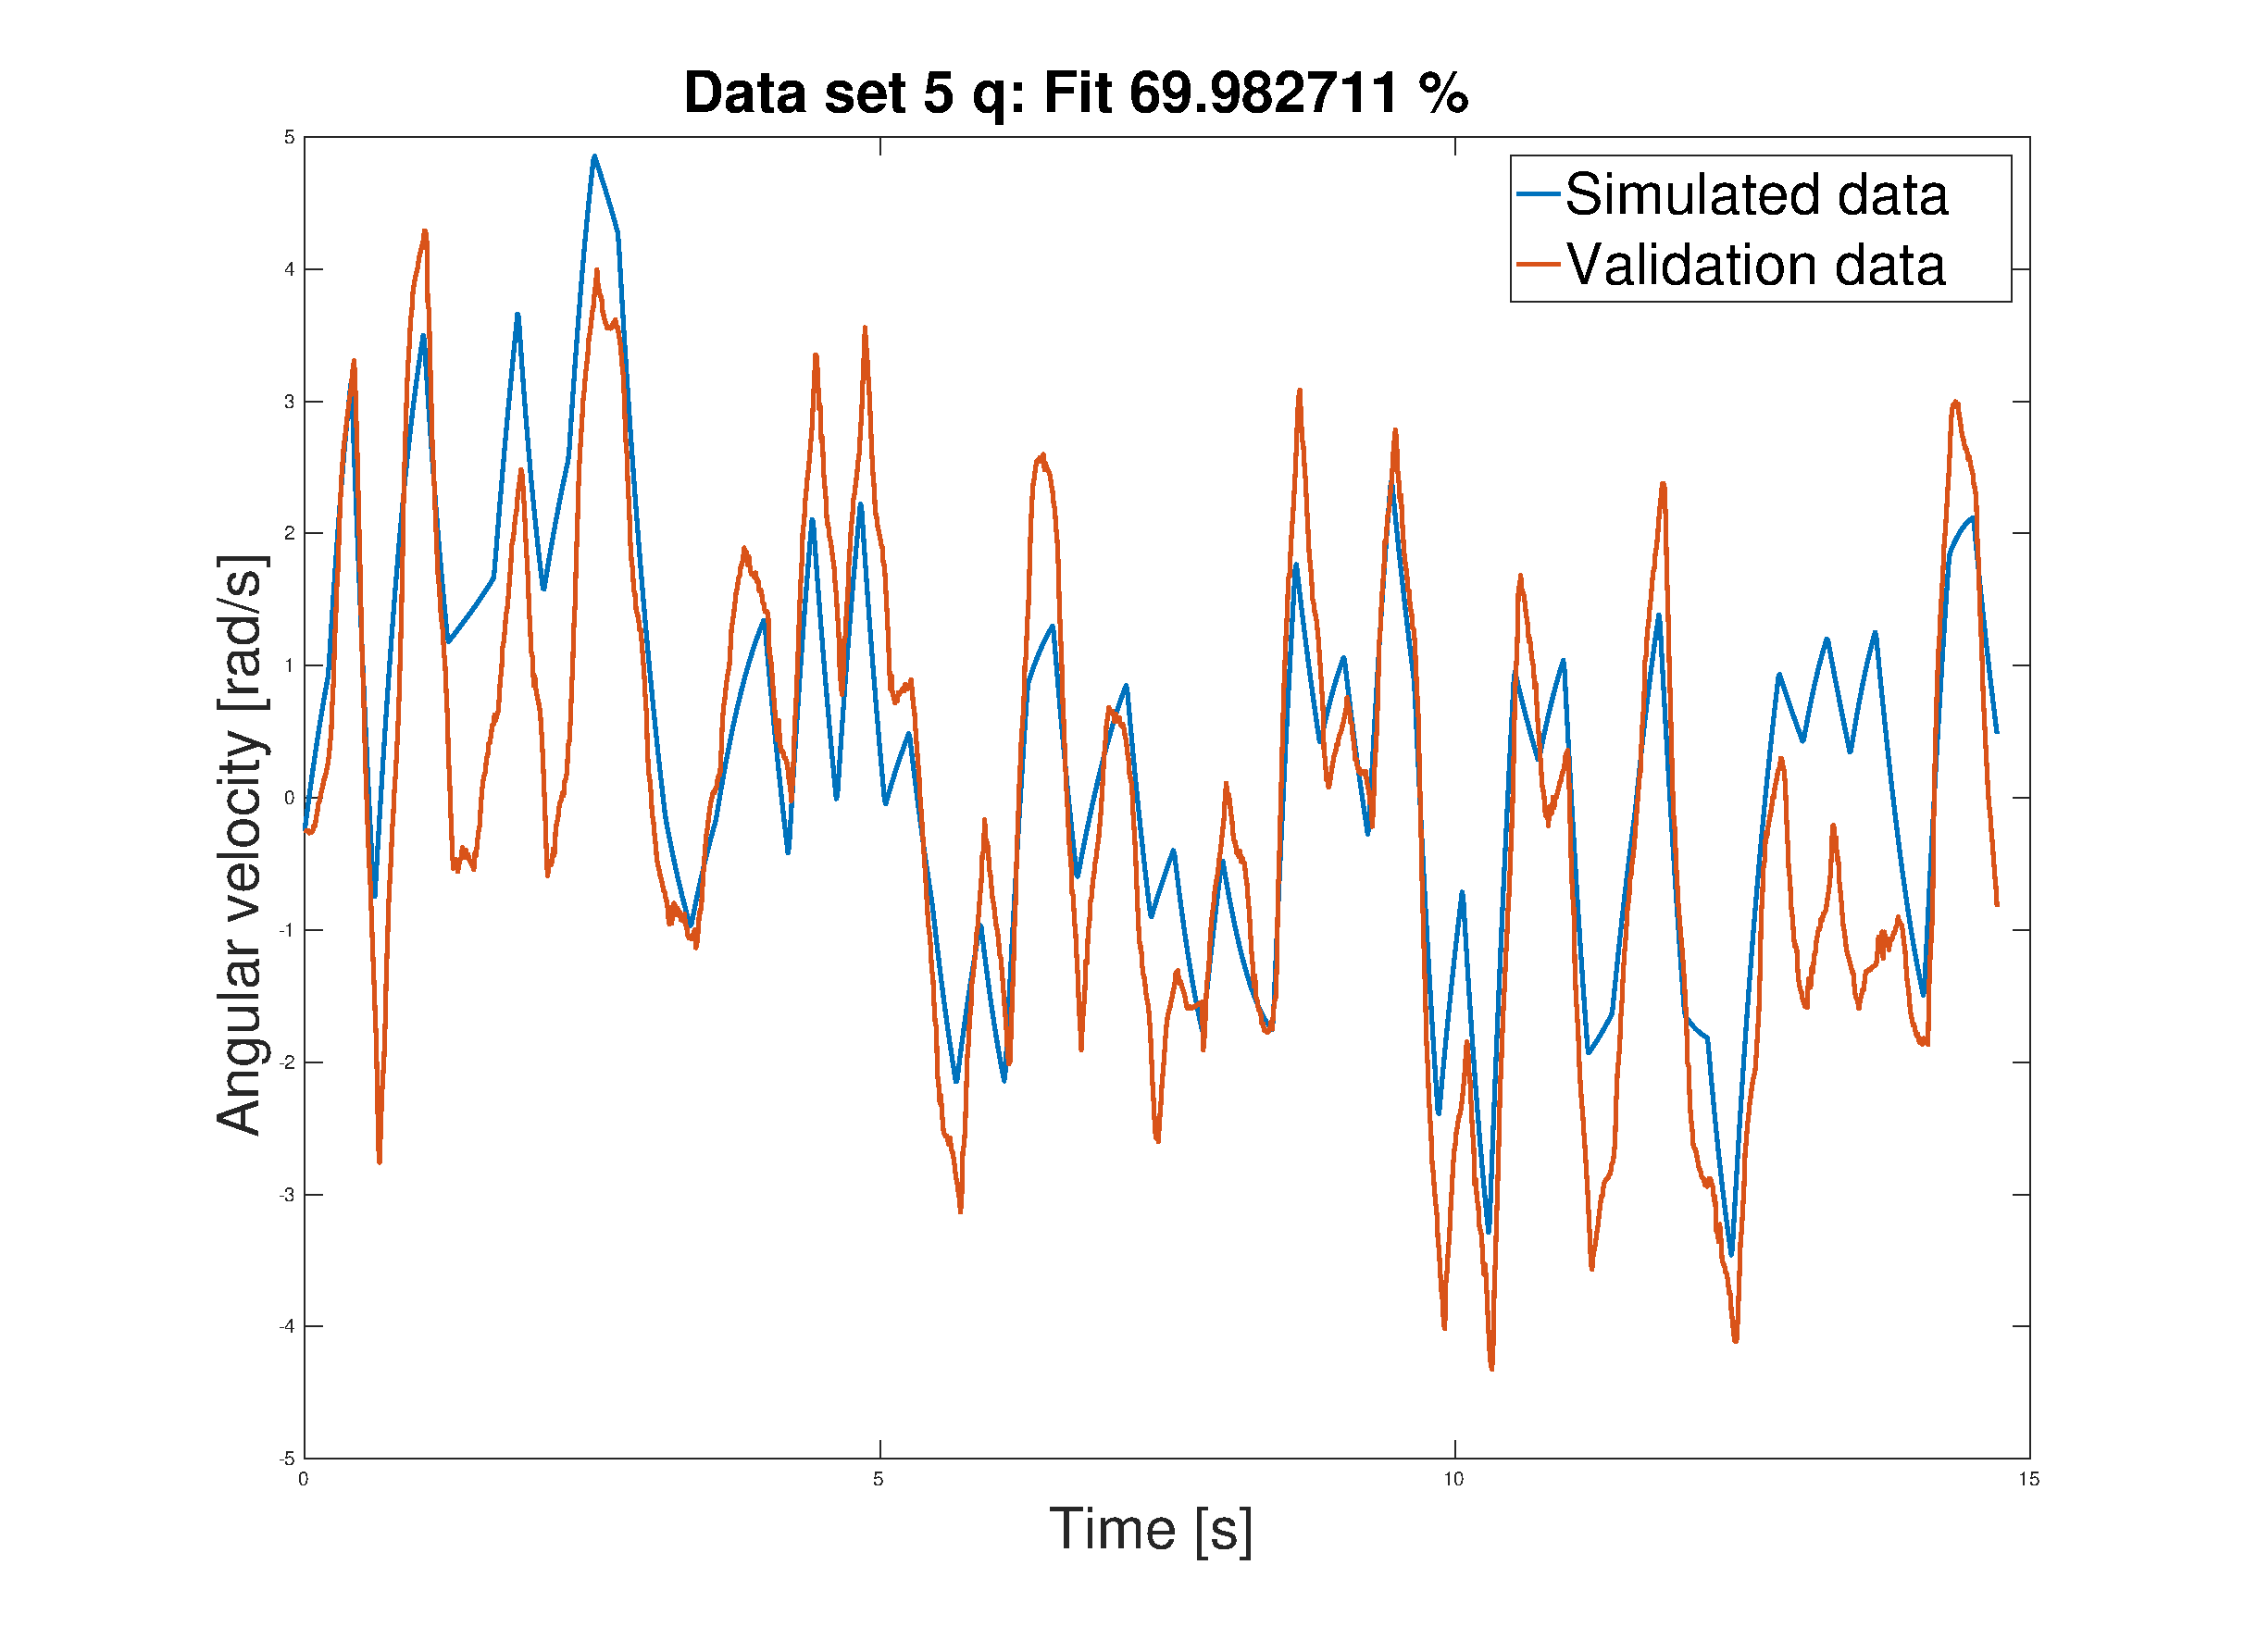
\includegraphics[width=0.5\textwidth]{kalmanEstimatorQ}}
  \\
  \subfloat[][\label{fig:KalmanCompareR}Comparison between a simulated model response and validation data in $r$.]{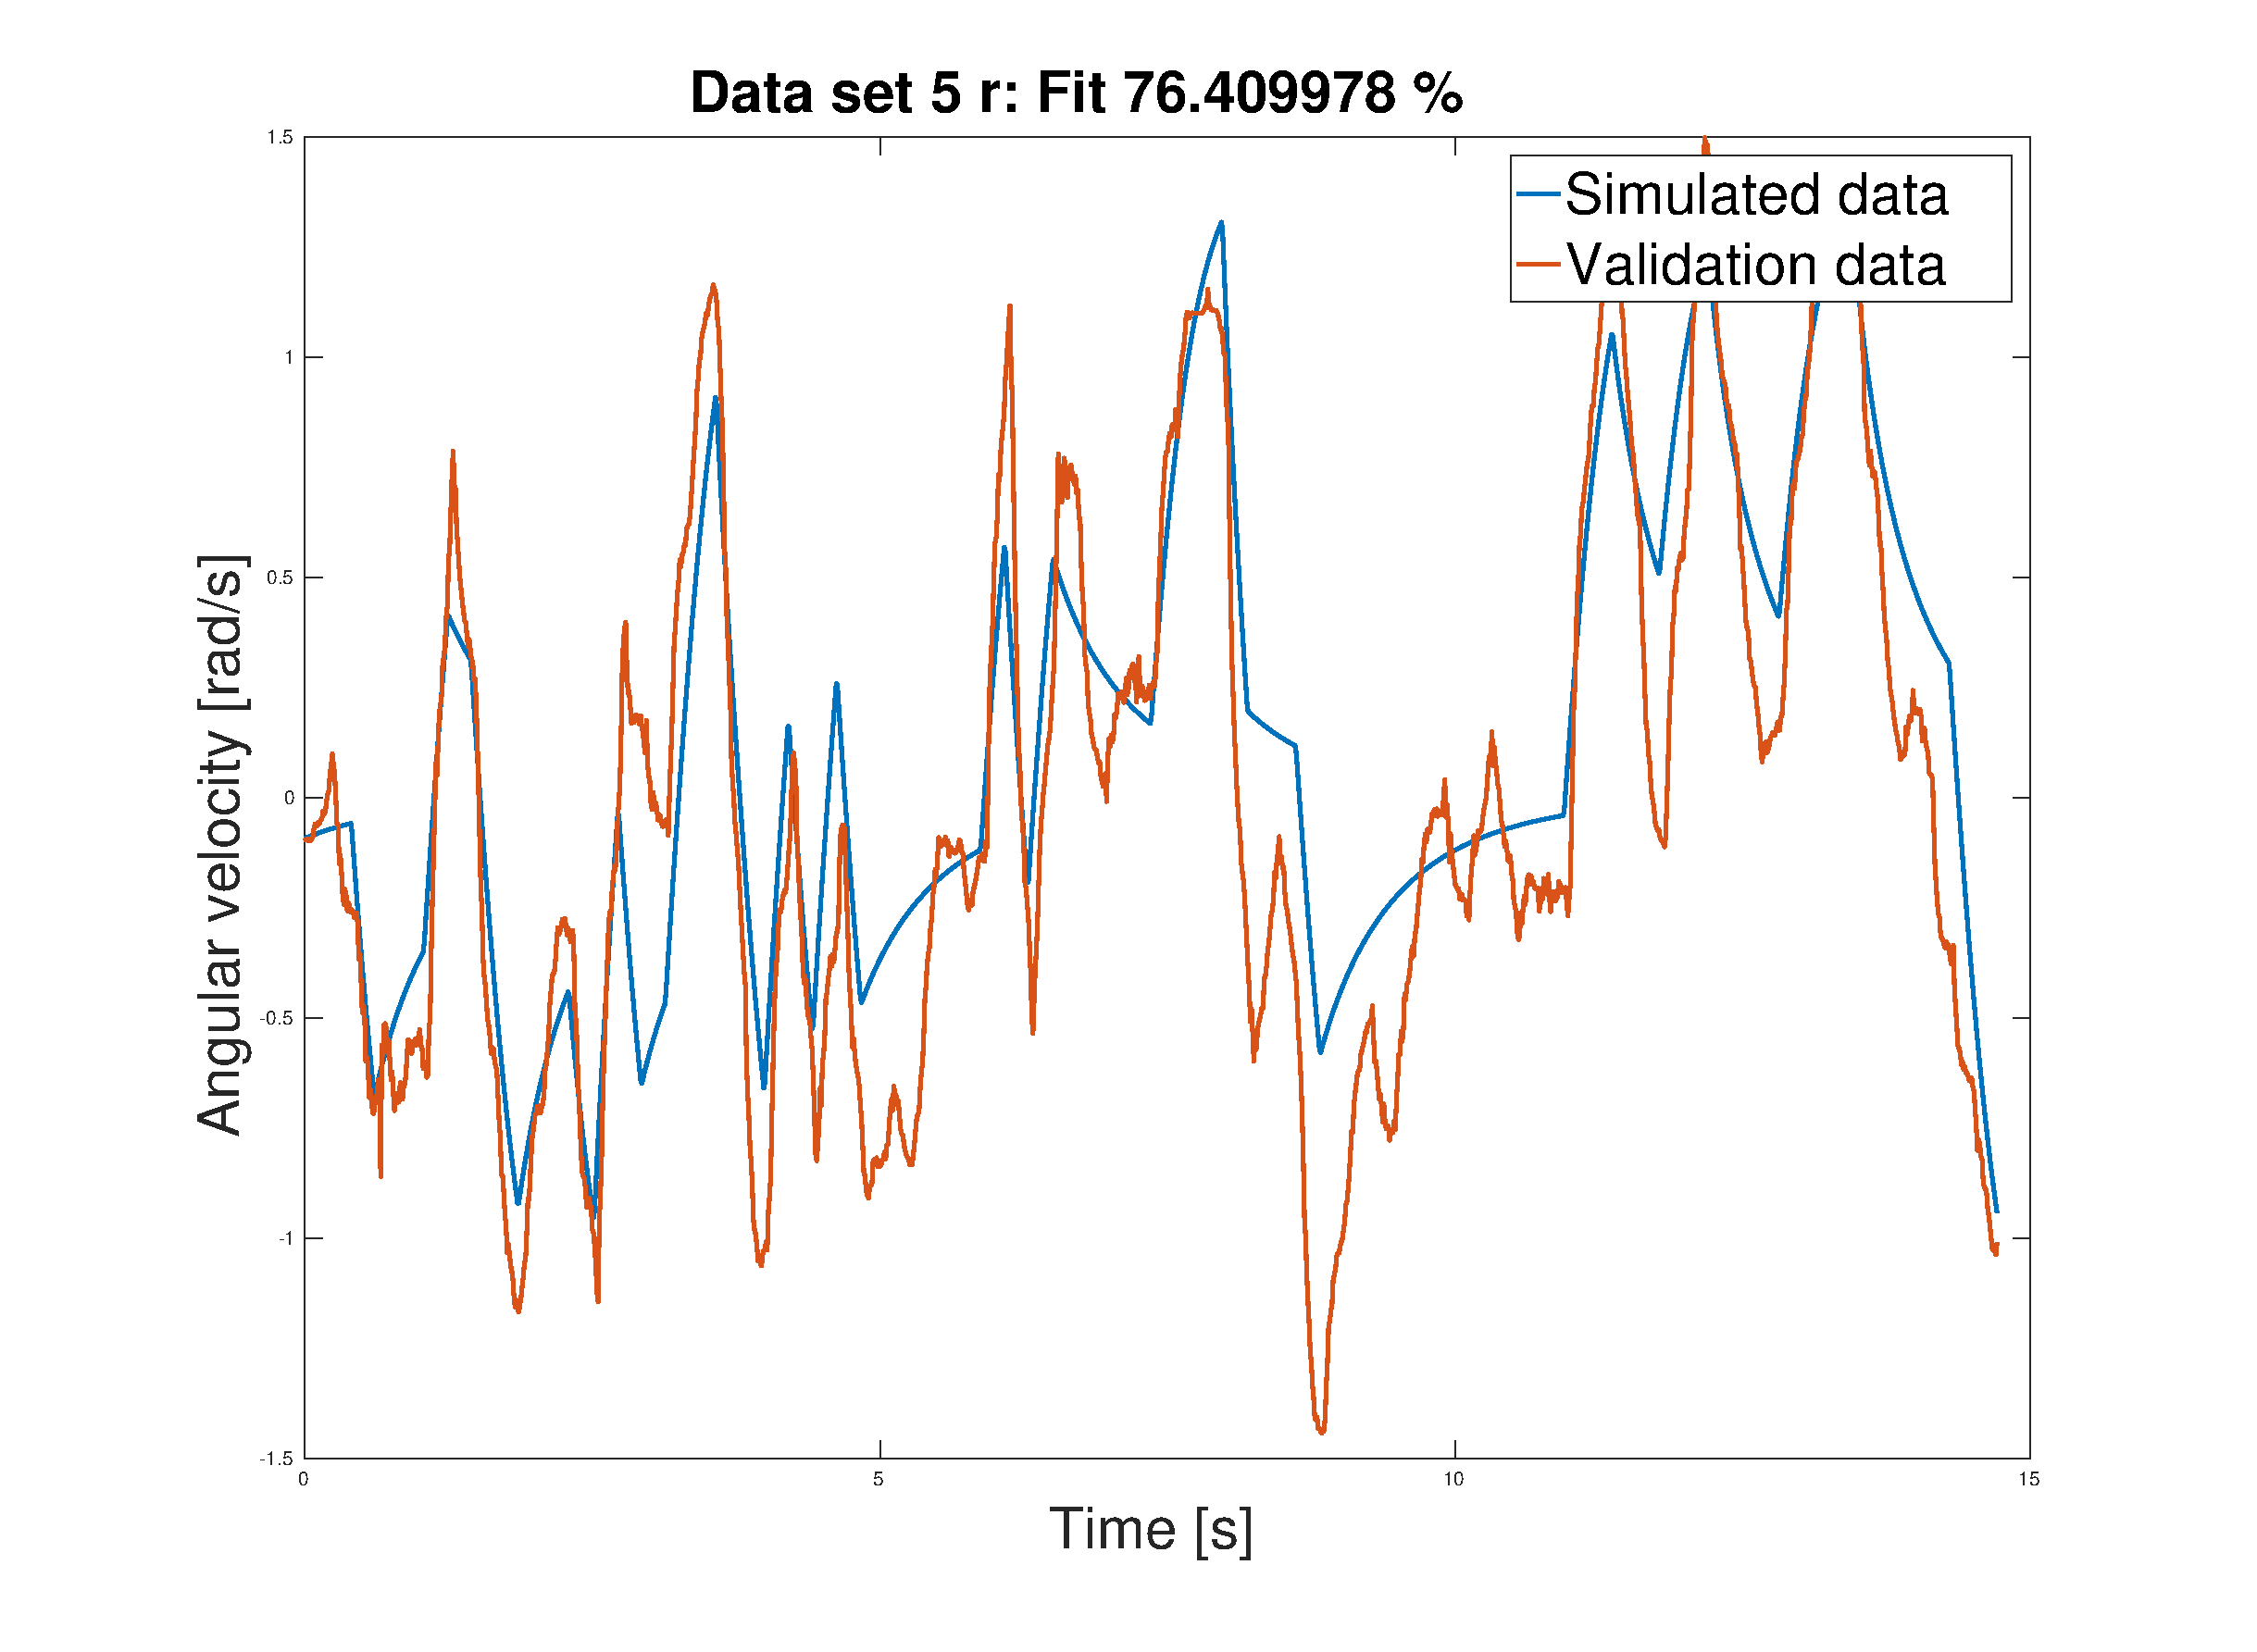
\includegraphics[width=0.5\textwidth]{kalmanEstimatorR}}
  \caption{\label{fig:KalmanCompare}%
    Comparison between simulation of $\nuVector$ (blue) with validation data (red). Goodness of fit statistic can be viewed at the top of each sub-figure.}
\end{figure}





%%%%%%%%%%%%%%%%%%%%%%%%%%%%%%%%%%%%%%%%%%%%%%%%%%%%%%%%%%%
\section{Estimated parameters}
\Tableref{tab:parameterConstants} shows the know and measured parameters used in the \abbrROV. The estimated parameters used in the \abbrROV model are shown in \Tableref{tab:parameterEstimation}.

\begin{table}[tbp]
  \centering
  \caption{\label{tab:parameterConstants}%
    The known parameters used in the \abbrROV model.}
  \begin{tabular}{l l p{0.7\linewidth}}
    \toprule%
    \textbf{Notation}   & \textbf{Value} & \textbf{Description} \\
    \otoprule%
    $m$                 & 6.621 \kilogram                    & Mass of the \abbrROV. \\            
    $g$                 & 9.82  \meter\per\second\squared    & Gravity acceleration.\\   
    $\rho$              & 1000  \kilogram\per\meter\cubed    & Density of water.\\       
    
    $\distance{x}{1}$   & 0.16 \meter & Distance from \abbrCG to thruster 1 in $\xPosition$-direction.\\
    $\distance{y}{1}$   & 0.11 \meter & Distance from \abbrCG to thruster 1 in $\yPosition$-direction.\\
    $\distance{y}{2}$   & 0.11 \meter & Distance from \abbrCG to thruster 2 in $\yPosition$-direction.\\
    $\distance{x}{2}$   & 0.16 \meter & Distance from \abbrCG to thruster 2 in $\xPosition$-direction.\\
    $\distance{y}{3}$   & 0.11 \meter & Distance from \abbrCG to thruster 3 in $\yPosition$-direction.\\
    $\distance{x}{5}$   & 0.20 \meter & Distance from \abbrCG to thruster 5 in $\xPosition$-direction.\\
    $\distance{y}{4}$   & 0.11 \meter & Distance from \abbrCG to thruster 4 in $\yPosition$-direction.\\
    $\distance{z}{6}$   & 0.11 \meter & Distance from \abbrCG to thruster 6 in $\zPosition$-direction.\\
    \bottomrule%
  \end{tabular}
\end{table}


\begin{table}[tbp]
  \centering
  \caption{\label{tab:parameterEstimation}%
    The estimated parameters used in the \abbrROV model.}
  \begin{tabular}{l l p{0.7\linewidth}}
    \toprule%
    \textbf{Notation}   & \textbf{Value} & \textbf{Description} \\
    \otoprule%   
    % Parameters that will be estimated
	$z_B$               & -0.0308 \meter                                      & Distance from \abbrCG to \abbrCB.\\
    $\Kp$               & -1.1082 \kilogram\usk\meter\squared                 & Linear damping coefficient due to rotation in water about the $\xPosition$-axis.\\
    $\Kpabsp$           & -0.3450 \kilogram\usk\meter\squared                 & Quadratic damping coefficient due to rotation in water about the $\xPosition$-axis.\\
    $\Mq$               & -1.2385 \kilogram\usk\meter\squared                 & Linear damping coefficient due to rotation in water about the $\yPosition$-axis.\\
    $\Mqabsq$           & -0.1111 \kilogram\usk\meter\squared                 & Quadratic damping coefficient due to rotation in water about the $\yPosition$-axis.\\
    $\Nr$               & -1.5325 \kilogram\usk\meter\squared                 & Linear damping coefficient due to rotation in water about the $\zPosition$-axis.\\
    $\Nrabsr$           & -1.3977 \kilogram\usk\meter\squared                 & Quadratic damping coefficient due to rotation in water about the $\zPosition$-axis.\\
    $A_p$               & 0.9625  \kilogram\usk\meter\squared                 & Inertia around the $\xPosition$-axis and increased inertia around the $\xPosition$-axis.\\
    $B_q$               & 0.7108  \kilogram\usk\meter\squared                 & Inertia around the $\yPosition$-axis and increased inertia around the $\yPosition$-axis.\\
    $C_r$               & 1.2649  \kilogram\usk\meter\squared                 & Inertia around the $\zPosition$-axis and increased inertia around the $\zPosition$-axis.\\
    \bottomrule%
  \end{tabular}
\end{table}
